% %%%%%%%%%%%%%%%%%%%%%%%%%%%%%%%%%%%%%%%%%%%%%%%%%%%%%%%%%%%%%%%%%%%%%%% %
%                                                                         %
% The Project Gutenberg EBook of A Primer of Quaternions, by Arthur S. Hathaway
%                                                                         %
% This eBook is for the use of anyone anywhere in the United States and most
% other parts of the world at no cost and with almost no restrictions     %
% whatsoever.  You may copy it, give it away or re-use it under the terms of
% the Project Gutenberg License included with this eBook or online at     %
% www.gutenberg.org.  If you are not located in the United States, you'll have
% to check the laws of the country where you are located before using this ebook.
%                                                                         %
%                                                                         %
%                                                                         %
% Title: A Primer of Quaternions                                          %
%                                                                         %
% Author: Arthur S. Hathaway                                              %
%                                                                         %
% Release Date: April 25, 2015 [EBook #9934]                              %
%                                                                         %
% Language: English                                                       %
%                                                                         %
% Character set encoding: ASCII                                           %
%                                                                         %
% *** START OF THIS PROJECT GUTENBERG EBOOK A PRIMER OF QUATERNIONS ***   %
%                                                                         %
% %%%%%%%%%%%%%%%%%%%%%%%%%%%%%%%%%%%%%%%%%%%%%%%%%%%%%%%%%%%%%%%%%%%%%%% %

\def\ebook{9934}
%%%%%%%%%%%%%%%%%%%%%%%%%%%%%%%%%%%%%%%%%%%%%%%%%%%%%%%%%%%%%%%%%%%%%%
%%                                                                  %%
%% Packages and substitutions:                                      %%
%%                                                                  %%
%% book:  Required.                                                 %%
%%                                                                  %%
%% amsmath:  AMS mathematics enhancements. Required.                %%
%% amssymb:  AMS extra symbols. Required.                           %%
%% amsthm:  AMS theorem environments. Required.                     %%
%% makeidx:  Indexing. Required.                                    %%
%%                                                                  %%
%% alltt:    Fixed-width font environment. Required.                %%
%%                                                                  %%
%% graphicx: Graphics. Required.                                    %%
%%                                                                  %%
%% Producer's Comments:                                             %%
%%                                                                  %%
%%   This ebook was originally produced in 2003; boilerplate for    %%
%%   auto-compiling at Project Gutenberg added April 2015.          %%
%%                                                                  %%
%% PDF pages: 85                                                    %%
%% PDF page size: US Letter (8.5 x 11in)                            %%
%%                                                                  %%
%% Images: 34 png diagrams                                          %%
%%                                                                  %%
%% Summary of log file:                                             %%
%% * Three overfull hboxes (10.75pt too wide).                      %%
%% * Two underfull hboxes.                                          %%
%%                                                                  %%
%% Command block:                                                   %%
%%                                                                  %%
%%     pdflatex x2                                                  %%
%%                                                                  %%
%%                                                                  %%
%% April 2015: pglatex.                                             %%
%%   Compile this project with:                                     %%
%%   pdflatex 9934-t.tex ..... TWO times                            %%
%%                                                                  %%
%%   pdfTeX, Version 3.1415926-2.5-1.40.14 (TeX Live 2013/Debian)   %%
%%                                                                  %%
%%%%%%%%%%%%%%%%%%%%%%%%%%%%%%%%%%%%%%%%%%%%%%%%%%%%%%%%%%%%%%%%%%%%%%
\listfiles
\documentclass[oneside,12pt]{book}[2005/09/16]

%%%%%%%%%%%%%%%%%%%%%%%%%%%%% PACKAGES %%%%%%%%%%%%%%%%%%%%%%%%%%%%%%%
\usepackage[leqno]{amsmath}[2000/07/18] %% Displayed equations
\usepackage{amssymb}[2009/06/22]
\usepackage{amsthm}[2009/07/02]

\usepackage{alltt}[1997/06/16]   %% boilerplate, credits, license

\usepackage{graphicx}[1999/02/16]

\providecommand{\ebook}{00000}    % Overridden during white-washing

%%%% Fixed-width environment to format PG boilerplate %%%%
\newenvironment{PGtext}{%
\begin{alltt}
\fontsize{9.2}{10.5}\ttfamily\selectfont}%
{\end{alltt}}

%%%% Global style parameters %%%%
% Loosen horizontal spacing
\allowdisplaybreaks[1]
\setlength{\emergencystretch}{1.5em}
\newcommand{\loosen}{\spaceskip 0.5em plus 1em minus 0.25em}

%%%% Major document divisions %%%%
\newcommand{\PGBoilerPlate}{%
  \frontmatter
  \pagenumbering{Alph}
  \pagestyle{empty}
}
\newcommand{\PGLicense}{%
  \backmatter
  \pagenumbering{Roman}
}

\newcommand{\TranscribersNote}{%
  \begin{minipage}{0.85\textwidth}
    \small
    \subsection*{\centering\normalfont\scshape\normalsize Transcriber's Note}
      Minor typographical corrections and presentational changes have been
  made without comment. The \LaTeX\ source file may be downloaded from
  \begin{center}
    \texttt{www.gutenberg.org/ebooks/\ebook}.
  \end{center}
  \end{minipage}
}

\newcommand{\MainMatter}
{
  \mainmatter
  \pagenumbering{arabic}
  \pagestyle{plain}
}

%%%%%%%%%%%%%%%%%%%%%%%% START OF DOCUMENT %%%%%%%%%%%%%%%%%%%%%%%%%%
\begin{document}
%%%% PG BOILERPLATE %%%%
\PGBoilerPlate
\begin{center}
\begin{minipage}{\textwidth}
\small
\begin{PGtext}
The Project Gutenberg EBook of A Primer of Quaternions, by Arthur S. Hathaway

This eBook is for the use of anyone anywhere in the United States and most
other parts of the world at no cost and with almost no restrictions
whatsoever.  You may copy it, give it away or re-use it under the terms of
the Project Gutenberg License included with this eBook or online at
www.gutenberg.org.  If you are not located in the United States, you'll have
to check the laws of the country where you are located before using this ebook.



Title: A Primer of Quaternions

Author: Arthur S. Hathaway

Release Date: April 25, 2015 [EBook #9934]

Language: English

Character set encoding: ASCII

*** START OF THIS PROJECT GUTENBERG EBOOK A PRIMER OF QUATERNIONS ***
\end{PGtext}
\end{minipage}
\end{center}
\clearpage

%%%% Credits and transcriber's note %%%%
\begin{center}
\begin{minipage}{\textwidth}
\begin{PGtext}
Produced by Cornell University, Joshua Hutchinson, John
Hagerson, and the Online Distributed Proofreading Team
\end{PGtext}
\end{minipage}
\vfill
\TranscribersNote
\end{center}
%%%%%%%%%%%%%%%%%%%%%%%%%%% FRONT MATTER %%%%%%%%%%%%%%%%%%%%%%%%%%
\cleardoublepage

\iffalse %%%%% Start of original header %%%%
\documentclass[oneside]{book}
\usepackage[leqno]{amsmath}
\usepackage{amssymb,amsthm,graphicx}
\begin{document}
\frontmatter

\thispagestyle{empty}
\small
\begin{verbatim}

\end{verbatim}
\normalsize
\fi
%%%%% End of original header %%%%
\newpage

\begin{center}
\bigskip \huge
A PRIMER OF QUATERNIONS

\bigskip\bigskip
\footnotesize BY

\bigskip
\large ARTHUR S. HATHAWAY

\bigskip
\footnotesize PROFESSOR OF MATHEMATICS IN THE ROSE POLYTECHNIC \\
INSTITUTE, TERRE HAUTE, IND.

\bigskip\bigskip
\normalsize 1896
\end{center}

\newpage

\pagenumbering{roman}
\pagestyle{plain}

\section*{Preface}

The Theory of Quaternions is due to Sir William Rowan Hamilton,
Royal Astronomer of Ireland, who presented his first paper on the
subject to the Royal Irish Academy in 1843. His Lectures on
Quaternions were published in 1853, and his Elements, in 1866,
shortly after his death. The Elements of Quaternions by Tait is
the accepted text-book for advanced students.

The following development of the theory is prepared for average
students with a thorough knowledge of the elements of algebra and
geometry, and is believed to be a simple and elementary treatment
founded directly upon the fundamental ideas of the subject. This
theory is applied in the more advanced examples to develop the
principal formulas of trigonometry and solid analytical geometry,
and the general properties and classification of surfaces of
second order.

In the endeavour to bring out the \textit{number} idea of
Quaternions, and at the same time retain the established
nomenclature of the analysis, I have found it necessary to abandon
the term ``\textit{vector}'' for a directed length. I adopt
instead Clifford's suggestive name of ``\textit{step},'' leaving
to ``\textit{vector}'' the sole meaning of ``\textit{right
quaternion}.'' This brings out clearly the relations of this
number and line, and emphasizes the fact that Quaternions is a
natural extension of our fundamental ideas of number, that is
subject to ordinary principles of geometric representation, rather
than an artificial species of geometrical algebra.

The physical conceptions and the breadth of idea that the subject
of Quaternions will develop are, of themselves, sufficient reward
for its study. At the same time, the power, directness, and
simplicity of its analysis cannot fail to prove useful in all
physical and geometrical investigations, to those who have
thoroughly grasped its principles.

On account of the universal use of analytical geometry, many
examples have been given to show that Quaternions in its
semi-cartesian form is a direct development of that subject. In
fact, the present work is the outcome of lectures that I have
given to my classes for a number of years past as the equivalent
of the usual instruction in the analytical geometry of space. The
main features of this primer were therefore developed in the
laboratory of the class-room, and I desire to express my thanks to
the members of my classes, wherever they may be, for the interest
that they have shown, and the readiness with which they have
expressed their difficulties, as it has been a constant source of
encouragement and assistance in my work.

I am also otherwise indebted to two of my students,---to Mr.\
H.~B.\ Stilz for the accurate construction of the diagrams, and to
Mr.\ G.\ Willius for the plan (upon the cover) of the plagiograph
or mechanical quaternion multiplier which was made by him while
taking this subject. The theory of this instrument is contained in
the step proportions that are given with the diagram.\footnote{See
Example 19, Chapter I.}

\begin{flushright}
ARTHUR S.\ HATHAWAY.
\end{flushright}

\tableofcontents

\MainMatter
\chapter{Steps}

\addcontentsline{toc}{section}{Definitions and Theorems}

\begin{enumerate}

\item \textsc{Definition.} \textit{A step is a given length
measured in a given direction.}

\textit{E.g., 3 feet east, 3 feet north, 3 feet up, 3 feet
north-east, 3 feet north-east-up,} are steps.

\item \textsc{Definition.} \textit{Two steps are equal when, and
only when, they have the same lengths and the same directions.}

\textit{E.g., 3 feet east}, and \textit{3 feet north}, are not
equal steps, because they differ in direction, although their
lengths are the same; and \textit{3 feet east, 5 feet east}, are
not equal steps, because their lengths differ, although their
directions are the same; but all steps of \textit{3 feet east} are
equal steps, whatever the points of departure.

\item We shall use bold-faced $\mathbf{AB}$ to denote the step
whose length is $AB$, and whose direction is from $A$ towards $B$.

\begin{center}
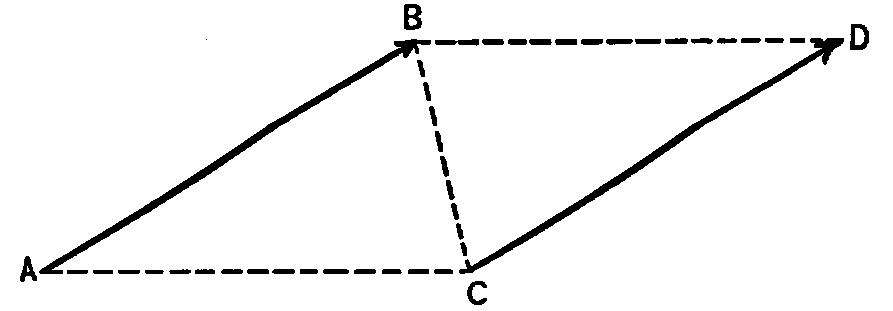
\includegraphics[width=80mm]{images/Image1.png}
\end{center}

Two steps $\mathbf{AB}$, $\mathbf{CD}$, are obviously equal when,
and only when, $ABDC$ is a parallelogram.

\item \textsc{Definition.} \textit{If several steps be taken in
succession, so that each step begins where the preceding step
ends, the step from the beginning of the first to the end of the
last step is the sum of those steps.}

\begin{center}
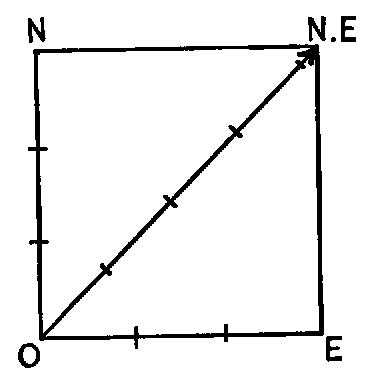
\includegraphics[width=80mm]{images/Image2.png}
\end{center}

\textit{E.g., 3 feet east + 3 feet north = $3\sqrt{2}$ feet
north-east = 3 feet north + 3 feet east}. Also $\mathbf{AB + BC =
AC}$, whatever points $A$, $B$, $C$, may be. Observe that this
equality between \textit{steps} is not a length equality, and
therefore does not contradict the inequality $AB + BC > AC$, just
as 5 \textit{dollars credit} + 2 \textit{dollars debit} = 3
\textit{dollars credit} does not contradict the inequality
\textit{5 dollars + 2 dollars $>$ 3 dollars}.

\begin{center}
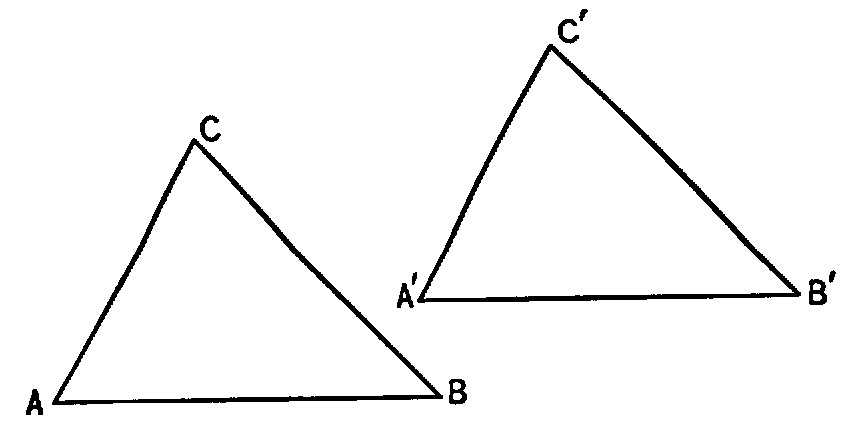
\includegraphics[width=80mm]{images/Image3.png}
\end{center}

\item \textit{If equal steps be added to equal steps, the sums are
equal steps.}

Thus if $\mathbf{AB = A'B'}$, and $\mathbf{BC=B'C'}$, then
$\mathbf{AC = A'C'}$, since the triangles $ABC$, $A'B'C'$ must be
equal triangles with the corresponding sides in the same
direction.

\item \textit{A sum of steps is commutative} (\textit{i.e.}, the
components of the sum may be added in any order without changing
the value of the sum).

\begin{center}
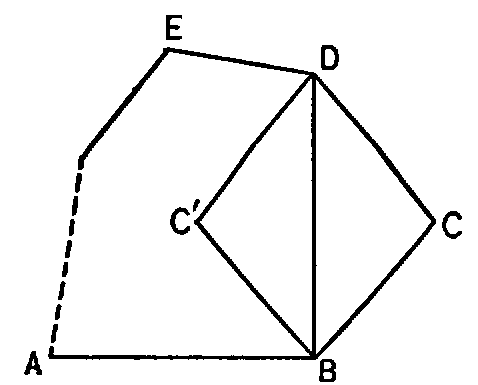
\includegraphics[width=80mm]{images/Image4.png}
\end{center}

For, in the sum $\mathbf{AB + BC + CD + DE + \cdots}$, let
$\mathbf{BC' = CD}$; then since $BCDC'$ is a parallelogram,
therefore $\mathbf{C'D = BC}$, and the sum with $\mathbf{BC}$,
$\mathbf{CD}$, interchanged is $\mathbf{AB + BC' + C'D + DE +
\cdots}$, which has the same value as before. By such
interchanges, the sum can be brought to any order of adding.

\item \textit{A sum of steps is associative} (\textit{i.e}., any
number of consecutive terms of the sum may be replaced by their
sum without changing the value of the whole sum).

For, in the sum $\mathbf{AB + BC + CD + DE + \cdots}$, let
$\mathbf{BC}$, $\mathbf{CD}$, be replaced by their sum
$\mathbf{BD}$; then the new sum is $\mathbf{AB + BD + DE +
\cdots}$, whose value is the same as before; and similarly for
other consecutive terms.

\item \textit{The product of a step by a positive number is that
step lengthened by the multiplier without change of direction.}

\textit{E.g.}, $\mathbf{2AB = AB + AB}$, which is $\mathbf{AB}$
doubled in length without change of direction; similarly $\frac
{1}{2}\mathbf{AB} = $(step that doubled gives $\mathbf{AB}$) $=$
($\mathbf{AB}$ halved in length without change of direction). In
general, $m\mathbf{AB} = m$ lengths $AB$ measured in the direction
$\mathbf{AB}$; $\frac{1}{n} \mathbf{AB} = \frac {1}{n}$th of
length $AB$ measured in the direction $\mathbf{AB}$; etc.

\item \textit{The negative of a step is that step reversed in
direction without change of length}.

For the negative of a quantity is that quantity which added to it
gives zero; and since $\mathbf{AB + BA = AA} = 0$, therefore
$\mathbf{BA}$ is the negative of $\mathbf{AB}$, or
$\mathbf{BA=-AB}$.

\begin{itemize}
\item \textsc{Cor.\ 1.} \textit{The product of a step by a negative
number is that step lengthened by the number and reversed in
direction.}

For $-n\mathbf{AB}$ is the negative of $n\mathbf{AB}$.

\item \textsc{Cor.\ 2.} \textit{A step is subtracted by reversing
its direction and adding it.}

For the result of subtracting is the result of adding the negative
quantity. \textit{E.g.}, $\mathbf{AB-CB = AB+BC = AC}$.
\end{itemize}

\item \textit{A sum of steps is multiplied by a given number by
multiplying the components of the sum by the number and adding the
products.}

\begin{center}
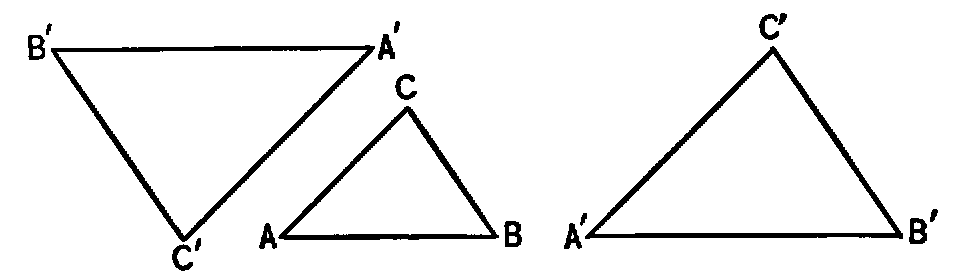
\includegraphics[width=80mm]{images/Image5.png}
\end{center}

Let $n \cdot \mathbf{AB = A'B'}, n \cdot \mathbf{BC=BC'}$; then
$ABC, A'B'C'$ are similar triangles, since the sides about $B$,
$B'$ are proportional, and in the same or opposite directions,
according as $n$ is positive or negative; therefore $AC$, $A'C'$
are in the same or opposite directions and in the same ratio;
\textit{i.e.}, $n\mathbf{AC = A'C'}$, which is the same as
$n(\mathbf{AB+BC}) = n\mathbf{AB}+n\mathbf{BC}$.

This result may also be stated in the form: \textit{a multiplier
is distributive over a sum}.

\item \textit{Any step may be resolved into a multiple of a given
step parallel to it; and into a sum of multiples of two given
steps in the same plane with it that are not parallel; and into a
sum of multiples of three given steps that are not parallel to one
plane.}

\begin{center}
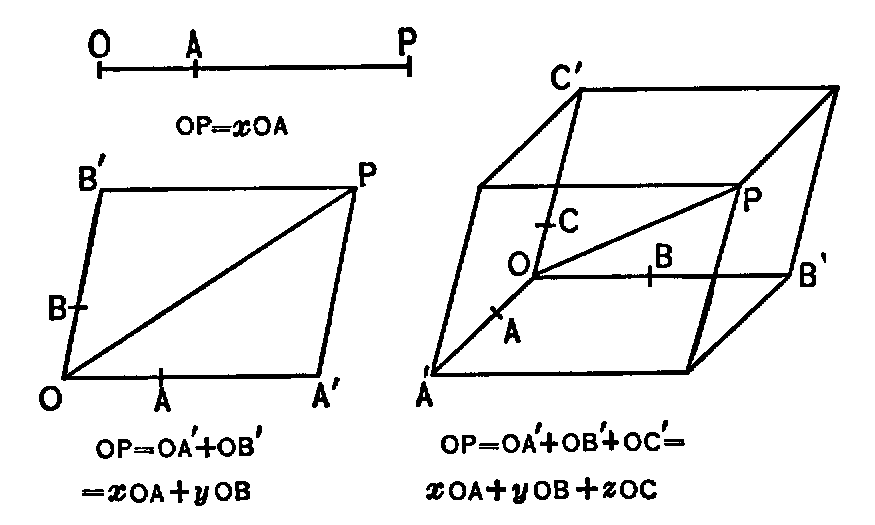
\includegraphics[width=80mm]{images/Image6.png}
\end{center}

\item It is obvious that if the sum of two finite steps is zero,
then the two steps must be parallel; in fact, if one step is
$\mathbf{AB}$, then the other must be equal to $\mathbf{BA}$.
Also, if the sum of three finite steps is zero, then the three
steps must be parallel to one plane; in fact, if the first is
$\mathbf{AB}$, and the second is $\mathbf{BC}$, then the third
must be equal to $\mathbf{CA}$. Hence, \textit{if a sum of steps
on two lines that are not parallel (or on three lines that are not
parallel to one plane) is zero, then the sum of the steps on each
line is zero,} since, as just shown, the sum of the steps on each
line cannot be finite and satisfy the condition that their sum is
zero. We thus see that an equation between steps of one plane can
be separated into two equations by resolving each step parallel to
two intersecting lines of that plane, and that an equation between
steps in space can be separated into three equations by resolving
each step parallel to three lines of space that are not parallel
to one plane. We proceed to give some applications of this and
other principles of step analysis in locating a point or a locus
of points with respect to given data (Arts.\ 13-20).

\addcontentsline{toc}{section}{Centre of Gravity}
\section*{Centre of Gravity}

\item \textit{The point $P$ that satisfies the condition
$l\mathbf{AP} + m\mathbf{BP} = 0$ lies upon the line $AB$ and
divides $AB$ in the inverse ratio of $l:m$ (i.e., $P$ is the
centre of gravity of a mass $l$ at $A$ and a mass $m$ at $B$).}

The equation gives $l\mathbf{AP} = m\mathbf{PB}$; hence:

$\mathbf{AP}$, $\mathbf{PB}$ are parallel; $P$ lies on the line
$AB$; and $\mathbf{AP}:\mathbf{PB} = m:l = $ \textit{inverse of}
$l:m$.

If $l:m$ is positive, then $\mathbf{AP}$, $\mathbf{PB}$ are in the
same direction, so that $P$ must lie between $A$ and $B$; and if
$l:m$ is negative, then $P$ must lie on the line $AB$ produced. If
$l = m$, then $P$ is the middle point of $AB$; if $l=-m$, then
there is no finite point $P$ that satisfies the condition, but $P$
satisfies it more nearly, the farther away it lies upon $AB$
produced, and this fact is expressed by saying that \textit{``$P$
is the point at infinity on the line $AB$.''}

\item By substituting $\mathbf{AO + OP}$ for $\mathbf{AP}$ and
$\mathbf{BO + OP}$ for $\mathbf{BP}$ in $l\mathbf{AP} +
m\mathbf{BP} = 0$, and transposing known steps to the second
member, we find the point $P$ with respect to any given origin
$O$, viz.,

\begin{enumerate}
\item $(l+m)\mathbf{OP} = l\mathbf{OA} + m\mathbf{OB}$, where $P$
divides $AB$ inversely as $l:m$.
\end{enumerate}

\begin{center}
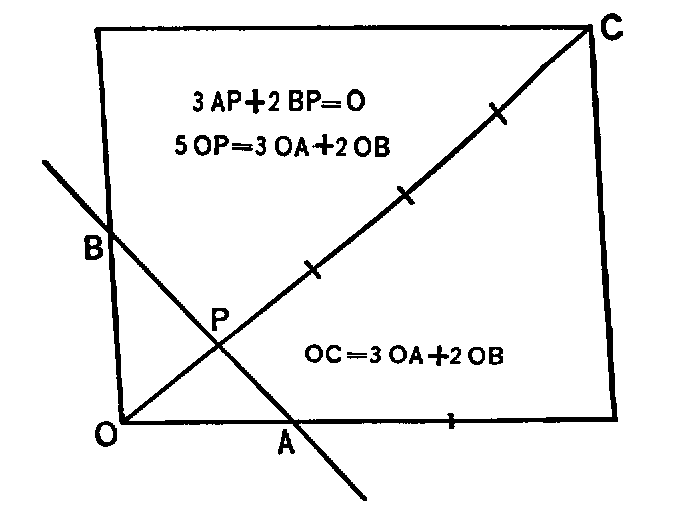
\includegraphics[width=80mm]{images/Image7.png}
\end{center}

\begin{itemize}
\item \textsc{Cor.} \textit{If $\mathbf{OC} = l\mathbf{OA} +
m\mathbf{OB}$, then $OC$, produced if necessary, cuts $AB$ in the
inverse ratio of $l:m$, and $\mathbf{OC}$ is $(l + m)$ times the
step from $O$ to the point of division.}

For, if $P$ divide $AB$ inversely as $l:m$, then by \textit{(a)}
and the given equation, we have
\begin{equation*}
\mathbf{OC}=(l+m)\mathbf{OP}.
\end{equation*}
\end{itemize}

\item \textit{The point $P$ that satisfies the condition
$l\mathbf{AP} + m\mathbf{BP} + n\mathbf{CP} = 0$ lies in the plane
of the triangle $ABC$; $AP$ (produced) cuts $BC$ at a point $D$
that divides $BC$ inversely as $m:n$, and $P$ divides $AD$
inversely as $l:m+n$ (i.e., $P$ is the center of gravity of a mass
$l$ at $A$, a mass $m$ at $B$, and a mass $n$ at $C$). Also the
triangles $PBC$, $PCA$, $PAB$, $ABC$, are proportional to $l$,
$m$, $n$, $l+m+n$.}

\begin{center}
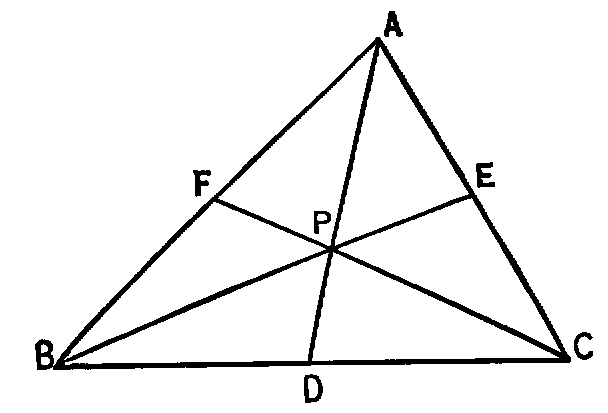
\includegraphics[width=80mm]{images/Image8.png}
\end{center}

The three steps $l\mathbf{AP}$, $m\mathbf{BP}$, $n\mathbf{CP}$
must be parallel to one plane, since their sum is zero, and hence
$P$ must lie in the plane of $ABC$. Since $\mathbf{BP=BD + DP}$,
$\mathbf{CP = CD + DP}$, the equation becomes, by making these
substitutions, $l\mathbf{AP} + (m+n)\mathbf{DP} + m\mathbf{BD} +
n\mathbf{CD} = 0$. This is an equation between steps on the two
intersecting lines, $AD$, $BC$, and hence the resultant step along
each line is zero; i.e., $m\mathbf{BD} + n\mathbf{CD} = 0$ (or $D$
divides $BC$ inversely as $m:n$), and

\begin{equation}
\tag{a} l\mathbf{AP} + (m+n)\mathbf{DP} = 0
\end{equation}

(or $P$ divides $AD$ inversely as $l:m+n$). Also, we have, by
adding $l\mathbf{PD} + l\mathbf{DP} = 0$ to (\textit{a}),
\begin{equation*}
l\mathbf{AD}+(l+m+n)\mathbf{DP} = 0.
\end{equation*}
Hence
\begin{equation*}
l:l+m+n = \mathbf{PD:AD} = PBC:ABC,
\end{equation*}
since the triangles $PBC$, $ABC$ have a common base $BC$, (We must
take the ratio of these triangles as positive or negative
according as the vertices $P$, $A$ lie on the same or opposite
sides of the base $BC$, since the ratio $\mathbf{PD:AD}$ is
positive or negative under those circumstances.) Similarly,
\begin{gather*}
PCA:ABC = m:l+m+n,
\intertext{and}
PAB:ABC = n:l+m+n.
\intertext{Hence, we have,}
PBC:PCA:PAB:ABC = l:m:n:l+m+n.
\end{gather*}

\item By introducing in $l\mathbf{AP} + m\mathbf{BP} +
n\mathbf{CP} = 0$ an origin $O$, as in Art.\ 14, we find

(\textit{a}) $(l+m+n) \mathbf{OP} = l\mathbf{OA} + m\mathbf{OB} +
n\mathbf{OC}$, \textit{where $P$ divides $ABC$ in the ratio $l:m:n$.}

\small \textsc{Note.} As an exercise, extend this formula for the center
of gravity $P$, of masses $l$, $m$, $n$, at $A$, $B$, $C$, to four
or more masses. \normalsize

\addcontentsline{toc}{section}{Curve Tracing, Tangents}
\section*{Curve Tracing. Tangents.}

\item \textit{To draw the locus of a point $P$ that varies
according to the law $\mathbf{OP} = t\mathbf{OA} +
\frac{1}{2}t^2\mathbf{OB}$, where $t$ is a variable number.}
(\textit{E.g.}, $t=$ number of seconds from a given epoch.)

Take $t = -2$, and $P$ is at $D'$, where
\begin{equation*}
\mathbf{OD'} = -2\mathbf{OA} + 2\mathbf{OB}.
\end{equation*}

Take $t = -1$, and $P$ is at $C'$, where
\begin{equation*}
\mathbf{OC'} = -\mathbf{OA} + \frac{1}{2} \mathbf{OB}
\end{equation*}

Take $t = 0$, and $P$ is at $O$. Take $t = 1$, and $P$ is at $C$,
where $\mathbf{OC} = \mathbf{OA} + \frac{1}{2}\mathbf{OB}$. Take
$t = 2$, and $P$ is at $D$, where $\mathbf{OD} = 2\mathbf{OA} +
2\mathbf{OB}$. It is thus seen that when $t$ varies from -2 to 2,
then $P$ traces a curve $D'C'OCD$. To draw the curve as accurately
as possible, we find the tangents at the points already found. The
method that we employ is perfectly general and applicable to any
locus.

\begin{center}
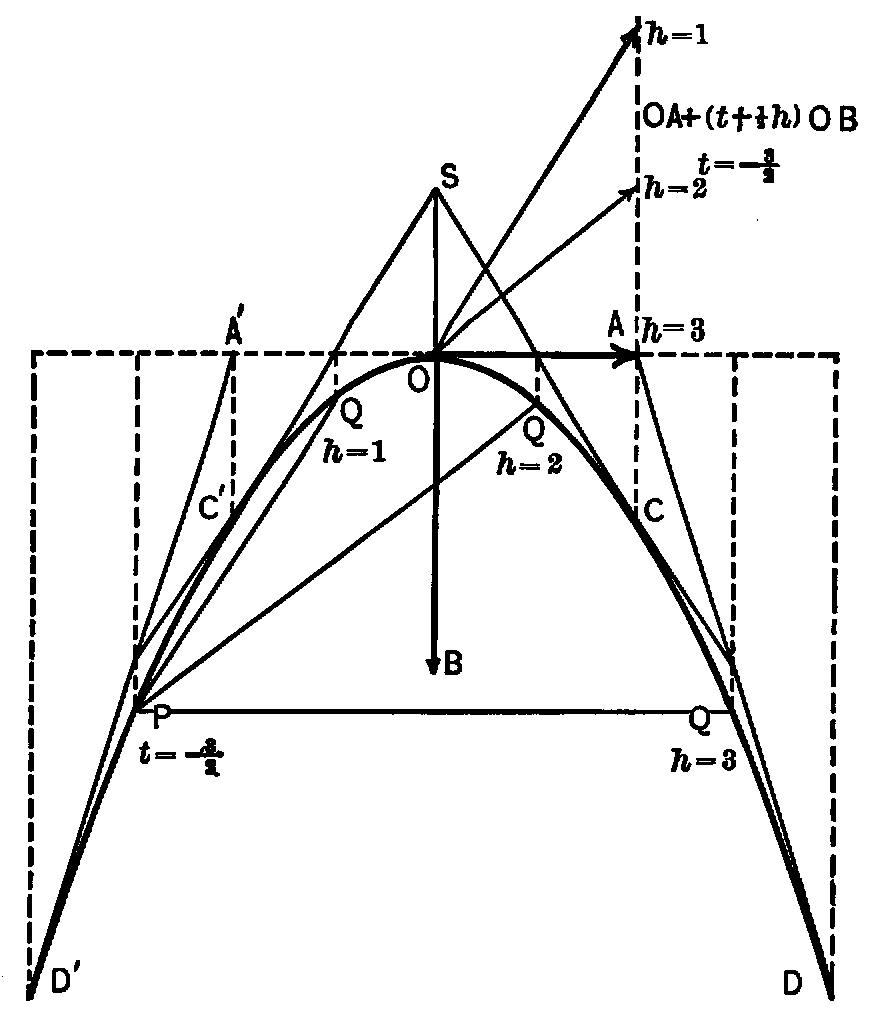
\includegraphics[width=80mm]{images/Image9.png}
\end{center}

(\textit{a}) To find the direction of the tangent to the locus at
the point $P$ corresponding to any value of $t$.

Let $P$, $Q$ be two points of the locus that correspond to the
values $t$, $t + h$ of the variable number. We have
\begin{gather*}
\mathbf{OP} = t\mathbf{OA} + \frac{1}{2} t^2 \mathbf{OB},\\
\mathbf{OQ} = (t + h) \mathbf{OA} + \frac{1}{2} (t + h)^2
\mathbf{OB},
\intertext{and therefore}
\mathbf{PQ} = \mathbf{OQ-OP} = h\left[\mathbf{OA} + (t + \frac{1}{2}
h)\mathbf{OB}\right].
\end{gather*}

Hence (dropping the factor $h$) we see that $\mathbf{OA} + (t +
\frac{1}{2} h) \mathbf{OB}$ is always \textit{parallel} to the
chord $PQ$. Make $h$ approach 0, and then $Q$ approaches $P$, and
the (indefinitely extended) chord $PQ$ approaches coincidence with
the tangent at $P$. Hence making $h = 0$, in the step that is
parallel to the chord, we find that $\mathbf{OA} + t\mathbf{OB}$
is parallel to the tangent at $P$.

Apply this result to the special positions of $P$ already found,
and we have: $\mathbf{D'A'} = \mathbf{OA - 2OB}=$
tangent at $D'$; $\mathbf{C'S = OA-OB} =$ tangent at
$C'$; $\mathbf{OA = OA + 0 \cdot OB =}$ tangent at $O$;
$\mathbf{SO = OA + OB =}$ tangent at $C$; $\mathbf{AD = OA +2 OB
=}$ tangent at $D$.

This is the curve described by a heavy particle thrown from $O$
with velocity represented by $\mathbf{OA}$ on the same scale in
which $\mathbf{OB}$ represents an acceleration of $32$
\textit{feet per second per second downwards}. For, after $t$
seconds the particle will be displaced a step $t \cdot
\mathbf{OA}$ due to its initial velocity, and a step
$\frac{1}{2}t^2\cdot \mathbf{OB}$ due to the acceleration
downwards, so that $P$ is actually the step $\mathbf{OP} =
t\mathbf{OA} + \frac{1}{2}t^2 \cdot \mathbf{OB}$ from $O$ at time
$t$. Similarly, since the velocity of $P$ is increased by a
velocity represented by $\mathbf{OB}$ in every second of time,
therefore $P$ is moving at time $t$ with velocity represented by
$\mathbf{OA} + t\mathbf{OB}$, so that this step must be parallel
to the tangent at $P$.

\item \textit{To draw the locus of a point $P$ that varies
according to the law}
\begin{equation*}
\mathbf{OP} = \cos (nt + e) \cdot \mathbf{OA} + \sin (nt + e)
\cdot \mathbf{OB},
\end{equation*}
\textit{where $\mathbf{OA,OB}$ are steps of equal length and
perpendicular to each other, and $t$ is any variable number.}

With centre $O$ and radius $OA$ draw the circle
$ABA'B'$. Take arc $AE=e$ radians in the direction
of the quadrant $AB$ (\textit{i.e.} an arc of $e$ radii of the
circle in length in the direction of $AB$ or $AB'$
according as $e$ is positive or negative). Corresponding to any
value of $t$, lay off arc $EP=nt$ radians in the direction of the
quadrant $AB$. Then arc $AP=nt+e$ radians. Draw $LP$ perpendicular
to $OA$ at $L$. Then according to the definitions of the
trigonometric functions of an angle we have,
\[
\cos(nt+e)=\overline{OL}/OP,\quad \sin(nt+e)=\overline{LP}/OP.
\footnote{Observe the distinctions: $\mathbf{OL}$, a step;
$\overline{OL}$, a positive or negative length of a directed axis;
$OL$, a length.}
\]
Hence we have for all values of $t$,
\begin{gather*}
\mathbf{OL}=\cos(nt+e) \mathbf{OA}, \quad \mathbf{LP}=\sin(nt+e)
\mathbf{OB},
\intertext{and adding these equations, we find that}
\mathbf{OP}=\cos(nt+e)\mathbf{OA}+\sin(nt+e)\mathbf{OB}.
\end{gather*}
Hence, \textit{the locus of the required point $P$ is the circle
on $\mathbf{OA, OB}$ as radii}.

\begin{center}
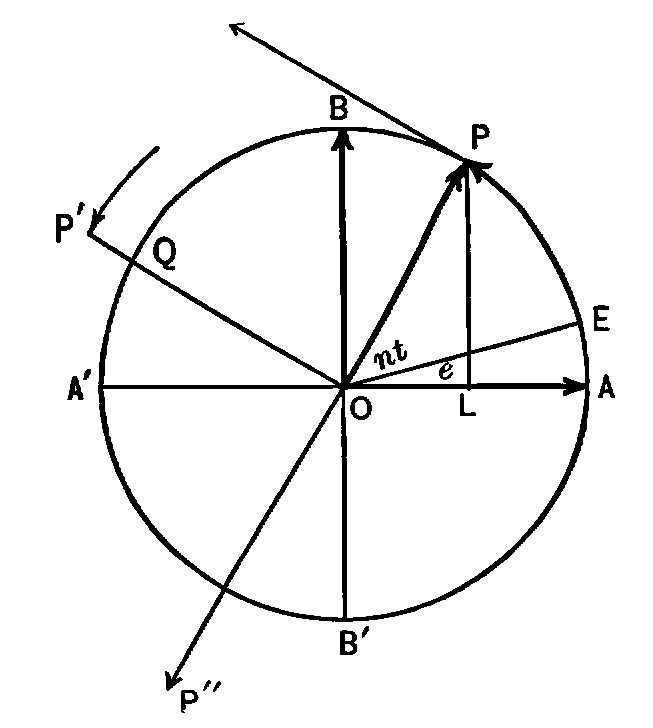
\includegraphics[width=80mm]{images/Image10.png}
\end{center}

Let $t$ be the number of seconds that have elapsed since epoch.
Then, at epoch, $t = 0$, and $P$ is at $E$; and since in $t$
seconds $P$ has moved through an arc $EP$ of $nt$ radians,
therefore $P$ moves uniformly round the circle at the rate of $n$
radians per second. Its velocity at time $t$ is therefore
represented by $n$ times that radius of the circle which is
perpendicular to $OP$ in the direction of its motion, or by
$\mathbf{OP'} = n\mathbf{OQ}$, where arc ${PQ} = \frac{\pi}{2}$
radians. Hence, since arc ${AQ}=(nt+e + \frac{\pi}{2})$ radians,
therefore $\mathbf{OP'} =n\left[\cos{\left(nt + e +
\frac{\pi}{2}\right)} \cdot \mathbf{OA} + \sin{\left(nt + e +
\frac{\pi}{2}\right)} \cdot \mathbf{OB}\right]$. The point $P\prime$ also
moves uniformly in a circle, and this circle is the hodograph of
the motion. The velocity in the hodograph (or the acceleration of
$P$) is similarly $\mathbf{OP''}= n^2\mathbf{PO}$.

\addcontentsline{toc}{section}{Parallel Projection}
\section*{Parallel Projection}

\item \textit{If $\mathbf{OP} = x\mathbf{OA} + y\mathbf{OB}$,
$\mathbf{OP'}=x\mathbf{OA} + y\mathbf{OB'}$, where $x$, $y$ vary
with the arbitrary number $t$ according to any given law so that
$P$, $P'$ describe definite loci (and have definite motions when $t$
denotes time), then the two loci (and motions) are parallel
projections of each other by rays that are parallel to $BB'$},

For, by subtracting the two equations we find $\mathbf{PP'} =
y\mathbf{BB'}$, so that $PP'$ is always parallel to $BB'$; and as $P$
moves in the plane $AOB$ and $P'$ moves in the plane $AOB'$, therefore
their loci (and motions) are parallel projections of each other by
rays parallel to $BB'$. The parallel projection is definite when
the two planes coincide, and may be regarded as a projection
between two planes $AOB$, $AOB'$, that make an indefinitely small
angle with each other.

\begin{center}
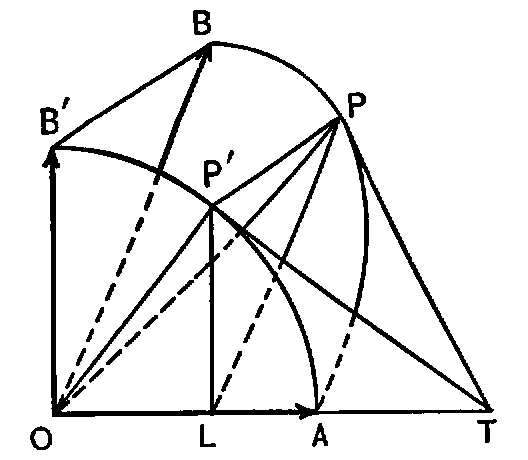
\includegraphics[width=80mm]{images/Image11.png}
\end{center}

\item \textit{The motion of $P$ that is determined by}
\begin{equation*}
\mathbf{OP} = \cos(nt + e)\mathbf{OA} + \sin(nt + e)\mathbf{OB}
\end{equation*}
\textit{is the parallel projection of uniform circular motion.}

For, draw a step $\mathbf{OB'}$ perpendicular to $\mathbf{OA}$ and
equal to it in length. Then, by Art.\ 18, the motion of $P'$
determined by
\begin{equation*}
\mathbf{OP'} = \cos(nt + e)\mathbf{OA} + \sin(nt + e)\mathbf{OB'}
\end{equation*}
is a uniform motion in a circle on $\mathbf{OA}$, $\mathbf{OB'}$
as radii; and by Art.\ 19 this is in parallel perspective with the
motion of $P$.

\addcontentsline{toc}{section}{Step Proportion}
\section*{Step Proportion}

\item \textsc{Definition.} \textit{Four steps} $\mathbf{AC}$,
$\mathbf{AB}$, $\mathbf{A'C'}$, $\mathbf{A'B'}$ \textit{are in
proportion when the first is to the second in respect to both
relative length and relative direction as the third is to the
fourth in the same respects.}

\begin{center}
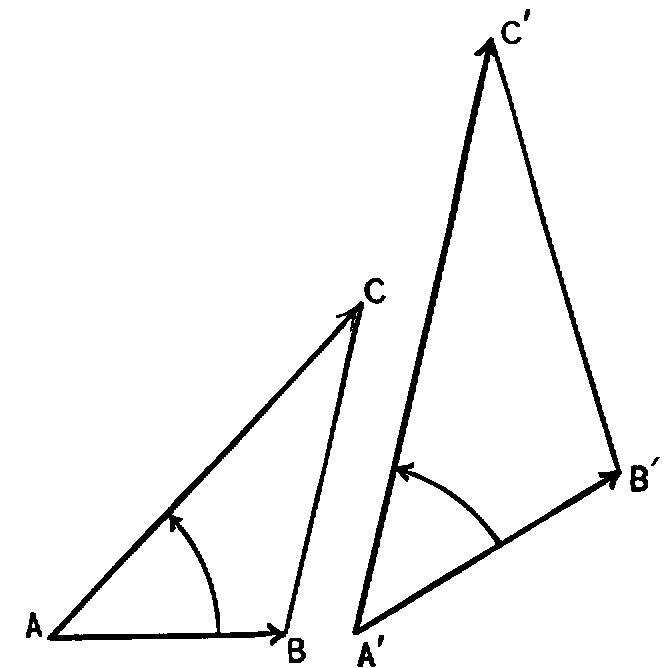
\includegraphics[width=80mm]{images/Image12.png}
\end{center}

This requires, first, that the lengths of the steps are in
proportion or
\begin{equation*}
AC: AB = A'C': A'B';
\end{equation*}
and secondly, that $\mathbf{AC}$ deviates from $\mathbf{AB}$ by
the same plane angle in direction and magnitude that
$\mathbf{A'C'}$ deviates from $\mathbf{A'B'}$.

Hence, first, the triangles $ABC$, $A'B'C'$ are similar, since the
angles $A$, $A'$ are equal and the sides about those angles are
proportional; and secondly, one triangle may be turned in its
plane into a position in which its sides lie in the same
directions as the corresponding sides of the other triangle. Two
such triangles will be called \textit{similar and congruent
triangles}, and corresponding angles will be called
\textit{congruent angles}.

\item We give the final propositions of Euclid, Book V., as
exercises in step proportion.

\begin{itemize}
\item (xi.) \textit{If four steps are proportionals, they are also
proportionals when taken alternately.}

\item (xii.) \textit{If any number of steps are proportionals,
then as one of the antecedents is to its consequent, so is the sum
of the antecedents to the sum of the consequents.}

\item (xiii.) \textit{If four steps are proportionals, the sum (or
difference) of the first and second is to the second as the sum
(or difference) of the third and fourth is to the fourth.}

\item (xiv.) If $\mathbf{OA:OB = OP:OQ}$ and $\mathbf{OB:OC =
OQ:OR}$,\\
then $\mathbf{OA:OC = OP:OR}$.

\item (xv.) If $\mathbf{OA:OB = OC:OD}$ and $\mathbf{OE:OB =
OF:OD}$,\\
then $\mathbf{OA+OE:OB = OC+OF:OD}$.

\item (xvi.) If $\mathbf{OA:OB = OB:OX = OC:OD =
OD:OY}$,\\
then $\mathbf{OA:OX = OC:IO}$.
\end{itemize}
\end{enumerate}

\addcontentsline{toc}{subsection}{Examples}
\subsection*{Examples}

\small We shall use $\mathbf{i}$, $\mathbf{j}$, $\mathbf{k}$, as
symbols for \textit{unit length east}, \textit{unit length north},
and \textit{unit length up}, respectively.

\begin{enumerate}
\item Mark the points whose steps from a given point are
$\mathbf{i}+2\mathbf{j}$, $-3\mathbf{i}-\mathbf{j}$. Show that the
step from the first point to the second is
$-4\mathbf{i}-3\mathbf{j}$, and that the length is 5.

\item Show that the four points whose steps from a given point are
$2\mathbf{i}+\mathbf{j}$, $5\mathbf{i}+4\mathbf{j}$,
$4\mathbf{i}+7\mathbf{j}$, $\mathbf{i}+4\mathbf{j}$ are the
angular points of a parallelogram. Also determine their centre of
gravity, with weights $1, 1, 1, 1$; also with weights $1, 2, 3, 4$;
also with weights $1, -2, 3, -4$.

\item If $\mathbf{OA} = \mathbf{i}+2\mathbf{j}$, $\mathbf{OB} =
4\mathbf{i}+3\mathbf{j}$, $\mathbf{OC} = 2\mathbf{i}+3\mathbf{j}$,
$\mathbf{OD}= 4\mathbf{i}+\mathbf{j}$, find $CD$ as sums of
multiples of $\mathbf{CA}$, $\mathbf{CB}$, and show that
$\mathbf{CD}$ bisects $\mathbf{AB}$.

\item If $\mathbf{OP} = x\mathbf{i}+y\mathbf{j}$, $\mathbf{OP'} =
x'\mathbf{i}+y'\mathbf{j}$, then $\mathbf{PP'} = (x'-x)\mathbf{i}
+ (y'-y)\mathbf{j}$ and ${\overline{PP'}}^2 = (x'-x)^2+(y'-y)^2$.

\item Show that $\mathbf{AB}$ is bisected by $\mathbf{OC =
OA+OB}$, and trisected by \linebreak $\mathbf{OD = 2OA+OB}$,
$\mathbf{OE = OA+2OB}$, and divided inversely as $2:3$ by
\linebreak $\mathbf{OF = 2OA+3OB}$.

\item Show that $\mathbf{AA'+BB' = 2MM'}$, where $MM'$ are the
middle points of $AB$, $A'B'$, respectively.

\item Show that $\mathbf{2AA'+3BB' = (2+3)CC'}$, where $C$, $C'$
are the points that divide $AB$, $A'B'$, inversely as $2:3$.
Similarly, when 2, 3 are replaced by $l$, $m$.

\item Show that the point that divides a triangle into three equal
triangles is the intersection of the medial lines of the triangle.

\item Show that the points which divide a triangle into triangles
of equal magnitude, one of which is negative (the given triangle
being positive), are the vertices of the circumscribing triangle
with sides parallel to the given triangle.

\item If $a$, $b$, $c$ are the lengths of the sides $BC$, $CA$,
$AB$ of a triangle, show that $\frac{1}{b}\mathbf{AC} \pm
\frac{1}{c}\mathbf{AB}$ (drawn from $A$) are interior and exterior
bisectors of the angle $A$; and that when produced they cut the
opposite side $BC$ in the ratio of the adjacent sides.

\item The $\left\lbrace
\begin{matrix}
  \text{lines} \\
  \text{points}
\end{matrix}\right.$ that join the $\left\lbrace
\begin{matrix}
  \text{vertices} \\
  \text{sides}
\end{matrix}\right.$ of a triangle $ABC$ to any $\left\lbrace
\begin{matrix}
  \text{point } P \\
  \text{line } p
\end{matrix}\right.$ in its plane divide the sides $BC$, $CA$,
$AB$ in ratios whose product is $\left\lbrace
\begin{matrix}
  +1 \\
  -1
\end{matrix}\right.$; and conversely $\left\lbrace
\begin{matrix}
  \text{lines from} \\
  \text{points on}\end{matrix}\right.$ the $\left\lbrace
\begin{matrix}
  \text{vertices} \\
  \text{sides}
\end{matrix}\right.$ that so divide the sides $\left\lbrace
\begin{matrix}
  \text{meet in a point.} \\
  \text{lie in a line.}\end{matrix}\right.$

\item Prove by Exs.\ 10, 11, that the three interior bisectors of
the angles of a triangle (also an interior and two exterior
bisectors) meet in a point; and that the three exterior bisectors
(also an exterior and two interior bisectors) meet the sides in
colinear points.

\item Determine the locus (and motion) of $P$, given by
$\mathbf{OP = OA}+t\mathbf{OB}$; also of $\mathbf{OP} =
(1+2t)\mathbf{i}+(3t-2)\mathbf{j}$.

\item Compare the loci of $P$ determined by the following
\textit{pairs} of \textbf{step} and \textbf{length} equations:
\begin{gather*}
\mathbf{AP} = 2\text{ east},\quad AP = 2; \qquad
  \mathbf{AP} = 2\mathbf{BP}, \quad AP = 2BP; \\
\mathbf{AP+BP = CD}, \quad  AP+BP = CD
\end{gather*}

\item Draw, by points and tangents, the locus of $P$ determined by
each of the following values of $\mathbf{OP}$, in which $x$ is any
number:
\begin{gather*}
x\mathbf{i}+\frac{1}{2}x^2\mathbf{j}; \quad
x\mathbf{i}+\frac{2}{x}\mathbf{j}; \quad
x\mathbf{i}+\frac{1}{3}x^3\mathbf{j}; \quad
x\mathbf{i}+(\frac{1}{3}x^3-x^2+2)\mathbf{j}; \\
x\mathbf{i}+\frac{8}{x^2+4}\mathbf{j}; \quad
x\mathbf{i}+\sqrt{4-x^2}\mathbf{j}; \quad
x\mathbf{i}+\frac{1}{2}\sqrt{4-x^2}\mathbf{j}.
\end{gather*}

\item Take three equal lengths making angles $120^{\circ}$ with each
other as projections of $\mathbf{i}$, $\mathbf{j}$, $\mathbf{k}$,
and construct by points the projection of the locus of $P$, where
$\mathbf{OP} = 2(\cos{x}{\cdot}\mathbf{i} +
\sin{x}{\cdot}\mathbf{j}) + x{\cdot}\mathbf{k}$, $x$ varying from
0 to $2\pi$. Show that this curve is one turn of a helix round a
vertical cylinder of altitude $2\pi$, the base being a horizontal
circle of radius 2 round $O$ as centre.

\item A circle rolls inside a fixed circle of twice its diameter;
show that any point of the plane of the rolling circle traces a
parallel projection of a circle.

\item A plane carries two pins that slide in two fixed rectangular
grooves; show that any point of the sliding plane traces a
parallel projection of a circle.

\item $OACB$ is a parallelogram whose sides are rigid and jointed
so as to turn round the vertices of the parallelogram; $APC$,
$BCQ$ are rigid similar and congruent triangles. Show that
$\mathbf{AC:AP = BQ:BC = OQ:OP}$, and that therefore $P$, $Q$
trace similar congruent figures when $O$ remains stationary (21,
22, xii.). [See cover of book.]

\item If the plane pencil $OA$, $OB$, $OC$, $OD$ is cut by any
straight line in the points $P$, $Q$, $B$, $S$, show that the
\textit{cross-ratio}
$(\overline{PR}:\overline{RQ}) : (\overline{PS}:\overline{SQ})$ is
constant for all positions of the line.
\begin{equation*}
[\mathbf{OC} = l\mathbf{OA}+m\mathbf{OB} = lx\mathbf{OP}+ my\mathbf{OQ}
  \text{ gives } \overline{PR}:\overline{RQ} = my:lx].
\end{equation*}

\item Two roads run north, and east, intersecting at $O$. $A$ is
60 \textit{feet south} of $O$, walking 3 \textit{feet per second
north}, $B$ is 60 \textit{feet west} of $O$, walking 4
\textit{feet per second east}. When are $A$, $B$ nearest together,
and what is $B$'s apparent motion as seen by $A$?

\item What is $B$'s motion relative to $A$ in Ex.\ 21 if $B$ is
accelerating his walk at the rate of 3 \textit{inches per second
per second}?

\item In Ex.\ 21, let the east road be 20 feet above the level of
the north road; and similarly in Ex.\ 22.

\item A massless ring $P$ is attached to several elastic strings
that pass respectively through smooth rings at $A$, $B$, $C$,
$\cdots$ and are attached to fixed points $A'$, $B'$, $C'$,
$\cdots$ such that $A'A$, $B'B$, $C'C$, $\cdots$ are the natural
lengths of the strings. The first string has a tension $l$ per
unit of length that it is stretched (Hooke's law), the second a
tension $m$, the third a tension $n$, etc. Find the resultant
force on $P$ and its position of equilibrium.

\item The same as Ex.\ 24, except that the ring has a mass $w$.
\end{enumerate} \normalsize

\newpage
\chapter{Rotations. Turns. Arc Steps}

\addcontentsline{toc}{section}{Definitions and Theorems of
Rotation}

\begin{enumerate}
\setcounter{enumi}{22}
\item \textsc{Definitions of Rotation}

A step is \textbf{rotated} when it is revolved about an axis through its
initial point as a rigid length rigidly attached to the axis. The
step describes a conical angle about the axis except when it is
perpendicular to the axis.

\begin{center}
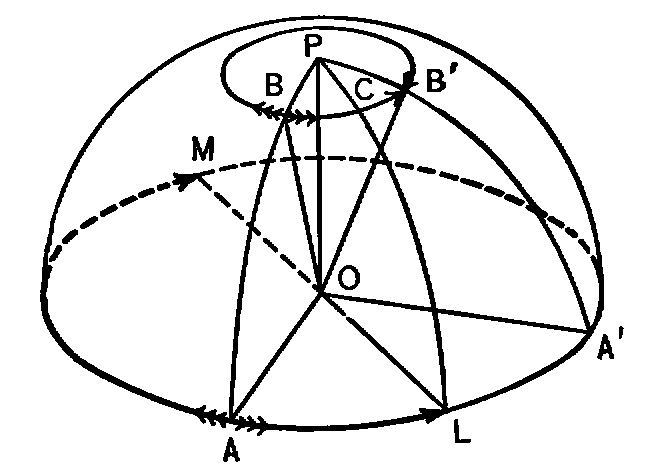
\includegraphics[width=80mm]{images/Image13.png}
\end{center}

If a rotation through a diedral angle of given magnitude and
direction in space be applied to the radii of a sphere of unit
radius and centre $O$, the sphere is rotated as a rigid body about
a certain diameter $PP'$ as axis, and a plane through $O$
perpendicular to the axis intersects the sphere in the
\textbf{equator} of the rotation.

Either of the two directed arcs of the equator from the initial
position $A$ to the final position $A'$ of a point of the rotated
sphere that lies on the equator is the \textbf{arc} of the
rotation. If these two arcs he bisected at $L$, $M$ respectively,
then the two arcs are $2\overset\frown{AL}$, $2\overset\frown{AM}$
respectively, and $\overset\frown{AL}$, $\overset\frown{AM}$ are
supplementary arcs in opposite directions, each less than a
semicircle. When these half-arcs are $0^{\circ}$ and $180^{\circ}$
respectively, they represent a rotation of the sphere into its
original position, whose axis and equator are indeterminate, so
that such arcs may be measured on any great circle of the sphere
without altering the corresponding rotation.

\item \textit{A rotation is determined by the position into which
it rotates two given non-parallel steps.}

For let the radii $\mathbf{OB}$, $\mathbf{OC}$ rotate into the
radii $\mathbf{OB'}$, $\mathbf{OC'}$. Any axis round which
$\mathbf{OB}$ rotates into $\mathbf{OB'}$ must be equally inclined
to these radii; \textit{i.e.}, it is a diameter of the great
circle $PKL$ that bisects the great arc $\overset\frown{BB'}$ at
right angles.

\begin{center}
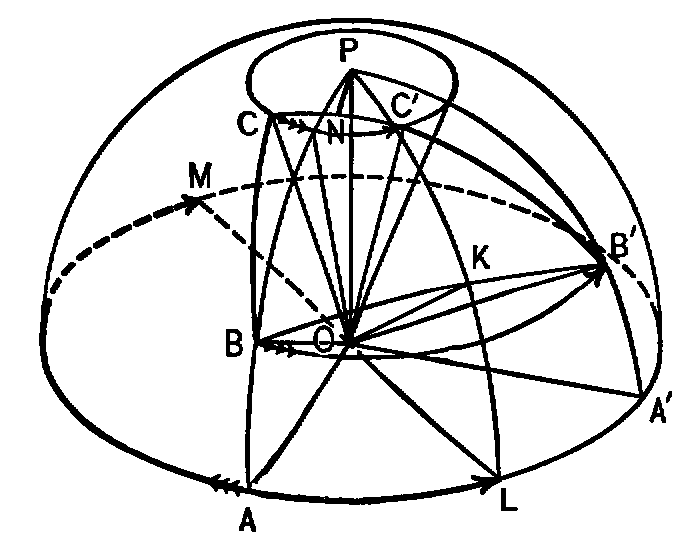
\includegraphics[width=80mm]{images/Image14.png}
\end{center}

\textit{E.g.}, $OK$, $OL$, $OP$, $\cdots$ are such axes.
Similarly, the axis that rotates $\mathbf{OC}$ into $\mathbf{OC'}$
must be a diameter of the great circle $PN$ that bisects the great
arc $\overset\frown{CC'}$ at right angles. Hence there is but
one axis round which $\mathbf{OB}$, $\mathbf{OC}$ rotate into
$\mathbf{OB'}$, $\mathbf{OC'}$; viz., the intersection $OP$ of the
planes of these two bisecting great circles: the equator is the
great circle whose plane is perpendicular to this axis, and the
arcs of the rotation are the intercepts on the equator by the
planes through the axis and either $B$, $B'$ or $C$, $C'$. [When
the two bisecting great circles coincide (as when $C$, $C'$ lie on
$BP$, $B'P$), then their plane bisects the diedral angle
$BC-O-B'C'$, whose edge $OP$ is the only axis of rotation.]

\small \textsc{Note.} Since $\overset\frown{BC}$,
$\overset\frown{B'C'}$ may be any two positions of a marked arc on
the surface of the sphere, we see that any two positions of the
sphere with centre fixed determine a definite rotation of the
sphere from one position to the other. \normalsize

\item \textit{A marked arc of a great circle of a rotating sphere
makes a constant angle with the equator of the rotation.}

For the plane of the great arc makes a constant angle both with
the axis and with the equator of the rotation.

\item \textit{If the sphere $O$ be given a rotation
$2\overset\frown{A_0C}$ followed by a rotation
$2\overset\frown{CB_0}$, the resultant rotation of the sphere is
$2\overset\frown{A_0B_0}$.}

\begin{center}
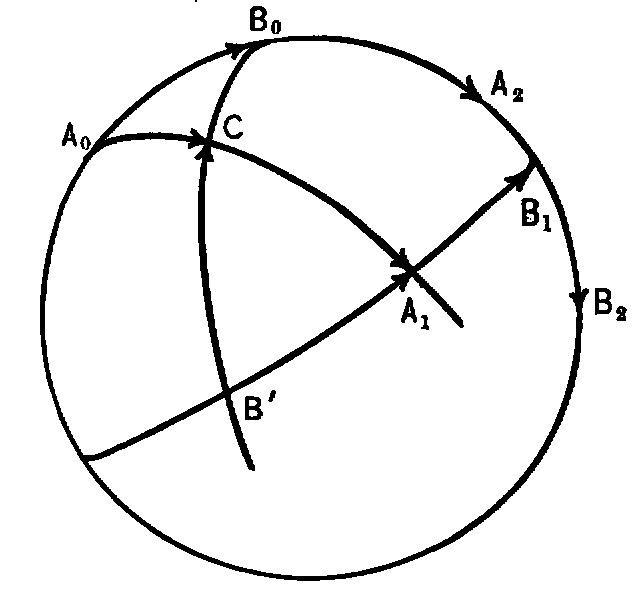
\includegraphics[width=80mm]{images/Image15.png}
\end{center}

For produce the arcs $\overset\frown{A_0C}$,
$\overset\frown{B_0C}$ to $A_1$, $B'$ respectively, making
$\overset\frown{CA_1} = \overset\frown{A_0C}$,
$\overset\frown{B'C} = \overset\frown{CB_0}$. Then the spherical
triangles $A_0B_0C$, $A_1B'C$ are equal, since the corresponding
sides about the equal vertical angles at $C$ are by construction
equal. Therefore the sides $\overset\frown{A_0B_0}$,
$\overset\frown{B'A_1}$ are equal in length, and the corresponding
angles $A_0$, $A_1$ and $B_0$, $B'$ are equal. Therefore, by Art.\
25, if a marked arc $\overset\frown{AB}$ of the sphere coincide
initially with $\overset\frown{A_0B_0}$, the first rotation
$2\overset\frown{A_0C} = \overset\frown{A_0A_1}$ will bring
$\overset\frown{AB}$ into the position $\overset\frown{A_1B_1}$ on
$\overset\frown{B'A_1}$ produced, and the second rotation
$2\overset\frown{CB_0} = \overset\frown{B'B_1}$ will bring
$\overset\frown{AB}$ into the position $\overset\frown{A_2B_2}$ on
$\overset\frown{A_0B_0}$ produced, where $\overset\frown{B_0A_2}$
= $\overset\frown{A_0B_0}$. Hence the resultant rotation of the
sphere is $2\overset\frown{A_0B_0}$ = $\overset\frown{A_0A_2}$.

\small \textsc{Note.} This theorem enables one to find the
resultant of any number of successive rotations, by replacing any
two successive rotations by their resultant, and so on until a
single resultant is found. \normalsize

\addcontentsline{toc}{section}{Definitions of Turn and Arc Steps}
\item \textsc{Definitions of Turn}

A step is turned when it is made to describe a \textit{plane
angle} round its initial point as centre.

\begin{center}
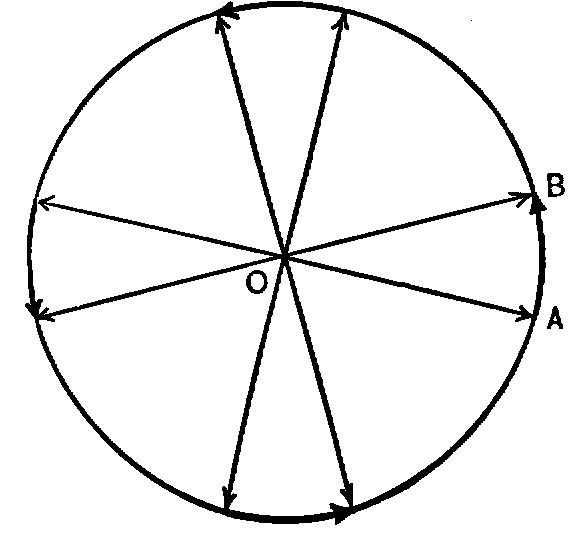
\includegraphics[width=80mm]{images/Image16.png}
\end{center}

If a turn through a plane angle of given magnitude and direction
in space be applied to the radii of the sphere $O$, it turns the
great circle that is parallel to the given plane angle as a rigid
circle, and does not affect the other radii of the sphere.
\textit{E.g.}, only horizontal radii can be turned through a
horizontal plane angle. The circle that is so turned is the great
circle of the turn.

A directed arc of the great circle of a turn from the initial
position $A$ to the final position $B$ of a point on the great
circle, and less than a semi-circumference, is the arc of the
turn. When this arc is $0^{\circ}$ or $180^{\circ}$, it represents
a turn that brings a step back to its original position or that
reverses it; and since such turns may take place in any plane with
the same results, therefore such arcs may be measured on any great
circle of the sphere without altering their corresponding turns.

The \textbf{axis} of a turn is that radius of the sphere $O$ which
is perpendicular to its great circle and lies on that side of the
great circle from which the arc of the turn appears
counter-clockwise.

\item \textit{A turn is determined by the position into which it
displaces any given step.}

For, let the radius $\mathbf{OA}$ turn into the radius
$\mathbf{OB}$. Then, the great circle $O-AB$ must be the great
circle of the turn, and $\overset\frown{AB}$, the arc of the turn.

\item \textsc{Definitions.} The resultant of two successive turns
$\overset\frown{AB}$, $\overset\frown{BC}$ is the turn
$\overset\frown{AC}$.

\begin{center}
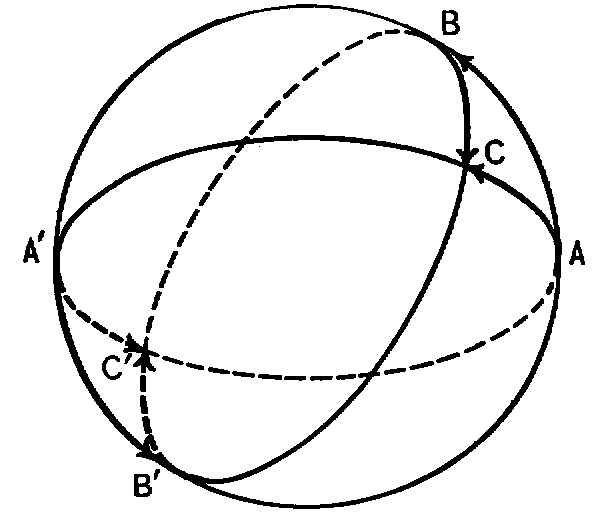
\includegraphics[width=80mm]{images/Image17.png}
\end{center}

When the arc of the turns are not given with the first ending
where the second begins, each arc may be moved as a rigid arc
round its great circle until they do so end and begin, without
altering their turning value. When the two great circles are not
the same, then the common point of the two arcs must be one or the
other point of intersection $(B, B')$ of the two great circles.
The figure shows that the same resultant is found from either of
these points.

\subsubsection{ARC STEPS}

We may call the great arc $\overset\frown{AB}$ the \textbf{arc
step} from $A$ to $B$ on the surface of the sphere; and call two
arc steps \textbf{equal} when they are arcs of the same great
circle of the same length and direction; and call
$\overset\frown{AC}$ the \textbf{sum} of $\overset\frown{AB}$,
$\overset\frown{BC}$ or the sum of any arc steps equal to these.
The half-arc of a resultant rotation is thus the sum of the
half-arcs of its components, and the arc of a resultant turn is
the sum of the arcs of the components. The sum of several arcs is
found by replacing any two successive arcs of the sum by their
sum, and so on, until a single sum is found. An arc of $0^{\circ}$
or $180^{\circ}$ may be measured on any great circle without
altering its value as the representative of a half-rotation, a
turn, or an arc step.

\item \textit{The resultant of two successive rotations or turns
(i.e., the sum of two arc steps) is commutative only when the arcs
are cocircular.}

For let the half-arcs of the rotations, or the arcs of the turns,
be $\overset\frown{AB} = \overset\frown{BA'}$, and
$\overset\frown{C'B} = \overset\frown{BC}$; then the sums
$\overset\frown{AB}+\overset\frown{BC}$,
$\overset\frown{C'B}+\overset\frown{BA'}$ in opposite orders are
respectively $\overset\frown{AC}$, $\overset\frown{C'A'}$; and
from the figure those arcs are equal when, and only when, the
given arcs are cocircular.

\begin{center}
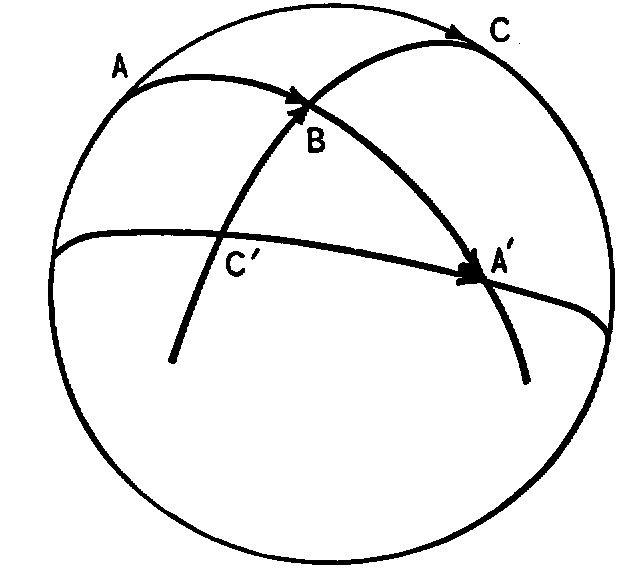
\includegraphics[width=80mm]{images/Image18.png}
\end{center}

\begin{itemize}
\item \textsc{Cor.\ 1.} \textit{An arc of $0^{\circ}$ or
$180^{\circ}$ is commutative with any other arc.}

For it may be taken cocircular with the other arc.

\item \textsc{Cor.\ 2.} \textit{The magnitudes of the sums of two
arcs in opposite orders are equal.}

For $ABC$, $A'BC'$ are equal spherical triangles by construction,
and therefore $\overset\frown{AC}$, $\overset\frown{C'A'}$ are
equal in length.
\end{itemize}

\item \textit{A sum of successive arc steps is associative.}

\begin{center}
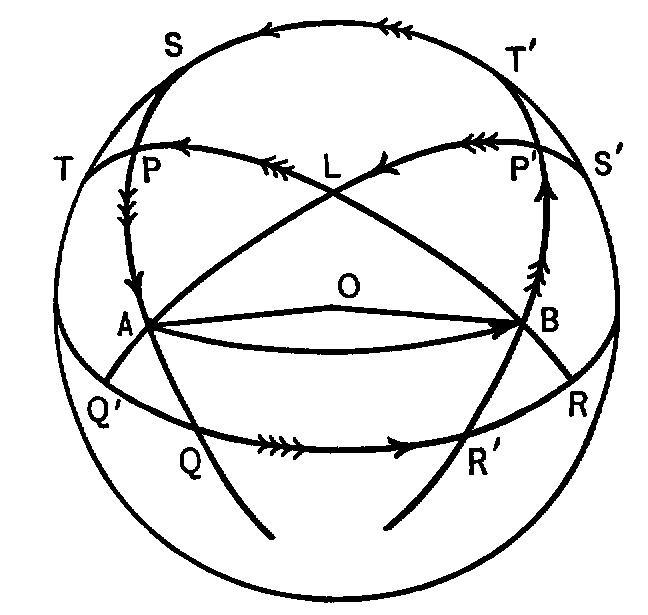
\includegraphics[width=80mm]{images/Image19.png}
\end{center}

For, consider first three arcs upon the great circles $LQ'$,
$Q'R$, $RL$. If the arcs are such as to begin and end
successively, the proof is the same as for step addition,
\textit{e.g.}, in the sum $\overset\frown{AQ'} +
\overset\frown{Q'R} + \overset\frown{RB} = \overset\frown{AB}$,
the first two may be replaced by their sum $\overset\frown{AR}$,
or the second and third by their sum $\overset\frown{Q'B}$ without
altering the whole sum. In the more general case when the three
arcs are
\begin{equation*}
\overset\frown{AQ'} = \overset\frown{S'P'}, \quad
\overset\frown{Q'Q} = \overset\frown{R'R}, \quad
\overset\frown{RB} = \overset\frown{PT},
\end{equation*}
the sum of the first two is $\overset\frown{AQ} =
\overset\frown{SP}$, whose sum with the third is
$\overset\frown{ST}$; and the sum of the second and third is
$\overset\frown{R'B} = \overset\frown{P'T'}$, whose sum with the
first is $\overset\frown{S'T'}$; and we must prove that
$\overset\frown{ST}$, $\overset\frown{S'T'}$ are equal arcs of the
same great circle in the same direction.

\smallskip
[Observe that in the construction $P$ is determined as the
intersection of $QA$ and $RB$, and $P'$ as the intersection of
$Q'A$ and $R'B$.]

\smallskip
Let the three given arcs be the half-arcs of successive rotations
of the sphere $O$. Then by Art.\ 26, the rotation
$2\overset\frown{AQ} = 2\overset\frown{SP}$ gives the sphere the
same displacement as the first and second rotations, so that
$2\overset\frown{ST}$ gives the sphere the same displacement as
the three rotations. Similarly, the rotation $2\overset\frown{R'B}
= 2\overset\frown{P'T}$ gives the sphere the same displacement as
the second and third rotations, so that $2\overset\frown{S'T'}$
gives the sphere the same displacement as the three rotations.
Hence $\overset\frown{ST}$, $\overset\frown{S'T'}$ are arcs of the
same great circle, and either equal (and in the same direction) or
supplementary (and in opposite directions), since they are
half-arcs of the same rotation. This is true wherever $Q$ may be.
Suppose that $Q$ is slightly displaced towards $R$; then
$\overset\frown{ST}$, $\overset\frown{S'T'}$ are slightly
displaced, and if equal at first, they must remain equal, since a
slight change in each of two equal arcs could not change them to
supplementary arcs in opposite directions.\footnote{When both arcs
are nearly $90^{\circ}$, a slight change in each could change them
from equals to supplements in the same direction.} Hence by moving
$Q$ continuously towards $R$ and finding how the arcs
$\overset\frown{ST}$, $\overset\frown{S'T'}$ are related when $Q$
reaches $R$, we find how they are related for any position of $Q$,
since there is no change in the relation when $Q$ is moved
continuously. But when $Q$ is at $R$, it was shown above that both
arcs were equal; therefore $\overset\frown{ST}$,
$\overset\frown{S'T'}$ are always equal.

\smallskip
So, in general, for a sum of any number of successive arcs, any
way of forming the sum by replacing any two successive terms by
their sum and so on, must give a half-arc of the resultant of the
rotations through double each of the given arcs. Hence any two
such sums are either equal or opposite supplementary arcs of the
same great circle; and since by continuous changes of the
component arcs, they may be brought so that each begins where the
preceding arc ends, in which position the two sums are equal,
therefore they are always equal.

\begin{itemize}
\item \textsc{Cor.\ 1.} \textit{An arc of $0^{\circ}$ or
$180^{\circ}$ may have any position in a sum.} [Art.\ 30, Cor.\ 1.]

\item \textsc{Cor.\ 2.} \textit{The magnitude of a sum of arcs is
not changed by a cyclic change in the order of its terms.}

For $(\overset\frown{AB} + \overset\frown{CD} + \cdots) +
\overset\frown{HK}$ and $\overset\frown{HK} + (\overset\frown{AB}
+ \overset\frown{CD} + \cdots)$ have equal magnitudes. [Art.\ 30,
Cor.\ 2.]
\end{itemize}
\end{enumerate}

\addcontentsline{toc}{subsection}{Examples}
\subsection*{EXAMPLES}

\small \begin{enumerate}

\item Show that $2(\overset\frown{AB} + \overset\frown{BC})$ and
$2\overset\frown{AB} + 2\overset\frown{BC}$ are in general
unequal.

\item If (2, $30^{\circ}$) denote a turn of $30^{\circ}$
counter-clockwise in the plane of the paper and a doubling, and
(3, $-60^{\circ}$) denote a turn of $60^{\circ}$ clockwise in the
plane of the paper and a trebling, express the resultant of these
two compound operations (\textit{versi-tensors}) in the same
notation.

\item Find the resultant of (2, $30^{\circ}$), (3, $60^{\circ}$),
(4, $-120^{\circ}$), (1, $180^{\circ}$).

\item Show that either (2, $-60^{\circ}$) or (2, $120^{\circ}$)
taken twice have the resultant (4, $-120^{\circ}$).

\item Would you consider the resultants of \textit{versi-tensors}
as their sums or their products, and why?

\item Let the base $QR$ of a spherical triangle $PQR$ slide as a
rigid arc round its fixed great circle, and let the great circles
$QP$, $RP$, always pass through fixed points $A$, $B$
respectively. Show that if points $S$, $T$ lie on the great
circles $QP$, $RP$ so as always to keep $\overset\frown{PS} =
\overset\frown{QA}$ and $\overset\frown{PT} = \overset\frown{RB}$,
then the arc $\overset\frown{ST}$ is an arc of fixed length and
direction that slides around a fixed great circle as
$\overset\frown{QR}$ slides round its fixed great circle. [Let
$P'$, $Q'$, $R'$, $S'$, $T'$, be given positions of $P$, $Q$, $R$,
$S$, $T$, and use Art.\ 31 and figure.]

\item Show that the locus of the radius $OP$ in Ex.\ 6 is an
oblique circular cone of which $OA$, $OB$ are two elements, and
that the fixed great circles $QR$, $ST$ are parallel to its
circular sections. [Draw a fixed plane parallel to $OQR$ and
cutting the radii $OA$, $OB$, in the fixed points $A'$, $B'$, and
cutting $OP$ in the variable point $P'$, and show that $P'$
describes a circle in this plane through the fixed points $A'$,
$B'$; similarly, for a fixed plane parallel to $OST$.]

\textsc{Note.}---The locus of $P$ on the surface of the sphere is
called a \textbf{spherical conic} (the intersection of a sphere
about the vertex of a circular cone as centre with the surface of
the cone); and the great circles $QR$, $ST$ (parallel to the
circular sections of the cone) are the \textit{cyclic} great
circles of the spherical conic. The above properties of a
spherical conic and its cyclic great circles become properties of
a plane conic and its \textit{asymptotes} when the centre $O$ of
the sphere is taken at an indefinitely great distance.

\item State and prove Ex.\ 6 for a plane, and construct the locus
of $P$.
\end{enumerate} \normalsize

\newpage
\chapter{Quaternions}

\addcontentsline{toc}{section}{Definitions and Theorem}

\begin{enumerate}
\setcounter{enumi}{31}
\item \textsc{Definitions.} A \textbf{quaternion} is a number that
alters a step in length and direction by a given ratio of
extension and a given turn. \textit{E.g.}, in the notation of Ex.\
2, II, (2, $30^{\circ}$), (2, $-60^{\circ}$) are quaternions.

Two quaternions are \textbf{equal} when, and only when, their
ratios of extension are equal and their turns are equal.

A \textbf{tensor} is a quaternion that extends only;
\textit{i.e.}, a tensor is an ordinary positive number. Its turn
is $0^{\circ}$ in any plane.

A \textbf{versor} or \textbf{unit} is a quaternion that turns
only. \textit{E.g.}, $1$, $-1 = (1, 180^{\circ})$, $(1,
90^{\circ})$, $(1, 30^{\circ})$, are versors.

A \textbf{scalar} is a quaternion whose product lies on the same
line or ``scale'' as the multiplicand; \textit{i.e.}, a scalar is an
ordinary positive or negative number. Its turn is $0^{\circ}$ or
$180^{\circ}$ in any plane.

A \textbf{vector} is a quaternion that turns $90^{\circ}$.
\textit{E.g.}, $(2, 90^{\circ})$, $(1,-90^{\circ})$, are vectors.

\item \textsc{Functions of a Quaternion} $q$. The \textbf{tensor}
of $q$, or briefly $Tq$, is its ratio of extension. \textit{E.g.},
$T2 = 2 = T(-2) = T(2, 30^{\circ})$.

The \textbf{versor} of $q$ ($Uq$) is the versor with the same arc
of turn as $q$. \textit{E.g.},
\begin{equation*}
U2 = 1, \quad U(-2) = -1, \quad U(2, 30^{\circ}) = (1, 30^{\circ}).
\end{equation*}

The \textbf{arc, angle, axis, great circle,} and \textbf{plane} of
$q$, are respectively the \textit{arc, angular magnitude, axis,
great circle,} and \textit{plane} of its turn. \textit{E.g.},
$\mathrm{arc } (2, 30^{\circ})$ is a counter-clockwise arc of
$30^{\circ}$ of unit radius in the plane of the paper, and
$\mathrm{arc } (2, -30^{\circ})$ is the same arc oppositely
directed; $\angle(2, 30^{\circ}) = \angle(2,-30^{\circ}) =
30^{\circ} = \frac{\pi}{6} \mathrm{ radians}$; $\mathrm{axis }(2,
30^\circ)$ is a unit length perpendicular to the plane of the
paper directed towards the reader, and $\mathrm{axis }(2,
-30^{\circ})$ is the same length oppositely directed; etc.

\begin{center}
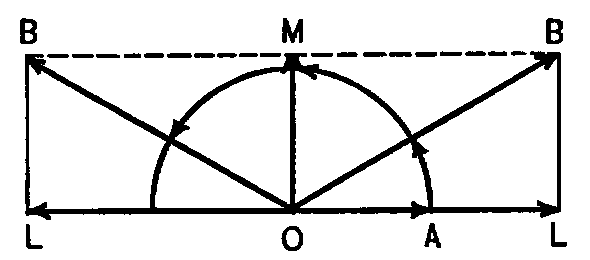
\includegraphics[width=80mm]{images/Image20.png}
\end{center}

If $q\mathbf{OA} = \mathbf{OB}$, and if $L$ be the foot of the
perpendicular from $B$ upon the line $OA$, then $\mathbf{OL}$,
$\mathbf{LB}$ are called \textit{the components of $q$'s product}
\textit{respectively parallel and perpendicular to the
multiplicand;} also, \textit{the projections of $\mathbf{OB}$
parallel and perpendicular to $\mathbf{OA}$.}

The \textbf{scalar} of $q$ ($Sq$) is the scalar whose product
equals the component of $q$'s product parallel to the
multiplicand; \textit{viz.}, $Sq\cdot\mathbf{OA} = \mathbf{OL}$.

\textit{E.g.}, $S(2, 30^{\circ}) = \sqrt{3}, \quad
S(2, 150^{\circ}) = -\sqrt{3}$.

The \textbf{vector} of $q$ ($Vq$) is the vector whose product
equals the component of $q$'s product perpendicular to the
multiplicand; \textit{viz.}, $Vq\cdot\mathbf{OA} = \mathbf{LB}$.

\textit{E.g.}, $V(2, 30^{\circ}) = (1, 90^{\circ})= V(2, 150^{\circ}),
\quad V(2, -60^{\circ}) = (\sqrt{3}, -90^{\circ})$.

The \textbf{reciprocal} of $q$ ($1/q$ or $q^{-1}$) is the
quaternion with reciprocal tensor and reversed turn.
\textit{E.g.}, $(2, 30^{\circ})^{-1}=(\frac{1}{2},-30^{\circ})$.

The \textbf{conjugate} of $q(Kq)$ is the quaternion with the same
tensor and reversed turn. \textit{E.g.,}
\begin{equation*}
K(2,30^{\circ}) = (2,-30^{\circ}).
\end{equation*}

\item From the above diagram and the definitions of the cosine and
sine of an angle, we have
\begin{gather}
\tag{a} Sq = \frac{\mathbf{OL}}{\mathbf{OA}} = \frac{\overline{OL}}{OA} =
  \frac{OB}{OA} \cdot \frac{\overline{OL}}{OB} = Tq \cdot \cos\angle{q} \\
\tag{b} TVq = \frac{LB}{OA} = \frac{OB}{OA} \cdot \frac{LB}{OB} =
  Tq \cdot \sin\angle{q}
\end{gather}

\small \textsc{Note.} \textit{Arc $Vq$ is a quadrant on the great
circle of $q$ in the direction of arc $q$.} \normalsize
\end{enumerate}

\addcontentsline{toc}{subsection}{Examples}
\subsection*{Examples}

\small \begin{enumerate}
\item If equal numbers multiply equal steps, the products are
equal; and if they multiply unequal steps, the products are
unequal.

\item If the products of two steps by equal numbers are equal,
then the two steps are equal; and if the products of two equal
steps by two numbers are equal, then the numbers are equal.

\item If several steps be multiplied by equal numbers, then any
product is to its multiplicand as any other product is to its
multiplicand.

\item If two steps be multiplied by reciprocal numbers, then
corresponding products and multiplicands are reciprocally
proportional.

\item Construct the following products, where $\mathbf{OA}$ is a
unit step to the right in the plane of the paper, and determine
the functions of each multiplier that are defined in Art.\ 33.

\begin{enumerate}
\item $2\cdot\mathbf{OA = OL}$, \quad
$(4, 60^{\circ})\cdot\mathbf{OA = OB}$, \quad
$(4,-60^{\circ})\cdot\mathbf{OA = OB'}$, \\
$(2\sqrt{3},90^{\circ})\cdot\mathbf{OA = OM}$, \quad
$(2\sqrt{3},-90^{\circ})\cdot\mathbf{OA = OM'}$, \\
$(1, 60^{\circ})\cdot\mathbf{OA = OB_1}$, \quad
$(1,-60^{\circ})\cdot\mathbf{OA = OB_1'}$, \\
$(1, 90^{\circ})\cdot\mathbf{OA = OM_1}$, \quad
$(1,-90^{\circ})\cdot\mathbf{OA = OM_1'}$.

\item The same as (a) with $120^{\circ}$ in the place of
$60^{\circ}$.
\end{enumerate}

\item Show that $SSq = Sq$, \quad $SVq = 0$, \quad $VSq = 0$,
\quad $VVq = Vq$, \\ $SKq = KSq = Sq$, \quad $VKq = KVq$, \quad
$USq = \pm 1$, \quad $UTq = 1 = TUq$.
\end{enumerate} \normalsize

\addcontentsline{toc}{section}{Multiplication}
\section*{Multiplication}

\begin{enumerate}
\setcounter{enumi}{34}
\item \textsc{Definition.} The \textbf{product} of two or more
numbers is that number whose extension and turn are the resultants
of the successive extensions and turns of the factors (beginning
with the right-hand factor).

\textit{E.g.}, if $r\mathbf{OA = OB}$, $q\mathbf{OB = OC}$,
$p\mathbf{OC = OD}$, then we have $pqr\cdot\mathbf{OA} =
pq\mathbf{OB} = p\mathbf{OC} = \mathbf{OD}$.

\item The product is, however, independent of whether a step
$\mathbf{OA}$ can be found or not, such that each factor operates
upon the product of the preceding factor; \textit{i.e.}, we have
by definition,

(\textit{a}) $T(\cdots pqr) = \cdots Tp \cdot Tq \cdot Tr$.

(\textit{b}) $\text{arc }(\cdots pqr) = \text{arc }r + \text{arc
}q + \text{arc }p + \cdots$.

\item \textit{The product of a tensor and a versor is a number
with that tensor and versor; and conversely, a number is the
product of its tensor and its versor.}

For if $n$ be a tensor, and $q'$ a versor, then $nq'$ turns by the
factor $q'$ and extends by the factor $n$, and \textit{vice versa}
for $q'n$; hence either of the products, $nq'$, $q'n$, is a
quaternion with tensor $n$ and versor $q\prime$. Similarly,
\begin{equation*}
q = Tq \cdot Uq = Uq \cdot Tq.
\end{equation*}

\item \textit{Any successive factors of a product may be replaced
by their product without altering the value of the whole product;
but in general such factors can be changed in order without
altering the value of the product only when those factors are
cocircular.}

For replacing successive factors by their product does not alter
the tensor of the whole product by Art.\ 36(a), nor the arc of the
product by Art.\ 31, 36(b); but by Art.\ 30 the arc of the product
is altered if two factors be interchanged except when those
factors are cocircular.

\begin{itemize}
\item \textsc{Cor.\ 1.} \textit{A scalar factor may have any
position in the product without altering the value of the
product.} [Art.\ 31, Cor.\ 1.]

\item \textsc{Cor.\ 2.} \textit{The angle of a product is not
altered by a cyclic change in the order of the factors.} [Art.\
31, Cor.\ 2.]

\item \textsc{Cor.\ 3.} \textit{The scalar, and the tensor of the
vector, of a product are not altered by a cyclic change in the
order of the factors.} [Art.\ 34, \textit{a, b}.]
\end{itemize}

\item \textit{The product of two numbers with opposite turns
equals the product of the tensors of the numbers; and conversely
if the product of two numbers is a tensor, then the turns of the
factors are opposites.} [36 \textit{a, b}.]

\begin{itemize}
\item \textsc{Cor.\ 1.} \textit{The product of two conjugate
numbers equals the square of their tensor; and if the product of
two numbers with equal tensors is a tensor, then the two numbers
are conjugates.}

\item \textsc{Cor.\ 2.} \textit{The conjugate of a product equals
the product of the conjugates of the factors in reverse order.}

For $(pqr)(Kr\cdot Kq\cdot Kp) = (Tp)^2 \cdot (Tq)^2 \cdot (Tr)^2$
since $rKr = (Tr)^2$, may have any place in the product, and may
be put first; and then $(qKq) = (Tq)^2$, may be put second, and
then $(pKp) = (Tp)^2$. [Cor.\ 1, 38 Cor.\ 1.]

Hence, $K(pqr) = Kr \cdot Kq \cdot Kp$. [Cor.\ 1.]

\item \textsc{Cor.\ 3.} \textit{The product of two reciprocal
numbers is unity; and conversely, if the product of two numbers
with reciprocal tensors is unity, then the numbers are
reciprocals.}

\item \textsc{Cor. 4.} \textit{The reciprocal of a product equals
the product of the reciprocals of the factors in reverse order.}

For $(pqr)(r^{-1}q^{-1}p^{-1}) = 1$.
\end{itemize}

\item \textit{The square of a vector is $-1$ times the square of
its tensor; and conversely, if the square of a number is a
negative scalar, then the number is a vector.} [36, \textit{a, b}.]

\begin{itemize}
\item \textsc{Cor.\ 1.} \textit{The conjugate of a vector is the
negative vector.} [39 Cor.\ 1.]

\item \textsc{Cor.\ 2.} \textit{The conjugate of a product of two
vectors is the product of the same vectors in reverse order.}
[Art.\ 39, Cor.\ 2.]

\item \textsc{Cor.\ 3.} \textit{The conjugate of a product of
three vectors is the negative of the product of the same vectors
in reverse order.} [Art.\ 39, Cor.\ 2.]
\end{itemize}

\addcontentsline{toc}{section}{The Rotator $q()q^{-1}$}
\section*{The Rotator $q()q^{-1}$}

\item We may consider the ratio of two steps as determining a
number, the antecedent being the product and the consequent the
multiplicand of the number; \textit{viz.}, ${\mathbf OB/OA}$
determines the number $r$ such that $r{\mathbf OA = OB}$. By Art.\
21, equal step ratios determine equal numbers.

If the several pairs of steps that are in a given ratio $r$ be
given a rotation whose equatorial arc is $2\text{ arc }q$, they
are still equal ratios in their new positions and determine a new
number $r'$ that is called \textit{the number $r$ rotated through
$2\text{ arc }q$.} In other words, the rotation of $r$ produces a
number with the same tensor as $r$, and whose great circle and arc
are the rotated great circle and arc of $r$.

\item \textit{The number $r$ rotated through $2\text{ arc }q$ is
the number $qrq^{-1}$.}

For, 1st, $Tqrq^{-1} = Tq \cdot Tr(Tq)^{-1} = Tr$.

\begin{center}
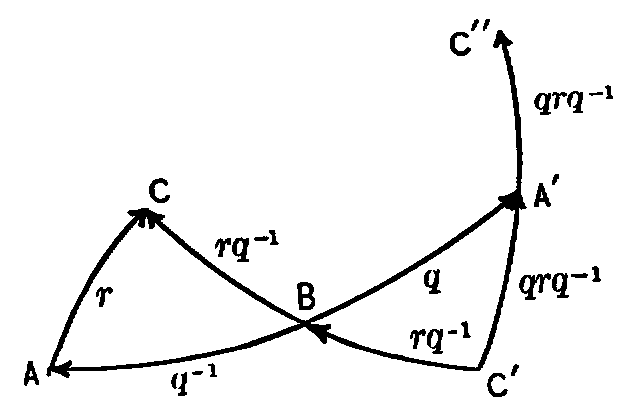
\includegraphics[width=80mm]{images/Image21.png}
\end{center}

2d, let $A$ be an intersection of the great circle of $r$ with the
great circle of $q$ and construct
\begin{gather*}
\overset\frown{AB} = \overset\frown{BA^{\prime}} = \text{arc }q, \quad
\overset\frown{AC} = \text{arc }r,
\intertext{and}
\overset\frown{C'B} = \overset\frown{BC} = \text{arc }rq^{-1};
\intertext{then}
\overset\frown{C'A'} = \overset\frown{A'C''} = \text{arc }qrq^{-1}.
\end{gather*}
But by construction, the spherical triangles $ABC$, $A'BC'$ are
equal, and therefore $\overset\frown{AC}$ and
$\overset\frown{C'A'} ( = \overset\frown{A'C''})$ are arcs of
equal length, and the corresponding angles at $A$, $A'$ are equal.
Hence, when arc $r ( = \overset\frown{AC})$ is rotated through
$2\text{ arc }q( = \overset\frown{AA'})$, it becomes arc
$qrq^{-1}( = \overset\frown{A'C''})$.

\addcontentsline{toc}{section}{Powers and Roots}
\section*{Powers and Roots}

\item An integral power, $q^n = q \cdot q \cdot q \cdots$ \textit{to
n factors}, is determined by the equations,

\begin{enumerate}
\item $T \cdot q^n = Tq \cdot Tq \cdot Tq \cdots  = (Tq)^n$.

\item $\text{arc }q^n = \text{arc }q + \text{arc }q + \text{arc }q
\cdots = n \text{ arc }q \pm (\text{whole circumferences})$.

To find $q^{\frac{1}{n}}$, \textit{the number whose $n$th power is
$q$}, we have, by replacing $q$ by $q^{\frac{1}{n}}$ in
(\textit{a}), (\textit{b}),

\item $Tq = (T \cdot q^{\frac{1}{n}})^n$ or
$T \cdot q^{\frac{1}{n}} = (Tq)^{\frac{1}{n}}$

\item $\text{Arc }q = n\text{ arc }q^{\frac{1}{n}} \pm$ whole
circumferences, or, arc $q^{\frac{1}{n}} = {\frac{1}{n}}$
(arc $q \pm$ whole circumferences) $= {\frac{1}{n}}$ arc $q
+ {\frac{m}{n}}$ circumferences $\pm$ whole circumferences),
where $m = 0,\,1,\,2,\,3,\,\cdots\, n-1$, successively.
\end{enumerate}

There are therefore $n$ $n$th roots of $q$ whose tensors are all
equal and whose arcs lie on the great circle of $q$.

When the base is a scalar, its great circle may be any great
circle, so that there are an infinite number of quaternion $n$th
roots of a scalar. On this account, the roots as well as the
powers of a scalar are \textbf{limited to scalars.} By ordinary
algebra, there are $n$ such $n$th roots, real and imaginary. There
are also imaginary $n$th roots of $q$ besides the $n$ real roots
found above; \textit{i.e.}, roots of the form $a+b\sqrt{-1}$,
where $a$, $b$ are real quaternions.

\addcontentsline{toc}{section}{Representation of Vectors}
\section*{Representation of Vectors}

\item Bold-face letters will be used as symbols of vectors only.
In particular, $\mathbf{i}$, $\mathbf{j}$, $\mathbf{k}$ will
denote \textit{unit} vectors whose axes are respectively a unit
length east, a unit length north, and a unit length up. More
generally we shall use the step $\mathbf{AB}$ to denote the vector
whose axis is a unit length in the direction of $\mathbf{AB}$, and
whose tensor is the numerical length of $\mathbf{AB}$ ($= AB$:
{\textit unit length}).

This use of a step $\mathbf{AB}$ as the symbol of a vector is
analogous to the use of $AB$ to represent a tensor ($AB$: {\textit
unit length}), or of $\overline{AB}$ to represent a positive or
negative scalar, according as it is measured in or against the
direction of its axis of measurement. In none of these cases is
the concrete quantity an absolute number; {\textit i.e.}, the
value of the number that it represents varies with the assumed
unit of length. When desirable, we distinguish between the vector
$\mathbf{OA}$ and the step $\mathbf{OA}$ by enclosing the vector
in a parenthesis.

\item {\it If $q(\mathbf{OA}) = (\mathbf{OB})$, then
$q \cdot \mathbf{OA} = \mathbf{OB}$, and conversely.}

The tensor of $q$ in either equation is $OB:OA$. It is therefore
only necessary to show that the arc of $q$ in one equation equals
the arc of $q$ in the other equation in order to identify the two
numbers that are determined by these two equations as one and the
same number.

\begin{center}
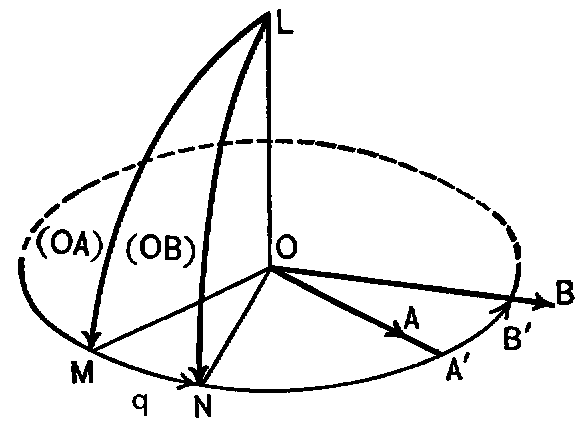
\includegraphics[width=80mm]{images/Image22.png}
\end{center}

Draw the sphere of unit radius and centre $O$, cutting
$\mathbf{OA}$, $\mathbf{OB}$ in $A'$, $B'$; then
$\overset\frown{A'B'}$ is the arc of $q$ in the second equation.
Draw the radius $OL$ perpendicular to the plane $OA'B'$ on the
counter-clockwise side of $\overset\frown{A'B'}$, and draw
counter-clockwise round $OA'$, $OB'$ as axes the quadrants
$\overset\frown{LM}$, $\overset\frown{LN}$ respectively; then
these are the arcs of $(\mathbf{OA})$, $(\mathbf{OB})$
respectively, and since $\overset\frown{LM} + \overset\frown{MN} =
\overset\frown{LN}$, therefore $\overset\frown{MN}$ is the arc of
$q$ in the first equation. But since $\overset\frown{LM}$,
$\overset\frown{LN}$ are quadrants, therefore the plane $OMN$ is
perpendicular to $OL$, and must therefore coincide with the plane
$OA'B'$, which is by construction also perpendicular to $OL$.
Hence $\overset\frown{MN}$ lies on the great circle of
$\overset\frown{A'B'}$, and by the construction of the figure, it
must, when advanced $90^{\circ}$ on that great circle, coincide
with $\overset\frown{A'B'}$. Hence the theorem.

\small \textsc{Note}. This theorem shows that a number extends and
turns vectors into vectors in the same way that it extends and
turns steps into steps. Moreover, when the vector is not
perpendicular to the axis of the multiplier, there is no resulting
vector, since in the case of the corresponding step there is no
resulting step. In the case of a vector multiplicand, that is
oblique to the axis of $q$, the product is an actual quaternion
that is not a vector, while in the case of the corresponding step
multiplicand the product belongs to that class of products in
which the multiplicand does not admit of the operation of the
multiplier, as in \textit{$\sqrt{2}$ universities, -2 countries,
etc}. \normalsize

\begin{itemize}
\item \textsc{Cor.\ 1.} \textit{The product of two vectors is a
vector when, and only when, the factors are perpendicular to each
other; the product is perpendicular to both factors; and its
length (its tensor) is equal to the area of the rectangle on the
lengths of the factors.}

\small \textsc{Note}. The direction of the product $\mathbf{OA}
\cdot \mathbf{OB = OC}$ is obtained by turning $\mathbf{OB}$ about
$\mathbf{OA}$ as axis through a counter-clockwise right angle;
thus $\mathbf{OC}$ lies on that side of the plane $OAB$ from which
the right angle $AOB$ appears counter-clockwise. \normalsize

\item \textsc{Cor.\ 2.} \textit{The product of two perpendicular
vectors changes sign when the factors are interchanged.}
($\mathbf{OB}\cdot \mathbf{OA = OC' = -OC}$.)

\begin{center}
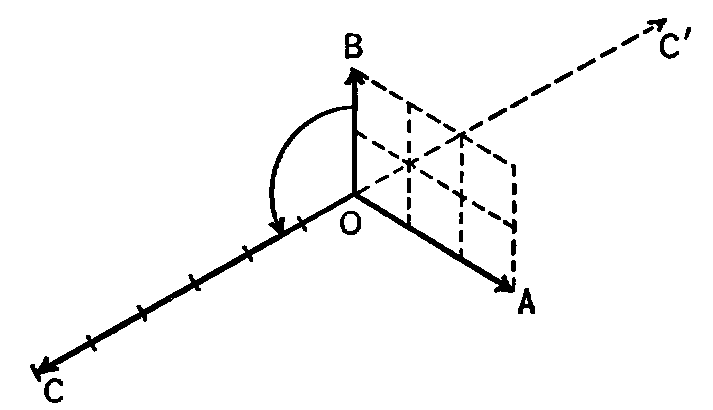
\includegraphics[width=80mm]{images/Image23.png}
\end{center}

\item \textsc{Cor.\ 3.} \textit{The condition that $\alpha$ is
perpendicular to $\beta$ is that $\alpha\beta = $ vector, or
$S\alpha\beta = 0$}.
\end{itemize}

\item \textit{If $\mathbf{AB}$, $\mathbf{CD}$ are parallel, then
$\mathbf{AB \cdot CD = CD \cdot AB} = -\overline{AB} \cdot
\overline{CD}$, a scalar; and conversely, the product of two
vectors is a scalar only when they are parallel.}

Since the axes of the vectors $\mathbf{AB}$, $\mathbf{CD}$ are
parallel, therefore their product is commutative. When the vectors
are in the same direction, then each turns $90^{\circ}$ in the same
direction, the resultant turn is $180^{\circ}$, and the product is
negative; and when the vectors are in opposite direction, their
turns are in opposite directions, the resultant turn is $0^{\circ}$,
and the product is positive. This is just the opposite of the
product of the corresponding scalars $\overline{AB}$,
$\overline{CD}$, which is positive when the scalars are in the
same direction (or both of the same sign), and negative when the
scalars are in opposite directions; \textit{i.e.},
$\mathbf{AB{\cdot}CD} = -\overline{AB}\cdot\overline{CD}$.

Conversely, the product $\mathbf{AB}$, $\mathbf{CD}$ can be a
scalar only when the resultant of their two turns of $90^{\circ}$
each is a turn of $0^{\circ}$ or $180^{\circ}$; \textit{i.e.},
only when the turns are cocircular, and therefore their axes
parallel.

\begin{itemize}
\item \textsc{Cor.} \textit{The condition that $\alpha$ is parallel to
$\beta$ is $\alpha\beta =$ scalar, or $V\alpha\beta = 0$}.
\end{itemize}
\end{enumerate}

\addcontentsline{toc}{subsection}{Examples}
\subsection*{Examples}

\small \begin{enumerate}
\item Prove by diagram that $(pq)^2$ and $p^2q^2$ are in general
unequal.

\item Find the 2d, 3d, 4th, 5th, 6th powers of $(2, 90^{\circ})$,
$(2, -60^{\circ})$.

\item Find the square roots and cube roots of $(4, 30^{\circ}),
(8, -120^{\circ})$.

\begin{enumerate}
\item Find the values of $[(2, 50^{\circ})^6]^\frac{1}{3}$, $[(2,
50^{\circ})^\frac{1}{3}]^{6}$, and $(2, 50^{\circ})^\frac{6}{3}$.
\end{enumerate}

\item What numbers are represented by 2 \textit{feet}, 2
\textit{feet east}, the unit of length being a foot, a yard, an
inch?

\item Show that $\mathbf{i^2 = j^2 = k^2 = ijk = -1}$; $\mathbf{jk
= i = -kj}$; $\mathbf{ki = j = -ik}$; $\mathbf{ij = k = -ji}$.

\item Let $e^\mathbf{(AB)}$ denote the versor that turns
counter-clockwise round the axis $AB$ through an arc that is
formed by bending the length AB into an arc of unit radius. Show
that if facing the west, and holding the paper in a north and
south vertical plane, then $e^\mathbf{i}$, $e^\mathbf{2i}$,
${\cdots}e^\mathbf{-i}$, $e^\mathbf{-2i}$, turn respectively 1, 2,
$\cdots$ radians counter-clockwise, and 1, 2, $\cdots$ radians
clockwise in the plane of the paper. Also show that
$e^{\pm\frac{\pi}{2}\mathbf{i}} = \pm\mathbf{i}$,
$e^{\pm\pi\mathbf{i}} = -1$ $e^{2n\pi\mathbf{i}} = 1$, where $n$
is any integer.

\item Show by diagram that $Se^{\theta\mathbf{i}} = \cos\theta$,
$Ve^{\theta\mathbf{i}} = i\sin\theta$, where $\theta$ is any
positive or negative number and the unit of angle is a radian.

\item Show that if $\mathbf{OA}$ rotate into $\mathbf{OB}$ through
$2\text{ arc }q$, then $(\mathbf{OB}) = q(\mathbf{OA})q^{-1}$.

\item Show that if $\alpha$ be a vector in the plane of $q$, then
$Kq = \alpha{q}\alpha^{-1} = \alpha^{-1}q\alpha$.

\item Show that $pq$ rotates into $qp$, and determine two such
rotations.

\item Show that $SKq = Sq$, $VKq = -Vq$.

\item Show that $K\alpha\beta = \beta\alpha$, $S\alpha\beta =
S\beta\alpha$, $V\alpha\beta = -V\beta\alpha$.

\item Show that $K\alpha\beta\gamma = -\gamma\beta\alpha$;
$V\alpha\beta\gamma = V\gamma\beta\alpha$; $S\alpha\beta\gamma =
S\beta\gamma\alpha = S\gamma\alpha\beta = -S\gamma\beta\alpha =
-S\beta\alpha\gamma = -S\alpha\gamma\beta$. (\textit{a}) Determine the
conjugate of a product of $n$ vectors.

\item Prove by diagram that $Kpq = Kq \cdot Kp$.
\end{enumerate} \normalsize

\addcontentsline{toc}{section}{Addition}
\section*{Addition}

\begin{enumerate}
\setcounter{enumi}{46}

\item \textsc{Definition}. The sum $(p+q)$ is the number
determined by the condition that its product is the sum of the
products of $p$ and $q$.

\begin{center}
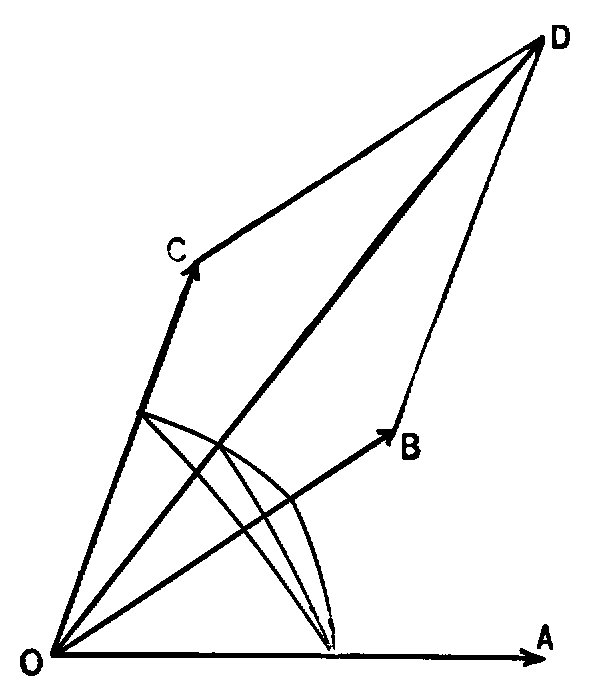
\includegraphics[width=80mm]{images/Image24.png}
\end{center}

Thus let $\mathbf{OA}$ be any step that is multiplied by both $p$
and $q$, and let $p\mathbf{OA = OB}$, $q\mathbf{OA = OC}$, and
$\mathbf{OB + OC = OD}$, then $(p+q)\mathbf{OA = OD}$. It is
obvious that any change in $\mathbf{OA}$ alters $\mathbf{OB}$,
$\mathbf{OC}$, $\mathbf{OD}$, proportionally, so that the value of
the sum $p+q(= \mathbf{OD:OA})$ is the same for all possible
values of $\mathbf{OA}$.

Similarly, any quaternion, $r$, may be added to the sum $p+q$,
giving the sum $(p+q)+r$; and we may form other sums such as
$p+(q+r)$, $(q+r)+p$, etc. It will be shown later that all such
sums of the same numbers are equal, or that quaternion addition is
\textit{associative} and \textit{commutative}.

\item \textit{The sum of a scalar and a vector is a quaternion
with that scalar and that vector, and conversely, a quaternion is
the sum of its scalar and its vector.}

\begin{center}
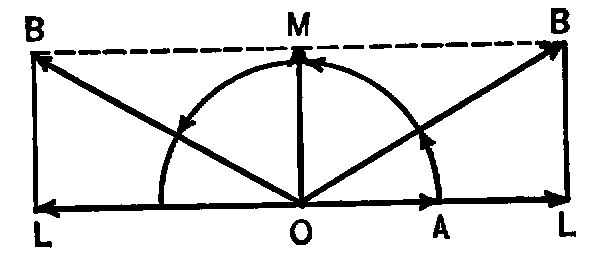
\includegraphics[width=80mm]{images/Image25.png}
\end{center}

For let $w$ be any scalar, and $\rho$ any vector, and let
$w\mathbf{OA} = \mathbf{OL}$, \linebreak[4] $\rho\mathbf{OA =
OM}$, then completing the rectangle $\mathbf{OLBM}$, we have
\newline $(w + \rho)\mathbf{OA = OB}$, and the scalar of $w+\rho$
is $w$, and its vector is $\rho$, since $\mathbf{OL}$,
$\mathbf{OM}$ are the components of $\mathbf{OB}$ parallel and
perpendicular to $\mathbf{OA}$. Similarly,
\begin{equation*}
q = Sq+Vq.
\end{equation*}

\item \textit{The scalar, vector, and conjugate, of any sum equals
the like sum of the scalars, vectors, and conjugates of the terms
of the sum.} [\textit{I.e., $S$, $V$, $K$, are distributive over a
sum.}]

\begin{center}
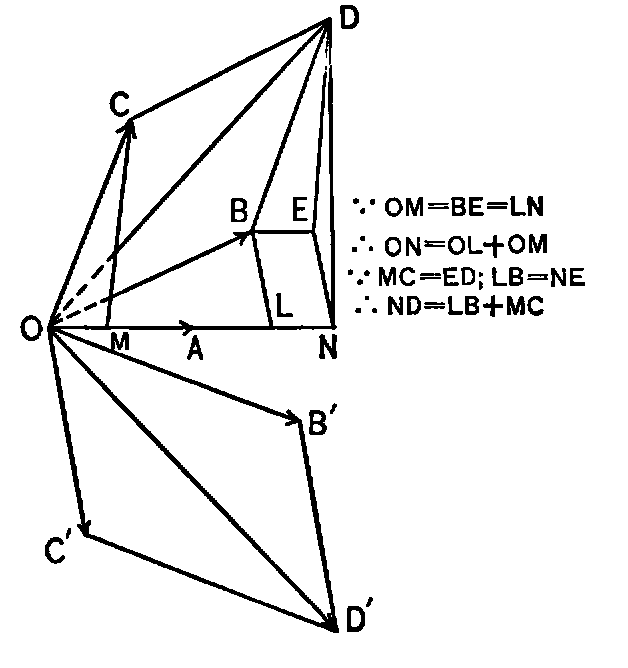
\includegraphics[width=80mm]{images/Image26.png}
\end{center}

For let
\begin{gather*}
p\mathbf{OA} = \mathbf{OB}, \quad q\mathbf{OA = OC}, \\
(p+q) \mathbf{OA} = \mathbf{OB + OC} = \mathbf{OD}.
\end{gather*}
Then the components of $\mathbf{OD}$ parallel and perpendicular to
$\mathbf{OA}$ are, by the figure, the sums of the like components
of $\mathbf{OB}$, $\mathbf{OC}$; \textit{i.e.}, $S(p+q) \cdot
\mathbf{OA} = Sp \cdot \mathbf{OA} + Sq \cdot \mathbf{OA}$, or
$S(p+q) = Sp+Sq$; and $V(p+q) \cdot \mathbf{OA} = Vp \cdot
\mathbf{OA} + Vq \cdot \mathbf{OA}$, or $V(p+q) = Vp+Vq$.

Also, if $OB'D'C'$ be the parallelogram that is symmetric to the
parallelogram $OBDC$ with reference to $OA$ as axis of symmetry,
then \linebreak $Kp \cdot \mathbf{OA = OB'}$, $Kq \cdot
\mathbf{OA = OC'}$, and $K(p+q) \cdot \mathbf{OA = OD'}$, and
since \linebreak $\mathbf{OB'+OC' = OD'}$, therefore $K(p+q) =
Kp + Kq$.

These results extend to any given sum; \textit{e.g.},
$V[(p+q)+r] = V(p+q)+Vr = (Vp+Vq)+Vr$, etc.

\item \textit{If $\mathbf{(OA)+(OB) = (OC)}$, then $\mathbf{OA +
OB = OC}$, and conversely.}

\begin{center}
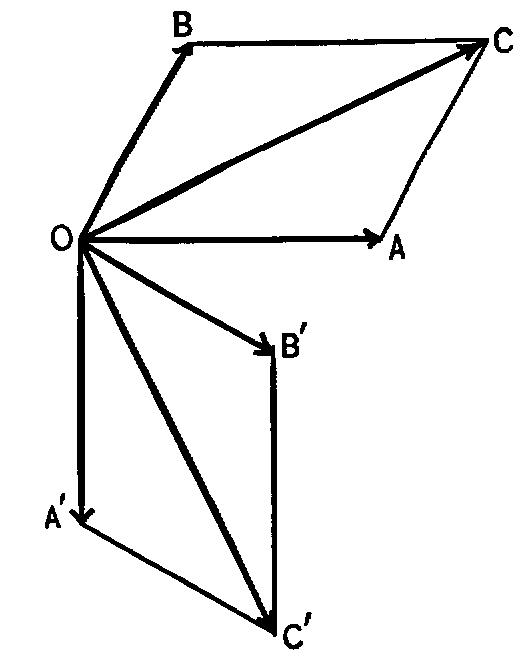
\includegraphics[width=80mm]{images/Image27.png}
\end{center}

For erect a pin $OD$ of unit length perpendicular to the plane of
the angle $AOB$ on its counter-clockwise side; and turn $AOB$
round $OD$ as axis through a clockwise right angle as seen from
$D$ into the position $A'OB'$. Then since $({\mathbf OA})$ is the
vector that turns through a counter-clockwise right angle round
$OA$ as axis, and extends unit length into $OA = OA'$, therefore
${\mathbf (OA)OD = OA'}$, and similarly ${\mathbf (OB)OD = OB'}$,
and therefore ${\mathbf (OC)OD = OA'+OB' = OC'}$, where $OA'C'B'$
is a parallelogram. Hence the step ${\mathbf OC}$ of proper length
and direction to give the tensor and axis of the vector ${\mathbf
(OC)}$ must be the diagonal of the parallelogram on ${\mathbf
OA}$, ${\mathbf OB}$ as sides; and therefore ${\mathbf OA+OB =
OC}$. Conversely, if ${\mathbf OA+OB = OC}$, then turning the
parallelogram $OACB$ into the position $OA'C'B'$, we have, since
${\mathbf OA'+OB' = OC'}$, that ${\mathbf (OA)+(OB) = (OC)}$.

\begin{itemize}
\item \textsc{Cor.\ 1.} \textit{Vectors add in the same way as
their corresponding steps, and all the laws of addition and
resolution of steps extend at once to vectors.}

\item \textsc{Cor.\ 2.} \textit{A sum of quaternions is
associative and commutative.}
\end{itemize}

For since by Cor.\ 1 a sum of vectors is independent of the way in
which its terms are added, and since we know that a sum of scalars
(i.e., ordinary numbers) is independent of the way in which its
terms are added, therefore by Art.\ 49 the scalar and the vector of
a sum are independent of the way in which the sum is added. Hence
the sum is independent of the way in which it is added, since it
is equal to the sum of its scalar and its vector.

\item \textsc{Lemma.} \textit{If $p$, $q$ be any quaternions, then
$(1+p)q = q+pq$.}

\begin{center}
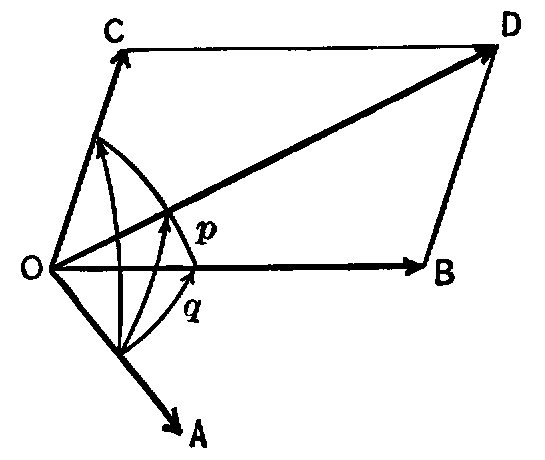
\includegraphics[width=80mm]{images/Image28.png}
\end{center}

For take $\mathbf{OB}$ in the intersection of the planes of $p$,
$q$ and draw $\mathbf{OA}$, $\mathbf{OC}$ such that
$q \cdot \mathbf{OA = OB}$, $p\mathbf{OB = OC}$; then
$(1+p)q \cdot \mathbf{OA} = (1+p)\mathbf{OB} = \mathbf{OB+OC} =
q\mathbf{OA} + pq\mathbf{OA}$. Hence,
\begin{equation*}
(1+p)q=q+pq.
\end{equation*}

\item \textit{If $p$, $q$, $r$ be any quaternions, then $(p+q)r =
pr+qr$.}

For we have, $(1+qp^{-1})p \cdot r = (1+qp^{-1}) \cdot pr$, and
expanding each member by the preceding lemma, we have, $(p+q)r =
pr+qr$.

This result extends to any sum; \textit{e.g.},
\begin{equation*}
(p+q+r+s)t = [(p+q)+(r+s)]t = (p+q)t+(r+s)t = pt+qt+rt+st.
\end{equation*}

\begin{itemize}
\item \textsc{Cor.\ 1.} $r(p+q) = rp+rq$.

For let $p'$, $q'$, $r'$ be the conjugates of $p$, $q$, $r$. Then
from $(p'+q')r' = p'r'+q'r'$, we have, by taking the conjugates of
each member, $r(p+q) = rp+rq$. [Art.\ 39, Cor.\ 2; Art.\ 49.]

\item \textsc{Cor.\ 2.} \textit{A product of sums equals the sum
of all partial products that may be formed from the given product
by multiplying together, in the order in which they stand, a term
from each factor of the product.}

\textit{E.g., $(p+q)(r+s) = pr+ps+qr+qs$.}
\end{itemize}

\small \textsc{Note}.---This rule should be used even when the
factors are commutative, as it prevents all danger of taking out
the same partial product twice; \textit{e.g.}, from taking both
$pr$ and $rp$ from the above product. To be sure that all the
partial products are found, some system of arrangement should be
adopted; also the total number of partial products should be
determined. \normalsize

\textit{E.g.}, $(p+q)(p+q)(p+q)$ may be arranged according to the
degrees of the terms in $p$, and there are $2\times2\times2 = 8$
terms. This product is then easily seen to be
\begin{gather*}
p^3+(p^2q+pqp+qp^2)+(pq^2+qpq+q^2p)+q^3,
\intertext{when $p$, $q$ are not commutative, and}
p^3+3p^2q+3pq^2+q^3,
\end{gather*}
when $p$, $q$ are commutative.

\addcontentsline{toc}{section}{Formulas}
\section*{Formulas. For Exercise and Reference}

\item \begin{enumerate} \item $q = Tq \cdot Uq = Uq \cdot Tq$.

\item $q = Sq+Vq$; $Kq = Sq-Vq$.

\item $Sq = Tq\cos\angle{q}, = r\cos\theta$, say;
$TVq = Tq\sin\angle{q} = r\sin\theta.$

\item $Vq = TVq \cdot UVq = r\sin\theta\epsilon$ where $\epsilon =
UVq$.

\item $q = r(\cos\theta + \epsilon \cdot \sin\theta) =
re^{\theta\epsilon}$, $Kq = r (\cos\theta -
\epsilon\sin\sin\theta) = re^{-\theta\epsilon}$

\item $e^{\theta\epsilon} \cdot e^{\theta'\epsilon} =
e^{(\theta+\theta')\epsilon}$.

\item $Sq = \frac{1}{2}(q+Kq)$; $Vq = \frac{1}{2}(q-Kq)$.

\item $Tq^2 = qKq = Kq \cdot q = (Sq)^2-(Vq)^2 = (Sq)^2+(TVq)^2$.

\item $q^{-1} = Kq/Tq^2$.
\end{enumerate}

\textit{As a further exercise find the $T$, $U$, $S$, $V$, $K$ of
the $T$, $U$, $S$, $V$, $K$ of $q$, in terms of $r$, $\theta$,
$\epsilon$.}

\item \begin{enumerate} \item $T(\cdots pqr) = \cdots Tp \cdot Tq
\cdot Tr$.

\item $U(\cdots pqr) = \cdots Up \cdot Uq \cdot Ur$.

\item $\angle(\cdots pqr) = \angle(r \cdots pq) =
\angle(qr \cdots p)$, etc.

\item $S(\cdots pqr) = S(r \cdots pq) = S(qr \cdots p)$, etc.

\item $TV(\cdots pqr)= TV(r \cdots pq) = TV(qr \cdots p)$, etc.

\item $\text{arc }(\cdots pqr) = \text{arc }r + \text{arc }q +
\text{arc }p + \cdots$.

\item $(\cdots pqr)^{-1} = r^{-1}q^{-1}p^{-1}\cdots$.

\item $K(\cdots pqr) = Kr \cdot Kq \cdot Kp \cdots$.

\item $S(xp+yq+zr) = xSp+ySq+zSr$, [$x$, $y$, $z$,
\textit{scalars}] \textit{and similarly for $V$ or $K$ instead of
$S$}.
\end{enumerate}

\item \begin{enumerate} \item $K\alpha = -\alpha$; $T\alpha^2 =
-\alpha^2$; $S\alpha = 0$; $V\alpha = \alpha$.

\item $K\alpha\beta = \beta\alpha$; $S\alpha\beta = S\beta\alpha$;
$V\alpha\beta = -V\beta\alpha$.

\item $\alpha\beta + \beta\alpha = 2S\alpha\beta$,
$\alpha\beta - \beta\alpha = 2V\alpha\beta$.

\item $(\alpha \pm \beta)^2 = \alpha^2 \pm 2S\alpha\beta +
\beta^2$.

\item $V(x\alpha + y\beta)(x'\alpha + y'\beta) = (xy' - x'y)V\alpha\beta
= \begin{vmatrix}
x & y \\
x'& y'\\
\end{vmatrix} Va\beta$, say. [$x$, $y$, $x'$, $y'$, scalars.]

\item $V(x\alpha + y\beta + z\gamma)(x'\alpha + y'\beta + z'\gamma)=
\begin{vmatrix} y&z \\ y'&z' \end{vmatrix}V\beta\gamma +
\begin{vmatrix} z&x \\ z'&x' \end{vmatrix}V\gamma\alpha +
\begin{vmatrix} x&y \\ x'&y' \end{vmatrix}V\alpha\beta$. [$x$, $y$,
$z$, $x'$, $y'$, $z'$, scalars.]
\end{enumerate}

\item \begin{enumerate} \item $K\alpha\beta\gamma =
-\gamma\beta\alpha$.

\item $\alpha\beta\gamma - \gamma\beta\alpha = 2S\alpha\beta\gamma
= -2S\gamma\beta\alpha$.

Hence the scalars of the six products of $\alpha$, $\beta$,
$\gamma$ are equal to one of two negative numbers according to the
cyclic order of the product; and an interchange in two factors
(which changes the cyclic order) changes the sign of the scalar of
the product. When two of the three factors are equal, the scalar
of their product must therefore be zero, since an interchange of
the equal factors changes the sign without changing the value.

\item $S \cdot (x\alpha + y\beta + z\gamma)(x'\alpha + y'\beta + z'\gamma)
(x''\alpha + y''\beta + z''\gamma) \\
= \Bigl\{ x \begin{vmatrix} y'&z' \\ y''&z'' \end{vmatrix}
+ y \begin{vmatrix} z'&x' \\ z''&x'' \end{vmatrix}
+ z \begin{vmatrix} x'&y' \\ x''&y'' \end{vmatrix} \Bigr\}
S\alpha\beta\gamma \\
= \begin{vmatrix} x&y&z \\ x'&y'&z' \\ x''&y''&z'' \end{vmatrix}
S\alpha\beta\gamma$, say. [$x$, $y$, $z$, etc., scalars.]

\item $S\alpha\beta\gamma = S\alpha V\beta\gamma = S\beta
V\gamma\alpha = S\gamma V\alpha\beta.$

[Replace $\beta\gamma$ by $S\beta\gamma + V\beta\gamma$, expand by
54 (\textit{i}), and note that \linebreak[3] $S \cdot \alpha
S\beta\gamma = 0.$]

\item $\alpha\beta\gamma + \gamma\beta\alpha = 2V\alpha\beta\gamma
= 2V\gamma\beta\alpha.$

\small \textsc{Note}.---Insert between the two terms of the first
member of (\textit{e}), the null term $(\alpha\gamma\beta -
\alpha\gamma\beta - \gamma\alpha\beta + \gamma\alpha\beta)$, and
it becomes $\alpha(\beta\gamma + \gamma\beta)-(\alpha\gamma
+\gamma\alpha)\beta + \gamma(\alpha\beta + \beta\alpha)$. Hence,
using (55 \textit{c}), we have (\textit{f}). \normalsize

\item $V\alpha\beta\gamma = \alpha S\beta\gamma - \beta
S\gamma\alpha + \gamma S\alpha\beta.$

Transpose the first term of the second member of (\textit{f}) to
the first member, noting that $\alpha S\beta\gamma = V\cdot\alpha
S\beta\gamma$, and $\beta\gamma - S\beta\gamma = V\beta\gamma$,
and we have

\item $V\alpha V\beta\gamma = -\beta S\gamma\alpha + \gamma
S\alpha\beta$;

($g'$) $V\cdot (V\beta\gamma)\alpha = \beta S\gamma\alpha - \gamma
S\alpha\beta.$

\item \begin{align}
V\cdot(V\alpha\beta)V\gamma\delta &= -\gamma S\alpha\beta\delta
    + \delta S\alpha\beta\gamma \tag*{[(\textit{g}), (\textit{d})]} \\
 &= \alpha S\beta\gamma\delta - \beta S\alpha\gamma\delta.
   \tag*{[($g'$), (\textit{d})]}
\end{align}

\item \begin{equation}
\delta S\alpha\beta\gamma = \alpha S\beta\gamma\delta +
\beta S\gamma\alpha\delta + \gamma S\alpha\beta\delta. \tag*{[(\textit{h})]}
\end{equation}

Replace $\alpha, \beta, \gamma,$ by $V\beta\gamma, V\gamma\alpha,
V\gamma\beta,$ noting that $V \cdot (V\gamma\alpha \cdot
V\alpha\beta) = -\alpha S\alpha\beta\gamma,$ etc., and that
$S(V\beta\gamma \cdot V\gamma\alpha \cdot V\alpha\beta)
= -(S\alpha\beta\gamma)^2$, and we have

\item $\delta S\alpha\beta\gamma = V\beta\gamma S\alpha\delta +
V\gamma\alpha S\beta\delta + V\alpha\beta S\gamma\delta$.

\small \textsc{Note}.---(\textit{i}), (\textit{j}) may be obtained
directly by putting $\delta = x\alpha + y\beta + z\gamma$ or
$xV\beta\gamma + yV\gamma\alpha + zV\alpha\beta$, and finding $x$,
$y$, $z$, by multiplying in the first case by $\beta\gamma$,
$\gamma\alpha$, $\alpha\beta$, and in the second case by $\alpha$,
$\beta$, $\gamma$, and taking the scalars of the several products.
\normalsize
\end{enumerate}

\item \begin{enumerate} \item $\mathbf{i}^2 = \mathbf{j}^2 =
\mathbf{k}^2 = \mathbf{ijk} = -1$; $\mathbf{jk} = \mathbf{i} =
-\mathbf{kj}$; $\mathbf{ki} = \mathbf{j} = -\mathbf{ik}$,
$\mathbf{ij} = \mathbf{k} = -\mathbf{ji}$.

\item $\rho = \mathbf{i}S\mathbf{i}\rho -
\mathbf{j}S\mathbf{j}\rho - \mathbf{k}S\mathbf{k}\rho$. [56
(\textit{i}) or (\textit{j}) or directly as in note.]

Let $\rho = x\mathbf{i} + y\mathbf{j} + \mathbf{z}k$, $\rho' =
x'\mathbf{i} + y'\mathbf{j} + z'\mathbf{k}$, etc. [$x$, $y$, $z$,
etc. scalars.]

Then, prove by direct multiplication,

\item $-\rho^2 = x^2 + y^2 + z^2 = T\rho^2$.

\item $-S\rho\rho' = xx' + yy' + zz' = -s\rho'\rho$.

\item $v\rho\rho'%
    = \left|\begin{matrix}y & z \\ y' & z' \end{matrix}\right|\mathbf{i}%
    + \left|\begin{matrix}z & x \\ z' & x' \end{matrix}\right|\mathbf{j}%
    + \left|\begin{matrix}x & y \\ x' & y' \end{matrix}\right|\mathbf{k}%
    = -V\rho'\rho$.

\item $-S\rho\rho'\rho''
   = \left|\begin{matrix} x   & y   & z   \\%
                          x'  & y'  & z'  \\%
                          x'' & y'' & z'' \end{matrix}\right|%
    = -S\rho V\rho'\rho''$.
\end{enumerate}

\addcontentsline{toc}{section}{Geometric Theorems}
\section*{Geometric Theorems}

\item \textit{The angle of $\alpha\beta$ equals the supplement of
the angle $\theta$ between $\alpha$, $\beta$.}

\begin{center}
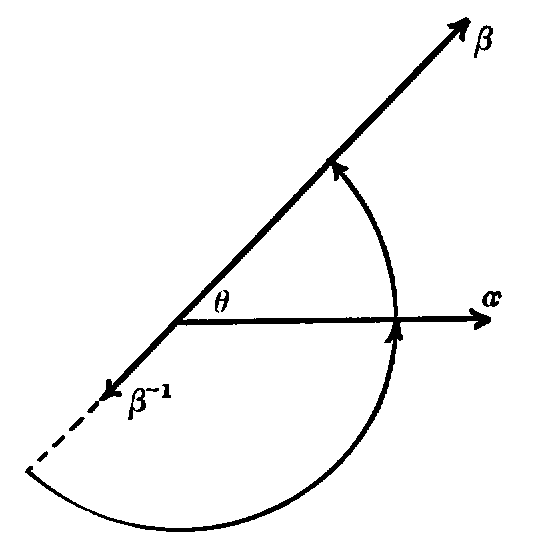
\includegraphics[width=80mm]{images/Image29.png}
\end{center}

For, since $\alpha\beta \cdot \beta^{-1} = \alpha$, therefore
$\alpha\beta$ turns through the angle from $\beta^{-1}$ to
$\alpha$, which is the supplement of the angle $\theta$ from
$\alpha$ to $\beta$.

\begin{itemize}
\item \textsc{Cor.} $S\alpha\beta = -T\alpha\beta\cos\theta$,
$TV\alpha\beta = T\alpha\beta\sin\theta$. [$Sq = Tq\cos\angle{q}$,
etc.]
\end{itemize}

\item \textit{The scalar of $\alpha\beta$ equals the product of
$\alpha$ and the projection of $\beta$ upon it; the vector of
$\alpha\beta$ equals the product of $\alpha$ and the projection of
$\beta$ perpendicular to it, and $V\alpha\beta$ is a vector
perpendicular to $\alpha$, $\beta$ on their counter-clockwise side
whose length equals the area of the parallelogram on $\alpha$,
$\beta$ as sides.}

\begin{center}
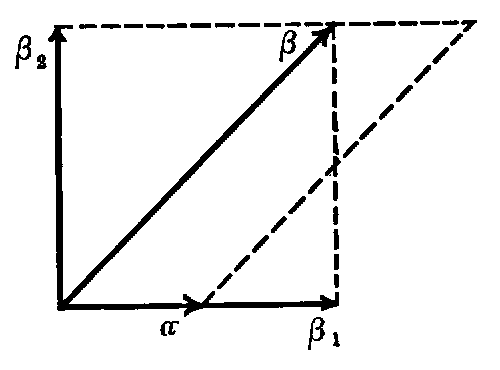
\includegraphics[width=80mm]{images/Image30.png}
\end{center}

Let $\beta_1$, $\beta_2$ be the components of $\beta$ parallel and
perpendicular to $\alpha$, then $\beta = \beta_1 + \beta_2$ and
$\alpha\beta = \alpha\beta_1 + \alpha\beta_2 =
\mathit{scalar+vector}$. Hence
\begin{equation*}
S\alpha\beta = \alpha\beta_1, \text{ as stated; and } V\alpha\beta =
\alpha\beta_2,
\end{equation*}
which is $\beta_2$ turned a counter-clockwise right angle round
$\alpha$ and lengthened by $T\alpha$. Hence $V\alpha\beta$ is
perpendicular to $\alpha$, $\beta$ on their counterclockwise side
(towards the reader in the figure), and its length is
$T\alpha \cdot T\beta_2 = $ area parallelogram on $\alpha$,
$\beta$, as sides.\footnote{The parallelogram on $\alpha$, $\beta$
may be considered as bounded by the path of a point that receives
the displacement $\alpha$, then the displacement $\beta$, then the
displacement $-\alpha$, then the displacement $-\beta$. This area
is therefore bounded \textit{counter-clockwise} round
$V\alpha\beta$ as axis; and $V\alpha\beta$ may therefore be called
the vector measure of the area of this directed parallelogram or
of any parallel plane area of the same magnitude and direction of
boundary.}

\begin{itemize}
\item \textsc{Cor.\ 1.} \textit{The projections of $\beta$
parallel and perpendicular to $\alpha$ equal
$\alpha^{-1}S\alpha\beta$ and $\alpha^{-1}V\alpha\beta$.}

\item \textsc{Cor.\ 2.} \textit{The scalar measure of the
projection of $\beta$ upon $\alpha$ is
$\frac{-S\alpha\beta}{T\alpha}$, and the tensor measure of the
projection of $\beta$ perpendicular to $\alpha$ is
$\frac{TV\alpha\beta}{T\alpha}$.} [Also from 58, Cor.]

\item \textsc{Cor.\ 3.} \textit{If $\theta$ be the angle between
$\alpha$, $\beta$, then $\cos\theta =
-\frac{S\alpha\beta}{T\alpha\beta}$, $\sin\theta =
\frac{TV\alpha\beta}{T\alpha\beta}$.} [Also from 58, Cor.]
\end{itemize}

\item \textit{The volume of a parallelepiped on $\alpha$, $\beta$,
$\gamma$ as edges is $-S\alpha\beta\gamma$ (the volume being
positive or negative according as $\alpha$ lies on the
counter-clockwise or clockwise side of $\beta$, $\gamma$).}

\begin{center}
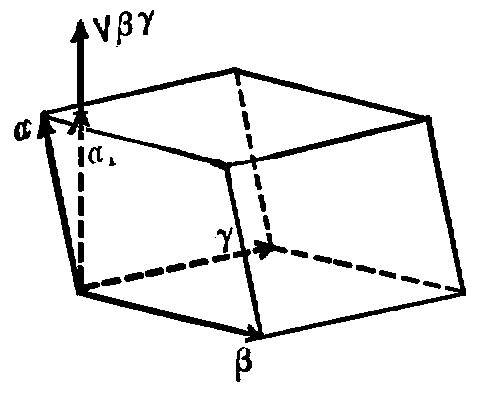
\includegraphics[width=80mm]{images/Image31.png}
\end{center}

For let $\alpha_1$ be the projection of $\alpha$ upon
$V\beta\gamma$; then taking the face $\beta$, $\gamma$ of the
parallelepiped as the base, we have by Art.\ 59 that
$TV\beta\gamma$ is the area of the base; also $T\alpha_1$ is the
altitude. Hence \textit{numerical volume}
\begin{align}
&= T\alpha_1 \cdot TV\beta\gamma = \mp\alpha_1 V\beta\gamma \tag*{[Art.\ 46.]}\\
&= \mp S\alpha{V}\beta\gamma = \mp{S}\alpha\beta\gamma. \tag*{[59,
56, \textit{d}.]}
\end{align}
The upper or lower sign must be taken according as $\alpha_1$,
$V\beta\gamma$ are in the same or opposite directions. This
numerical result must be multiplied by -1 when $\alpha$ lies on
the clockwise side of $\beta$, $\gamma$; i.e., when $\alpha_1$,
$V\beta\gamma$ are opposites (since $V\beta\gamma$ lies on the
counter-clockwise side of $\beta$, $\gamma$).
Hence---$S\alpha\beta\gamma$ is the required algebraic volume.

\begin{itemize}
\item \textsc{Cor.} \textit{The condition that $\alpha$, $\beta$,
$\gamma$ are coplanar vectors is that $S\alpha\beta\gamma = 0$ (or
$\alpha\beta\gamma =$ a vector)}.
\end{itemize}
\end{enumerate}

\addcontentsline{toc}{subsection}{Examples}
\subsection*{Examples}

\small \begin{enumerate}
\item Expand $(p+q+r)^2$, $(\alpha+\beta+\gamma)^2$, $(p+q)(p-q)$,
$(p-q)(p+q)$, $(p+q)K(p+q)$. Show that $T(p+q)^2 = Tp^2 + 2SpKq +
Tq^2$.

\item Solve $q^2+ 4\mathbf{k}q-8 = 0$ for $q$. [$q$ must be
cocircular with $\mathbf{k}$. Hence $q = -2\mathbf{k}\pm 2$ are
the real solutions.]

\item Find the tensor, versor, scalar, vector, and angle of each
of the numbers: $2$, $-3$, $3\mathbf{i}$, $2 + 3\mathbf{i}$,
$\mathbf{i+j}$, $3\mathbf{i}+4\mathbf{j}$,
$5e^{\frac{\pi}{3}\mathbf{i}}$,
$(2\mathbf{i}+3\mathbf{j}+6\mathbf{k})^2$.

\item Show that the three quaternion cube roots of $-1$, with
horizontal great circle, are $-1$,
$\frac{1}{2}\pm\frac{1}{2}\sqrt{3}\mathbf{k}$.

\item Show geometrically that
$e^{\theta\epsilon} + e^{-\theta\epsilon} = 2\cos\theta$,
$\epsilon^{\theta\epsilon} - e^{-\theta\epsilon} =
2\epsilon\sin\theta$.

\item The numbers $e^\alpha$ and
\begin{equation*}
1+\alpha+\frac{\alpha^2}{2!}+\frac{\alpha^3}{3!}+\frac{\alpha^4}{4!}+\cdots
\end{equation*}
are equal. Verify this approximately by geometric construction
when $T\alpha = 1$, and when $T\alpha = 2$. [For the series,
construct $\mathbf{OA}$, $\mathbf{AB} = \alpha\mathbf{OA}$,
$\mathbf{BC} = \frac{1}{2}\alpha\mathbf{AB}$, $\mathbf{CD} =
\frac{1}{3}\alpha\mathbf{BC}$, $\mathbf{DE} =
\frac{1}{4}\alpha\mathbf{CD}$, etc.]

\item In the plane triangle $ABC$, whose sides opposite $A$, $B$,
$C$, are $a$, $b$, $c$, show by squaring $\mathbf{BC = AC-AB}$,
that as $a^2 = b^2 + c^2 - 2bc\cos{A}$; also from
\begin{equation*}
V\mathbf{BCCA} = V\mathbf{CAAB} = V\mathbf{ABBC}
\end{equation*}
show that $a:b:c = \sin{A}:\sin{B}:\sin{C}$.

\item From $e^{\theta\epsilon} = \cos\theta + \epsilon\sin\theta$,
$e^{\theta\epsilon} \cdot e^{\theta'\epsilon} =
e^{(\theta+\theta')\epsilon}$, show that
\begin{align*}
\cos(\theta+\theta') &= \cos\theta\cos\theta' - \sin\theta\sin\theta', \\
\sin(\theta+\theta') &= \sin\theta\cos\theta' + \cos\theta\sin\theta'.
\end{align*}

\item Show that $(\cos\theta + \epsilon\sin\theta)^n =
\cos{n\theta} + \epsilon\sin{n\theta}$.

\item Show that $Spq = SpSq + S(Vp \cdot Vq)$, and hence that
$\cos\angle{pq} = \cos\angle{p} \cdot \cos\angle{q} + \sin\angle{p}
\cdot \sin\angle{q} \cdot \cos\angle{(Vp \cdot Vq)}$.

\item If $\text{arc } q = \overset\frown{BA}$, $\text{arc } p
= \overset\frown{AC}$, show that the last equation of Ex.\ 10 is
the property
\begin{equation*}
\cos{a} = \cos{b}\cos{c}+\sin{b}\sin{c}\cos{A}
\end{equation*}
of the spherical triangle $ABC$. [Draw $\overset\frown{B'A} =
\text{arc } Vq$, $\overset\frown{AC'} = \text{arc } Vp$.]

\item If $\alpha$, $\beta$, $\gamma$, $\alpha'$, $\beta'$,
$\gamma'$ are vectors from $O$ to the vertices $A$, $B$, $C$,
$A'$, $B'$, $C'$ of two spherical triangles on the unit sphere
$O$, where $\alpha' = UV\beta\gamma$, $\beta' = UV\gamma\alpha$,
$\gamma' = UV(\alpha\beta)$; then $\alpha = UV\beta'\gamma'$,
$\beta = UV\gamma'\alpha'$, $\gamma = UV\alpha'\beta'$, and the
two triangles are polar triangles.

\item In Ex.\ 12 show that $\cos\alpha = -S\beta\gamma$,
$\sin\alpha = TV\beta\gamma$, etc.; $\cos{A} = S(UV\gamma\alpha
\cdot UV\alpha\beta) = S\beta'\gamma' = -\cos\alpha'$, etc. Hence
$\angle{A}$, $\angle\alpha'$ are supplements, etc.

\item Show that the equation of Ex.\ 11 follows from the identity,
$-S\beta\gamma = S(\beta\gamma \cdot \gamma\alpha) = S\beta\gamma
\cdot S\gamma\alpha + S(V\gamma\alpha \cdot V\alpha\beta)$.

\item From $V(V\gamma\alpha \cdot V\alpha\beta) =
-\alpha{S}\alpha\beta\gamma$, and the similar equations found by
advancing the cyclic order $\alpha$, $\beta$, $\gamma$, show that
we have in the spherical triangle $ABC$,
\begin{equation*}
\sin{a}:\sin{b}:\sin{c} = \sin{A}:\sin{B}:\sin{C}.
\end{equation*}

\item Show that if $\alpha$, $\beta$, $\gamma$ are coplanar unit
vectors, then $\alpha\beta\gamma = -\alpha\beta^{-1} \cdot \gamma$
$=$ ($\gamma$ turned through the angle from $\beta$ to $\alpha$
and reversed) $=$ ($\beta$ rotated $180^{\circ}$ about the exterior
bisector of the angle between $\alpha$, $\gamma$) $=$
$(\alpha-\gamma)\beta(\alpha-\gamma)^{-1}$.

\item Show that $(V\mathbf{ABCD})^{-1}S\mathbf{AC}V\mathbf{ABCD}$
is the shortest vector from the line $AB$ to the line $CD$.
[Project $\mathbf{AC}$ upon the common perpendicular to $AB$,
$CD$.]

\item If $\alpha$, $\beta$, $\gamma$ be the vector edges about a
vertex of an equilateral pyramid (whose edges are unit lengths),
then $\beta-\gamma$, $\gamma-\alpha$, $\alpha-\beta$, are the
remaining vector edges. Hence show that $S\beta\gamma =
S\gamma\alpha = S\alpha\beta = -\frac{1}{2}$, and $V\alpha
V\beta\gamma = (-\beta)S\gamma\alpha + \gamma{S}\alpha\beta =
\frac{1}{2}(\beta-\gamma)$. Also show that:

\begin{enumerate}
\item The face angles are $60^{\circ}$, the area of a face is
$\frac{1}{4}\sqrt{3}$, and its altitude is $\frac{1}{2}\sqrt{3}$.

\item Opposite edges are perpendicular, and their shortest
distance is $\frac{1}{2}\sqrt{2}$.

\item The angle between a face and an edge is
$\cos^{-1}\frac{1}{3}\sqrt{3}$.

\item The angle between two adjacent faces is
$\sin^{-1}\frac{2}{3}\sqrt{2}$.

\item The volume and altitude of the pyramid are
$\frac{1}{12}\sqrt{2}$, $\frac{1}{3}\sqrt{3}$.
\end{enumerate}

\item The cosines of the angles that a vector makes with
$\mathbf{i}$, $\mathbf{j}$, $\mathbf{k}$, are called its
\textit{direction cosines}. Find the lengths and direction cosines
of
\begin{equation*}
\mathbf{2i-3j+6k}, \mathbf{i+2j-2k},
x\mathbf{i}+y\mathbf{j}+z\mathbf{k}.
\end{equation*}

\item Show that the sum of the squares of the direction cosines of
a line equals 1.

\item If $(l, m, n)$, $(l', m', n')$ are the direction cosines of
two lines, show that $l\mathbf{i}+m\mathbf{j}+n\mathbf{k}$,
$l'\mathbf{i}+m'\mathbf{j}+n'\mathbf{k}$, are unit vectors in the
directions of the lines, and that if $\theta$ be the angle between
the lines, then $\cos\theta = ll'+mm'+nn'$; also that $\sin^2
\theta =
\begin{vmatrix}
m & n   \\
m' & n' \\
\end{vmatrix}^2
+
\begin{vmatrix}
n & l   \\
n' & l' \\
\end{vmatrix}^2
+
\begin{vmatrix}
l & m   \\
l' & m' \\
\end{vmatrix}^2$,
and that the three terms of the second member, respectively
divided by $\sin^2\theta$, are the squares of the direction
cosines of a line that is perpendicular to the given lines. [Art.\
57.]

\item If $O$ be a given origin, then the vector $\mathbf{OP} =
\rho = x\mathbf{i} + y\mathbf{j} + z\mathbf{k}$ say, is called the
\textit{vector of $P$ with reference to the given origin}. If
$OX$, $OY$, $OZ$ be axes in the directions of $\mathbf{i}$,
$\mathbf{j}$, $\mathbf{k}$, the scalar values of the projections
of $\mathbf{OP}$ upon these axes, \textit{i.e.}, $(x,y,z)$, are
called the \textit{co\"{o}rdinates of $P$ with reference to the given
axes}. Let the co\"{o}rdinates of the vertices of the pyramid $ABCD$
be, respectively, (8,2,7), (10,6,3), (1,6,3), (9,10,11). Draw
this pyramid with reference to a perspective of $\mathbf{i}$,
$\mathbf{j}$, $\mathbf{k}$, showing co\"{o}rdinates and vectors. Also:

\begin{enumerate}
\item Find the vectors and co\"{o}rdinates of the middle points of the
edges. \linebreak[4] [$\mathbf{OM} = \frac{1}{2}\mathbf{(OA + OB)}$, etc.]

\item Find the lengths and direction cosines of the edges.
[$\mathbf{-AB^2} = AB^2$, etc.]

\item Find vectors that bisect the face angles. [$U\mathbf{AC}
{\pm}U\mathbf{AD}$ bisects $\angle CAD$.]

\item Find altitudes of the faces and the vectors of their feet.
[If $L$ be the foot of the perpendicular from $B$ on $AC$, then
$\mathbf{AL = AB^{-1}}S\mathbf{ABAC}$, etc.]

\item Find the areas of the faces.

\item Find the volume and altitudes of the pyramid.

\item Find the angles between opposite edges, and their (shortest)
distance apart. [Ex.\ 17.]

\item Find the angle between two adjacent faces.
\end{enumerate}
\end{enumerate} \normalsize

\newpage
\chapter{Equations of First Degree}

\addcontentsline{toc}{section}{Scalar Equations, Plane and
Straight Line}

\begin{enumerate}
\setcounter{enumi}{60}

\item The general equation of first degree in an unknown vector
$\rho$ is of the form,

\begin{enumerate}
\item $q_1{\rho}r_1+q_2{\rho}r_2+\cdots = q$,
\end{enumerate}

where $q$, $q_1$, $r_1$, $q_2$, $r_2$, $\cdots$ are known numbers.

This equation may be resolved into two equations by taking the
scalar and the vector of each member; and we shall consider these
equations separately.

\item Taking the scalar of (\textit{a}), Art.\ 61, the term
$Sq_1{\rho}r_1$ becomes, by a cyclic change in the factors,
$S \cdot r_1q_1\rho$, and this becomes [by dropping the vector
$(Sr_1q_1)\rho$, since its scalar is zero] $S(Vr_1q_1 \cdot \rho)$;
and similarly for the other terms. Hence if we put
$Vr_1q_1 + Vr_2q_2 + \cdots = \delta$, and $Sq = d$, the general
scalar equation of first degree in $\rho$ becomes,

\begin{enumerate}
\item $S\delta\rho = d$ or $S\delta(\rho - d\delta^{-1}) = 0$.
\end{enumerate}

One solution of this equation is obviously $\rho = d\delta^{-1}$.
This is not the only solution, since by Art.\ 45, Cor.\ 3, the
second factor may be any vector that is perpendicular to $\delta$.
Hence the general solution is $\rho = d\delta^{-1} + V\sigma\delta$,
where $\sigma$ is an arbitrary vector.

\item Hence, draw $\mathbf{OD} = \delta$, take $N$ on the line
$OD$ so that $\mathbf{ON} = d\delta^{-1}$, and draw any vector
$\mathbf{NP} = V\sigma\delta$ that is perpendicular to the line
$OD$; then $\rho = \mathbf{OP}$ is a solution of the equation
$S\delta\rho = d$.

\begin{center}
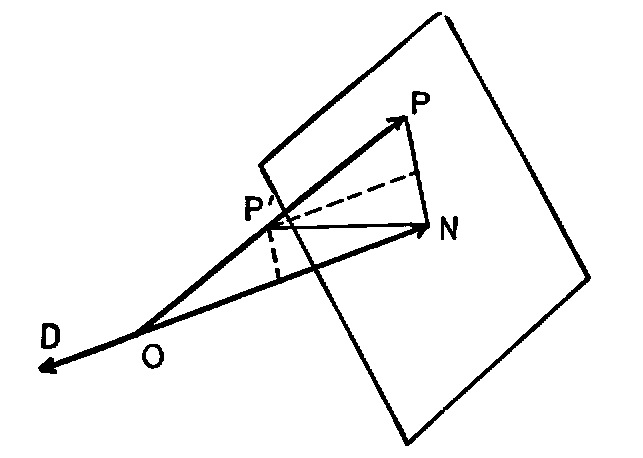
\includegraphics[width=80mm]{images/Image32.png}
\end{center}

The locus of $P$ is therefore a plane perpendicular to $OD$ at the
point $N$; and this plane is called \textit{the locus of the
equation $S\delta\rho = d$, with respect to the origin O}. [The
locus is the assemblage of all points that satisfy the equation.]

\item \textit{The vector perpendicular distance from the plane
$S\delta\rho - d = 0$ to the point $P'$ (whose vector is $\rho'$) is
$\delta^{-1}(S\delta\rho' - d)$, and the corresponding scalar
distance measured upon $\delta$ is}
\begin{equation*}
\frac{-(S\delta\rho'-d)}{T\delta}.
\end{equation*}

For the perpendicular distance of $P'$ is the projection of
$\mathbf{NP'} = (\rho' - d\delta^{-1})$, upon $\mathbf{OD} =
\delta$.

\item \textit{The locus of the simultaneous equations $Sa\rho =
a$, $S\beta\rho = b$ is a straight line, viz., the intersection of
the two plane loci of these equations taken separately.}

For in order that $\rho = \mathbf{OP}$ may satisfy both equations,
$P$ must lie in both planes, and its locus is therefore the
intersection, of those planes.

\item The equation $V\delta\rho = \delta'$, or
\begin{equation*}
V\delta(\rho - \delta^{-1}\delta') = 0,
\end{equation*}
is a consistent equation only when $\delta'$ is perpendicular to
$\delta$, since $V\delta\rho$ is always perpendicular to $\delta$.
When $\delta'$ is perpendicular to $\delta$, then
$\delta^{-1}\delta'$ is a vector (Art.\ 45, Cor.\ 1), and the
general solution of this equation is $\rho =
\delta^{-1}\delta' + x\delta$, where $x$ is an arbitrary scalar
(Art.\ 46, Cor.). Hence draw $\mathbf{ON} = \delta^{-1}\delta'$,
and $\mathbf{NP} = x\delta$ (any vector parallel to $\delta$), and
then $\rho = \mathbf{OP}$ is a solution of the given equation. The
locus of $P$ is therefore the straight line through $N$ parallel
to $\delta$, and $\mathbf{ON}$ is the perpendicular from the
origin upon the line. The equations of Art.\ 65 take this form by
multiplying the first by $\beta$, the second by $\alpha$, and
subtracting, remembering that
\begin{equation*}
V(V\alpha\beta \cdot \rho) = \alpha{S}\beta\rho - \beta{S}\alpha\rho.
\end{equation*}

\begin{center}
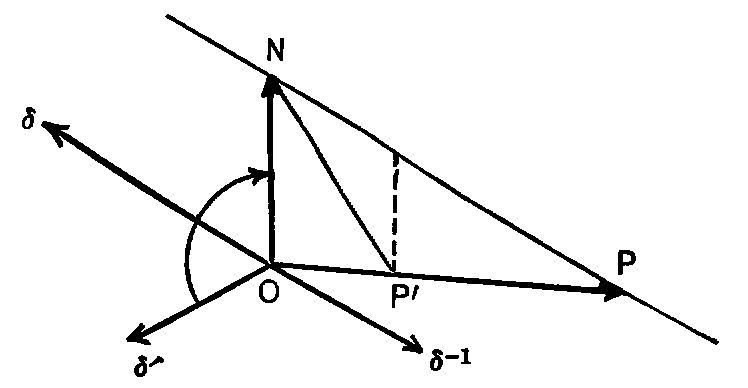
\includegraphics[width=80mm]{images/Image33.png}
\end{center}

\item \textit{The vector perpendicular distance from the line
$V\delta\rho-\delta' = 0$ to the point $\mathbf{P'}$ is
$\delta^{-1}(V\delta\rho'-\delta')$, where $\rho' =
\mathbf{OP'}$.}

For the required perpendicular distance of $P'$ is the projection
of $\mathbf{NP'}$, $=(\rho' - \delta^{-1}\delta')$, perpendicular
to $\delta$.

\item \textit{The point of intersection of the three planes}
$S\alpha\rho = a$, $S\beta\rho = b$, $S\gamma\rho = c$ \textit{is}
\begin{equation}
\rho = \frac{(aV\beta\gamma + bV\gamma\alpha +
cV\alpha\beta)}{S\alpha\beta\gamma}. \tag*{[Art. 56, (\textit{j}).]}
\end{equation}
\end{enumerate}

\addcontentsline{toc}{subsection}{Examples}
\subsection*{Examples}

\small \begin{enumerate}
\item Find the equation of the locus of a point that moves
so that its numerical distances from two fixed points are equal.

\item A point moves so that its scalar distances from two fixed
planes are equal; show that its locus is a plane bisector of the
diedral angle of the given planes.

\item A point moves so that the sum or difference of its scalar
distances from two fixed planes is constant; show that its locus
is a plane parallel to the interior or exterior bisector of the
diedral angle of the given planes.

\item A point moves so that the ratio of its scalar distances from
two fixed planes is constant; show that its locus is a plane.

\item A point moves so that its numerical distances from two
intersecting lines are equal; find its locus. [Take the point of
intersection as origin.]

\item A point moves so that its numerical distances from three
fixed points are equal; find its locus.

\begin{enumerate}
\item The same with coplanar lines instead of points. [Four
straight lines perpendicular to the plane of the lines.]
\end{enumerate}

\item Find the vector of the centre of the sphere whose surface
passes through four given points.

\item A point moves so that its tangential distances from two
given spheres are numerically equal; find its locus.

\item On the chord $\mathbf{OQ}$ of a given sphere a point $P$ is
taken so that $\mathbf{OP \cdot OQ} = -a^2$; when $Q$ moves round
the sphere find the locus of $P$. [A plane perpendicular to the
diameter $OD$.]

\item The locus of the point $P$ whose co\"{o}rdinates $(x, y, z)$
satisfy $lx + my + nz + d = 0$ is a plane perpendicular to the
vector $l\mathbf{i} + m\mathbf{j} + n\mathbf{k}$, at a distance
from the origin of $-d/\sqrt{l^2 + m^2 + n^2}$, measured in the
direction of this vector. (\textit{a}) Show that the equation of
this plane may be put in the form $x\cos\alpha + y\cos\beta +
z\cos\gamma - p = 0$, where $p$ is the perpendicular distance from
$O$ to the plane and the cosines are the direction cosines of this
perpendicular.

\item Find the perpendicular distance of $P' = (x', y', z')$, from
the plane of Ex.\ 10,
\begin{equation*}
[x'\cos\alpha + y'\cos\beta + z'\cos\gamma - p].
\end{equation*}

\item The locus of the point $P$ whose co\"{o}rdinates $(x, y, z)$
satisfy $\frac{(x - a)}{l} = \frac{(y - b)}{m} = \frac{(z -
c)}{n}$ is a line parallel to the vector $l\mathbf{i} +
m\mathbf{j} + n\mathbf{k}$ through the point $(a, b, c)$. If $P$
satisfy the first two of these three equations, its locus is a
plane through the line, perpendicular to the plane of $XOY$. [If
$t$ be the common value of the three ratios, then $\rho =
a\mathbf{i} + b\mathbf{j} + c\mathbf{k} + t(l\mathbf{i} +
m\mathbf{j} + n\mathbf{k})$.]

\item Find the perpendicular distance of $P' = (x', y', z')$ from
the line of Ex.\ 12.

\smallskip
In the following examples $A$, $B$, $C$, $D$, $P$ are points whose
co\"{o}rdinates are $(8, 2, 7)$, $(10, 6, 3)$, $(1, 6, 3)$, $(9,
10,11)$, $(x, y, z)$.

\smallskip
\item The equation of the plane through $A$ perpendicular to $OD$
is $S\mathbf{ODAP} = 0$, or $9x + 10y + 11z = 169$.

\item The equation of the plane through $AB$ parallel to $CD$ is
$S \cdot \mathbf{AP}V\mathbf{ABCD} = 0$, or $2x - 2y - z = 5$.

\item The equation of the plane $ABC$ is $S \cdot
\mathbf{AP}V\mathbf{ABAC} = 0$ or $y + z = 9$.

\item Find the perpendicular distance of $D$ from the planes in
Exs.\ 14, 15, 16.

\item The equation of the plane through $AB$ that contains the
common perpendicular to $AB$, $CD$ is
\begin{equation*}
S \cdot \mathbf{AP}V(\mathbf{AB}V\mathbf{ABCD}) = 0, \text{ or }
2x + y + 2z = 32.
\end{equation*}

\item The equation of the line through $A$ parallel to $OD$ is
$V\mathbf{ODAP} = 0$ or $\mathbf{AP} = t\mathbf{OD}$, or $\frac{(x -
8)}{9} = \frac{(y - 2)}{10} = \frac{(z - 7)}{11}$.

\item The equation of the line $AB$ is $V\mathbf{ABAP} = 0$, or
$\mathbf{AP} = t\mathbf{AB}$ or $\frac{(x - 8)}{2} = \frac{(y -
2)}{4} = \frac{(z - 7)}{-4}$.

\item The equation of the common perpendicular to $AB$, $CD$ is
the equation of Ex.\ 18 and $x + 2y - 2z = 7$.

\item Find the distance of $D$ from the lines in Exs.\ 19, 20, 21.

\item Find $\mathbf{OD}$ in the form $l\mathbf{OA} + m\mathbf{OB}
+ n\mathbf{OC}$, and find the ratios in which $OD$ cuts the
triangle $ABC$.
\end{enumerate} \normalsize

\addcontentsline{toc}{section}{\textbf{Nonions}}
\section*{Nonions}

\addcontentsline{toc}{section}{Vector Equations, the Operator
$\phi$}

\begin{enumerate}
\setcounter{enumi}{68}

\item The vector equation of first degree is
\begin{equation}
Vq_1\rho r_1 + Vq_2\rho r_2 + \cdots = Vq. \tag*{(\textit{a})}
\end{equation}

To solve this equation we resolve it along $\mathbf{i, j, k}$, by
multiplying it by these vectors and taking the scalars of the
products. We thus find three scalar equations of first degree from
which $\rho$ may be immediately found as in Art.\ 68. Hence
(\textit{a}) has in general one, and only one, solution which
corresponds to the intersection of three given planes. [See
further Art.\ 81.]

\item The first member of Art.\ 69 (\textit{a}) is a
\textit{linear, homogeneous vector function of} $\rho$;
\textit{i.e.}, it is of first degree in $\rho$, every term is of
the same degree in $\rho$, and it is a vector.

We may denote the operator
\begin{equation*}
Vq_1()r_1 + Vq_2()r_2 + \cdots
\end{equation*}
by a single letter, $\phi$, so that $\phi\rho, \phi\sigma, \cdots$
denote the vectors that result from putting $\rho, \sigma, \cdots$
in the places occupied by the parenthesis.

\item \textit{The operator} $\phi$ \textit{is distributive over a
sum and commutative with scalars; i.e.},
\begin{equation*}
\phi(x\rho + y\sigma) = x\phi\rho + y\phi\sigma.
\end{equation*}

This is immediately verified by putting $x\rho + y\sigma$ in the
places occupied by the parentheses of $\phi$ and expanding the
several terms.

\item We have $\rho = x\alpha + y\beta + z\gamma$, where $\alpha,
\beta, \gamma$ are given non-coplanar vectors, and $x, y, z$, are
scalars, each of first degree in $\rho$, as shown in
56(\textit{i}) with $\rho$ in the place of $\delta$; hence,
\begin{equation}
\phi\rho = x\phi\alpha + y\phi\beta + z\phi\gamma. \tag*{(\textit{a})}
\end{equation}

The complete operation of $\phi$ is therefore determined when the
three vectors $\phi\alpha, \phi\beta, \phi\gamma$ are known. Since
each of these vectors involves three scalar constants
(\textit{e.g.}, the multiples of the given non-coplanar vectors
$\alpha$, $\beta$, $\gamma$, that express it), therefore the value
of $\phi$ depends upon nine scalar constants. The operator $\phi$
may therefore be called a \textit{nonion}. Scalars and rotators
are particular forms of nonions.

\small \textsc{Note.}---It is readily shown that nonions have the
same laws of addition and multiplication among themselves as
quaternions. Products are not in general commutative. A product
\begin{equation*}
(\phi - g_1) (\phi - g_2) (\phi - g_3),
\end{equation*}
where $g_1$, $g_2$, $g_3$ are scalars, is commutative, since
$\phi$ is commutative with scalars by Art.\ 71. Hence this product
multiplies out as if $\phi$ were a scalar, and is
\begin{equation*}
\phi^3 - (g_1 + g_2 + g_3)\phi^2 + (g_2 g_3 + g_3 g_1 + g_1
g_2)\phi - g_1 g_2 g_3.
\end{equation*} \normalsize

\addcontentsline{toc}{section}{Linear Homogeneous Strain}
\section*{Linear Homogeneous Strain}

\item An elastic solid is \textit{subjected to the strain $\phi$
with respect to an origin $O$}, when all its particles, $A$, $B$,
$C$, etc., are displaced to positions $A'$, $B'$, $C'$, etc., that
are determined by $\mathbf{OA'} = \phi \mathbf{OA}$, $\mathbf{OB'}
= \phi \mathbf{OB}$, $\mathbf{OC'} = \phi \mathbf{OC}$, etc. In
general, any particle $P$ whose vector is $\mathbf{OP} = \rho$
occupies after the strain the position $P'$, whose vector is
$\mathbf{OP'} = \phi\rho$. The particle at $O$ is not moved, since
its vector after strain is $\phi\mathbf{OO} = \phi 0 = 0$.

\begin{center}
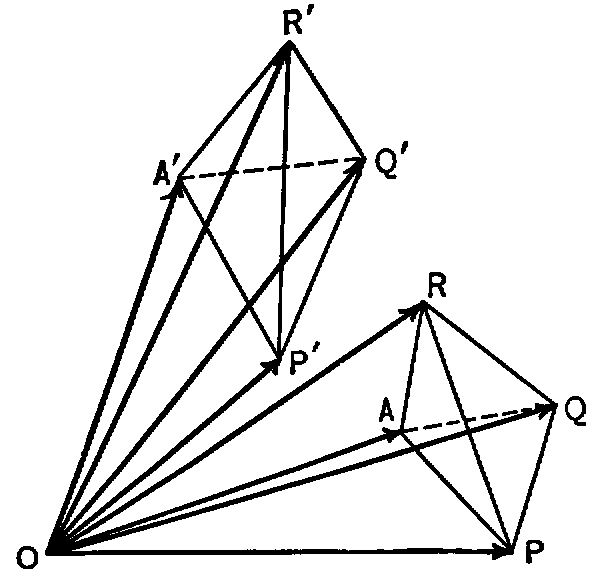
\includegraphics[width=80mm]{images/Image34.png}
\end{center}

\begin{enumerate}
\item We have, also, $\phi\mathbf{AP} = \mathbf{A'P'}$, etc.
\end{enumerate}

For,
\begin{align*}
\mathbf{A'P'} &= \mathbf{OP'} - \mathbf{OA'} = \phi\mathbf{OP} - \phi\mathbf{OA} \\
              &= \phi(\mathbf{OP} - \mathbf{OA}) = \phi\mathbf{AP}, \text{ etc.}
\end{align*}

\item \textit{A straight line of particles parallel to $\alpha$ is
homogeneously stretched and turned by the strain $\phi$ into a
straight line of particles parallel to $\phi\alpha$, and the ratio
of extension and turning is $\phi\alpha / \alpha$.}

For let $AP$ be a line parallel to $\alpha$, and let $A$, $P$
strain into $A'$, $P'$. Then, since $\mathbf{AP} = x\alpha$,
therefore, by 73\textit{a}, $\mathbf{A'P'} = x\phi\alpha$, and the
ratio of extension and turning is $\mathbf{A'P'/AP} = \phi
\alpha/\alpha$.

\small \textsc{Note.}---This property that parallel lengths of
the substance strain into parallel lengths and are stretched
proportionally, is the physical definition of \textit{linear
homogeneous strain}. \normalsize

\item \textit{A plane of particles parallel to $\alpha$, $\beta$
is homogeneously spread and turned by the strain $\phi$ into a
plane of particles parallel to $\phi\alpha$, $\phi\beta$, and the
ratio of extension and turning is
$V\phi\alpha\phi\beta / V\alpha\beta$.}

For let $APQ$ be a plane parallel to $\alpha$, $\beta$, and let
$A$, $P$, $Q$ strain into $A'$, $P'$, $Q'$. Then, since
$\mathbf{AP} = x\alpha + y\beta$, $\mathbf{AQ} = x'\alpha +
y'\beta$, therefore
\begin{equation*}
\mathbf{A'P'} = x\phi\alpha + y\phi\beta, \quad
\mathbf{A'Q'} = x'\phi\alpha + y'\phi\beta.
\end{equation*}

By Arts.\ 59, 55, (\textit{e}), the directed area of the triangle
$APQ$ is $\frac{1}{2} V \cdot \mathbf{AP} \cdot \mathbf{AQ} =
\frac{1}{2}(xy' - x'y)V\alpha\beta$, and the directed area of the
triangle $A'P'Q'$ is the same multiple of $V\phi\alpha\phi\beta$.
Hence the ratio of the extension and turning of directed area is
$V\phi\alpha\phi\beta / V\alpha\beta$.

\item \textit{A volume of particles is homogeneously dilated by
the strain $\phi$ in the ratio
\begin{equation*}
S\phi\alpha\phi\beta\phi\gamma / S\alpha\beta\gamma,
\end{equation*}
where $\alpha$, $\beta$, $\gamma$ are any given non-coplanar
vectors.}

For let the pyramid $APQR$ strain into the pyramid $A'P'Q'R'$.
Then since
\begin{equation*}
\mathbf{AP} = x\alpha + y\beta + z\gamma, \quad
\mathbf{AQ} = x'\alpha + y'\beta + z'\gamma,
\end{equation*}
$\mathbf{AR} = x''\alpha + y''\beta + z''\gamma$, therefore
$\mathbf{A'P'}$, $\mathbf{A'Q'}$, $\mathbf{A'R'}$ have these
values with $\phi\alpha$, $\phi\beta$, $\phi\gamma$ instead of
$\alpha$, $\beta$, $\gamma$. The volume of the pyramid $APQR$
relative to the order $AP$, $AQ$, $AR$ of its edges is, by Arts.\
60, 56, (\textit{c}),
\begin{equation*}
-\frac{1}{6}S\mathbf{APAQAR} =
-\frac{1}{6}\left|\begin{array}{lll}
                            x   & y   & z   \\
                            x'  & y'  & z'  \\
                            x'' & y'' & z'' \end{array} \right|
  S\alpha\beta\gamma,
\end{equation*}
while that of the strained pyramid is the same multiple of
$S\phi\alpha\phi\beta\phi\gamma$. Hence the ratio of dilation of
volume is $S\phi\alpha\phi\beta\phi\gamma / S\alpha\beta\gamma$.

\item The ratio of dilation of $\phi$ is called its
\textit{modulus}.

\begin{enumerate}
\item It is obvious from the signification of the modulus that
\textit{the modulus of a product of nonions equals the product of
the moduli of the factors; e.g.}, $\textit{mod } \phi\psi =
\textit{mod } \phi \cdot \textit{mod } \psi$.
\end{enumerate}

When $\text{mod }\phi$ is positive, the parts of the volume are
in the same order before and after strain. When $\text{mod }\phi$
is negative, the order of the parts is reversed by the strain;
\textit{i.e.}, if $AP$ lie on the counter-clockwise side of the
plane $AQR$, then $A'P'$ lies on the clockwise side of $A'Q'R'$,
so that the particles along $AP$ have been strained through the
particles of the plane $AQR$. Such a strain is obviously not a
physical possibility.

\addcontentsline{toc}{section}{Finite and Null Strains}
\section*{Finite and Null Strains}

\item \textit{If an elastic solid which fills all space be
subjected to a strain $\phi$, the strained solid fills all space
if $\text{mod }\phi$ be finite, and it fills only an indefinite
plane or line through the origin or reduces to the origin if
$\text{mod }\phi$ be zero.}

For if $S\phi\alpha\phi\beta\phi\gamma$ be finite, then
$\phi\alpha$, $\phi\beta$, $\phi\gamma$ are non-coplanar vectors,
so that
\begin{equation*}
\phi\rho( = x\phi\alpha + y\phi\beta + z\phi\gamma)
\end{equation*}
may be made any vector by properly choosing
$\rho(= x\alpha + y\beta + z\gamma)$. But if
$S\phi\alpha\phi\beta\phi\gamma = 0$, then $\phi\alpha$,
$\phi\beta$, $\phi\gamma$ are coplanar vectors or colinear vectors
or each zero, so that $\phi\rho$ will be a vector in a given plane
or line through $O$ or the vector of $O$, whatever value be given
to $\rho$.

When $\text{mod }\phi$ is zero, $\phi$ is called a \textit{null}
nonion; and it is called \textit{singly} or \textit{doubly} or
\textit{triply} null, according as it strains a solid into a
\textit{plane} or a \textit{line} or a \textit{point}. If
$\phi\alpha = 0$, then $\alpha$ is called a \textit{null
direction} of $\phi$.

\item \textit{Null strains, and only null strains, can have null
directions; a singly null strain has only one null direction; a
doubly null strain has a plane of null directions only; a triply
null strain has all directions null.}

For when $\text{mod }\phi = 0$, then $\phi\alpha$, $\phi\beta$,
$\phi\gamma$ are coplanar or colinear vectors, and we have a
relation $l\phi\alpha + m\phi\beta + n\phi\gamma = 0$, \textit{i.e.},
$l\alpha + m\beta + n\gamma$ is a null direction of $\phi$.
Conversely, if $\phi$ have a null direction, take one of the three
non-coplanar vectors $\alpha$, $\beta$, $\gamma$, in that
direction, say $\alpha$, and we have
$S\phi\alpha\phi\beta\phi\gamma = 0$, since $\phi\alpha = 0$, and
therefore $\mathrm{mod}\phi = 0$.

Also, if $\phi$ have only one null direction, $\alpha$, then
$\phi\beta$, $\phi\gamma$, are not parallel, since $\phi\beta =
l\phi\gamma$ makes $\beta - l\gamma$ a second null direction. Since
$\rho = x\alpha + y\beta + z\gamma$, therefore $\phi\rho =
y\phi\beta + z\phi\gamma$, which is any vector in the plane through
$O$ parallel to $\phi\beta$, $\phi\gamma$; hence $\phi$ is singly
null.

But if $\phi$ have two null directions, $\alpha$, $\beta$, then
$\phi\rho = z\phi\gamma$, which is any vector in the line through
$O$ parallel to $\phi\gamma$, and therefore $\phi$ is doubly null.
Also, since $\phi(x\alpha + y\beta) = 0$, therefore any direction in
the plane of $\alpha$, $\beta$ is a null direction of $\phi$.

If $\phi$ have three non-coplanar null directions $\alpha$,
$\beta$, $\gamma$, then $\phi\rho = 0$ for all values of $\rho$;
\textit{i.e.}, a \textit{triply} null nonion is identically zero.

\item \textit{A singly null nonion strains each line in its null
direction into a definite point of its plane; and a doubly null
nonion strains each plane that is parallel to its null plane into
a definite point of its line.}

For when $\phi$ is singly null, say $\phi\alpha = 0$, then
$x\phi\beta + y\phi\gamma$ is the vector of any point in the plane
of $\phi$, and all particles that strain into this point have the
vectors $\rho = x\alpha + y\beta + z\gamma$, where $x$ is
arbitrary, since $\phi\alpha = 0$; \textit{i.e.}, they are
particles of a line parallel to $\alpha$. So, if $\phi$ is doubly
null, say $\phi\alpha = 0$, $\phi\beta = 0$, then any point of the
line of $\phi$ is $z\phi\gamma$, and the particles that strain
into this point have the vectors
\begin{equation*}
\rho = x\alpha + y\beta + z\gamma,
\end{equation*}
in which $x$, $y$ are arbitrary; \textit{i.e.}, they are particles
of a plane parallel to $\alpha$, $\beta$.

\small \textsc{Note.}---It follows similarly that the strain
$\phi$ alters the dimensions of a line, plane, or volume by as
many dimensions as the substance strained contains independent
null directions of $\phi$, and no more. Hence, a product
$\phi\psi$ has the null directions of the first factor, and the
null directions of the second factor that lie in the figure into
which the first factor strains, and so on; the order of nullity of
a product cannot exceed the sum of the orders of its factors, and
may be less; etc. \normalsize

\addcontentsline{toc}{section}{Solution of $\phi\rho = \delta$}
\section*{Solution of $\phi\rho = \delta$}

\item The solutions of $\phi\rho = \delta$ are, by definition of
the strain $\phi$, the vectors of the particles that strain into
the position whose vector is $\delta$. Hence:

\begin{enumerate}
\item When $\phi$ is finite, there is one, and only one, solution.

\item When $\phi$ is singly null, and $\delta$ does not lie in the
plane of $\phi$, there is no finite solution. Divide the equation
by $T\rho$, and make $T\rho$ infinite, and we find $\phi U \rho =
0$; \textit{i.e.}, the vector of the point at infinity in the null
direction of $\phi$ is a solution.

\item When $\phi$ is singly null, and $\delta$ lies in the plane
of $\phi$, there are an infinite number of solutions,
\textit{viz.}, the vectors of the particles of a line that is
parallel to the null direction of $\phi$.

\item When $\phi$ is doubly null, and $\delta$ does not lie in the
line of $\phi$, there is no finite solution. As in (2) the vectors
of the points of the line at infinity in the null plane of $\phi$
are solutions.

\item When $\phi$ is doubly null, and $\delta$ lies in the line of
$\phi$, there are an infinite number of solutions, \textit{viz.},
the vectors of the particles of a plane that is parallel to the
null plane of $\phi$.
\end{enumerate}

These results correspond to the intersections of three planes,
viz.:
\begin{enumerate}
\item The three planes meet in a point.
\item The three planes parallel to a line.
\item The three planes meet in a common line.
\item The three planes parallel.
\item The three planes coincide.
\end{enumerate}

\addcontentsline{toc}{section}{Derived Moduli. Latent Roots}
\section*{Derived Moduli of $\phi$}

\item The ratio in which the nonion $\phi+g$ dilates volume is,
\begin{equation*}
\text{mod }(\phi+g) = S(\phi\alpha + g\alpha)(\phi\beta +
g\beta)(\phi\gamma + g\gamma) / S\alpha\beta\gamma.
\end{equation*}
This is independent of the values of the non-coplanar vectors
$\alpha$, $\beta$, $\gamma$ in terms of which it is expressed. If
$g$ is a scalar, this modulus is an ordinary cubic in $g$, whose
coefficients will therefore depend only upon $\phi$. The constant
term is $\text{mod }\phi$, and the coefficients of $g$, $g^2$,
are called $\text{mod}_1 \phi$, $\text{mod}_2 \phi$, so that,
\begin{equation}
\text{mod }(\phi + g) = g^3 + g^2 \text{mod}_2 \phi
+ g \text{mod}_1 \phi + \text{mod } \phi. \tag*{(\textit{a})}
\end{equation}
\begin{align*}
[\mathrm{mod}_1 \phi &= S(\alpha\phi\beta\phi\gamma
     + \beta\phi\gamma\phi\alpha + \gamma\phi\alpha\phi\beta)
   / S\alpha\beta\gamma; \\
\mathrm{mod}_2 \phi &= S(\beta\gamma\phi\alpha
     + \gamma\alpha\phi\beta + \alpha\beta\phi\gamma)
   / S\alpha\beta\gamma].
\end{align*}

\item The roots $g_1$, $g_2$, $g_3$, of the cubic
\begin{equation*}
\text{mod }(\phi-g) = 0
\end{equation*}
are called \textit{the latent roots of} $\phi$. We have from
82 (\textit{a}) with $-g$ in the place of $g$, and the
theory of equations,
\begin{gather*}
\text{mod }\phi = g_1 g_2 g_3, \quad
\text{mod}_1 \phi = g_2 g_3 + g_3 g_1 + g_1 g_2, \\
\text{mod}_2 \phi = g_1 + g_2 + g_3.
\end{gather*}

\begin{enumerate}
\item \textit{The latent roots of $\phi-g_1$ are those of $\phi$
diminished by $g_1$.}

For the roots of $\text{mod }(\phi - g_1 - g) = 0$, are $g=0$,
$g_2 - g_1$, $g_3 - g_1$. \textit{E.g.}, $g = g_2 - g_1$ gives
\begin{equation*}
\text{mod }[\phi - g_1 -(g_2 - g_1)] = \text{mod }(\phi - g_2) = 0.
\end{equation*}

\item \textit{The order of nullity of $\phi$ cannot exceed the
number of its zero latent roots.}

For if $\phi$ has one null direction $\alpha$, then $\phi\alpha =
0$ makes $\text{mod }\phi = 0$, so that at least one of the
latent roots is zero, say $g_1$; and if $\phi$ has a second null
direction $\beta$, then $\phi\alpha = 0$, $\phi\beta = 0$, makes
$\mathrm{mod}_1\phi = 0$ or $g_2g_3 = 0$, so that another latent
root is zero, etc.

\item \textit{The order of nullity of $\phi - g_1$ cannot exceed
the number of latent roots of $\phi$ that equal $g_1$.}
[(\textit{a}), (\textit{b})]
\end{enumerate}

\addcontentsline{toc}{section}{Latent Lines and Planes}
\section*{Latent Lines and Planes of $\phi$}

\item Those lines and planes that remain unaltered in geometrical
position by the strain $\phi$ are called \textit{latent lines and
planes of $\phi$}.

\begin{enumerate}
\item \textit{The latent directions of $\phi$ are the null
directions of $\phi - g_1$, $\phi - g_2$, $\phi - g_3$, and $g_1$,
$g_2$, $g_3$ are the corresponding ratios of extension in those
directions.}
\end{enumerate}

For if $\rho$ is any latent direction, and $g$ is the ratio of
extension in that direction, then we have $\phi\rho = g\rho$ or
$(\phi - g)\rho = 0$. Hence $\phi - g$ is a null nonion, or
$\text{mod }(\phi - g) = 0$, so that $g$ is a latent root of
$\phi$; also $\rho$ is a null direction of $\phi - g$.

\small \textsc{Note.}---Since a cubic with real coefficients has
at least one real root, therefore a real nonion has at least one
latent direction. Also if two roots are imaginary, they are
conjugate imaginaries, and the corresponding latent directions
must also be conjugate imaginaries. \normalsize

\item \textit{If $\alpha$, $\beta$, $\gamma$ be the latent
directions corresponding to $g_1$, $g_2$, $g_3$, then $(\beta,
\gamma)$, $(\gamma, \alpha)$, $(\alpha, \beta)$ determine latent
planes of $\phi$ in which the ratios of spreading are $g_2 g_3$,
$g_3 g_1$, $g_1 g_2$. E.g.,}
\begin{equation*}
V \phi \beta \phi \gamma = V (g_2 \beta \cdot g_3 \gamma) = g_2
g_3 V \beta \gamma .
\end{equation*}

Hence, in the general case when the latent roots are all unequal,
the latent vectors $\alpha$, $\beta$, $\gamma$ must form a
non-coplanar system, since any two of the latent lines or planes
determined by them have unequal ratios of extension, and cannot,
therefore, coincide.

\begin{enumerate}
\item \textit{The plane of $\phi - g_1$ is the latent plane
corresponding to $g_2$, $g_3$.}
\end{enumerate}

For $(\phi - g_1) \rho = y (g_2 - g_1) \beta + z (g_3 - g_1)
\gamma$, ($=$ plane of $\beta$, $\gamma$). [The plane and null
line of $\phi - g_1$ may be called \textit{corresponding} latents
of $\phi$.]

\addcontentsline{toc}{section}{The Characteristic Equation}
\section*{The Characteristic Equation of $\phi$}

\item We have also,

\begin{enumerate}
\item $(\phi - g_1)(\phi - g_2)(\phi - g_3) = 0$. For the first
member has the three non-coplanar null directions $\alpha$,
$\beta$, $\gamma$. [See 80 note, 72 note.]
\end{enumerate}

\addcontentsline{toc}{section}{Conjugate Nonions}
\section*{Conjugate Nonions}

\item Two nonions $\phi$, $\phi'$ are conjugate when

\begin{enumerate}
\item $S\rho\phi\sigma = S\sigma\phi'\rho$ for all values of
$\rho$, $\sigma$.
\end{enumerate}
When $\phi$ is known, this determines $\phi'$ without ambiguity.
Thus, put $\sigma = \mathbf{i, j, k}$, in turn, and we have by
Art.\ 57 (\textit{b}),
\begin{equation*}
\phi'\rho = -\mathbf{i}S\rho\phi \mathbf{i} - \mathbf{j}S\rho\phi
\mathbf{j} - \mathbf{k}S\rho\phi \mathbf{k}.
\end{equation*}

Conversely, this function satisfies (\textit{a}), for we have
$S\sigma\phi'\rho = S\rho\phi(-\mathbf{i}S\mathbf{i}\sigma -
\mathbf{j}S\mathbf{j}\sigma - \mathbf{k}S\mathbf{k}\sigma) =
S\rho\phi\sigma$.

\item From this definition of conjugate strains we have

\begin{enumerate}
\item $(a\phi + b\psi)' = a\phi' + b\psi'$; $(\phi\psi)' = \psi'\phi'$.
\item $(Vq()q)' = Vq()p$, $[\alpha S\beta()]' = \beta S\alpha()$.
\end{enumerate}
\begin{align*}
\textit{E.g.}, S\sigma(\phi\psi)'\rho &= S\rho\phi\psi\sigma
           = S\rho\phi(\psi\sigma) \\
    &= S\psi\sigma\phi'\rho = S\sigma\psi'\phi'\rho,
\end{align*}
and therefore $(\phi\psi)' = \psi'\phi'$. [If $S\sigma(\alpha -
\beta) = 0$ for all values of $\sigma$, then $\alpha - \beta = 0$,
since no vector is perpendicular to every vector $\sigma$. Hence,
comparing the first and last member of the above equation, we have
$(\phi\psi)'\rho = \psi'\phi'\rho$.]

\item \textit{Two conjugate strains have the same latent roots and
moduli, and a latent plane of one is perpendicular to the
corresponding latent line of the other.}

For since $(\phi - g_1)\alpha = 0$, therefore
\begin{equation*}
0 = S\rho(\phi - g_1)\alpha = S\alpha(\phi' - g_1)\rho,
\end{equation*}
and therefore $\phi' - g_1$ is a null nonion whose plane is
perpendicular to $\alpha$. Hence $g_1$ is a latent root of
$\phi'$, and the latent plane of $\phi'$ corresponding to $\phi' -
g_1$ is perpendicular to the latent line of $\phi$ corresponding
to $\phi - g_1$. [Art.\ 85, (\textit{a}).]

\addcontentsline{toc}{section}{Self-conjugate Nonions}
\section*{Self-conjugate Nonions}

\item A nonion $\phi$ is \textit{self-conjugate} when $\phi' =
\phi$ or when $S\rho\phi\sigma = S\sigma\phi\rho$ for all values
of $\rho$, $\sigma$. In consequence of this relation a
self-conjugate strain has only six scalar constants, three of the
nine being equal to three others, \textit{viz.},
\begin{equation*}
S\mathbf{i}\phi \mathbf{j} = S\mathbf{j}\phi \mathbf{i}, \quad
S\mathbf{i}\phi \mathbf{k} = S\mathbf{k}\phi \mathbf{i}, \quad
S\mathbf{j}\phi \mathbf{k} = S\mathbf{k}\phi \mathbf{j}.
\end{equation*}

\item A self-conjugate strain has by Art.\ 88 three mutually
perpendicular latent directions, and conversely, if $\phi$ have
three mutually perpendicular latent directions, $\mathbf{i}$,
$\mathbf{j}$, $\mathbf{k}$, corresponding to latent roots $a$,
$b$, $c$, then
\begin{equation*}
\phi\rho = -a\mathbf{i}S\mathbf{i}\rho -
b\mathbf{j}S\mathbf{j}\rho - c\mathbf{k}S\mathbf{k}\rho,
\end{equation*}
which is self-conjugate. [68 \textit{b}.]

\item \textit{A real self-conjugate strain has real latent roots.}

For let $\alpha' = \alpha + \beta\sqrt{-1}$, $\beta' = \alpha -
\beta\sqrt{-1}$ be latent directions corresponding to conjugate
imaginary roots $a$, $b$ of a real nonion $\phi$; then, if $\phi$
is self-conjugate, we have
\begin{equation*}
S\alpha'\phi\beta' = S\beta'\phi\alpha' = bS\alpha'\beta' =
aS\alpha'\beta',
\end{equation*}
or, since $a$, $b$ are unequal, therefore $S\alpha'\beta' = 0$;
but this is impossible, since $S\alpha'\beta' = \alpha^2 +
\beta^2$, a negative quantity. Therefore $\phi$ is not
self-conjugate if it has imaginary latent roots.

\item A nonion $\phi$ is \textit{negatively self-conjugate} when
$\phi' = -\phi$, or when $S\sigma\phi\rho = -S\rho\phi\sigma$.
Such a nonion has therefore only three scalar constants, since
$S\mathbf{i}\phi\mathbf{i} = -S\mathbf{i}\phi\mathbf{i}$ shows
that $S\mathbf{i}\phi\mathbf{i} = 0$, and similarly,
$S\mathbf{j}\phi\mathbf{j} = 0$, $S\mathbf{k}\phi\mathbf{k} = 0$,
while the other six constants occur in negative pairs
\begin{equation*}
S\mathbf{i}\phi\mathbf{j} = -S\mathbf{j}\phi\mathbf{i}, \text{ etc.}
\end{equation*}

\begin{enumerate}
\item The identity $S\rho\phi\rho = 0$ gives (by putting $\rho =
x\mathbf{i} + y\mathbf{j} + z\mathbf{k}$ where $x$, $y$, $z$ are
arbitrary) all the above relations between the constants of
$\phi$, and is therefore the sufficient condition that $\phi$ is
negatively self-conjugate. It shows that $\phi\rho$ is
perpendicular to $\rho$ or that $\phi\rho = V\epsilon\rho$, where
$\epsilon$ must be independent of $\rho$ since $\phi\rho$ is
linear in $\rho$.
\end{enumerate}

\item \textit{Any nonion $\phi$ may be resolved into a sum of a
conjugate and a negatively self-conjugate nonion in only one way.}

For if $\phi = \overline{\phi}+\psi$, where $\overline{\phi'} =
\overline{\phi}$, $\psi' = -\psi$, then $\phi' =
\overline{\phi}-\psi$, and adding and subtracting, we have
$\overline{\phi} = \frac{1}{2}(\phi+\phi')\psi =
\frac{1}{2}(\phi-\phi')$, and
\begin{equation}
\phi\rho = \frac{1}{2}(\phi + \phi')\rho + \frac{1}{2}(\phi
- \phi')\rho = \overline{\phi}\rho + V\epsilon\rho. \tag*{(\textit{a})}
\end{equation}

To find $\epsilon$ in terms of the constants of $\phi$, we have
$\rho = -\mathbf{i}S\mathbf{i}\rho - \mathbf{j}S\mathbf{j}\rho -
\mathbf{k}S\mathbf{k}\rho$, and therefore
\begin{align*}
\phi\rho  &= -\phi\mathbf{i}S\mathbf{i}\rho - \text{ etc.} \\
\phi'\rho &= -\mathbf{i}S\rho\phi\mathbf{i} - \text{ etc.} \tag*{[88
\textit{b.}]}
\end{align*}
Hence
\begin{align*}
\frac{1}{2}(\phi - \phi')\rho &=
   \frac{1}{2}(\mathbf{i}S\rho\phi\mathbf{i}
             - \phi\mathbf{i}S\mathbf{i}\rho) + \text{ etc.} \\
  &= \frac{1}{2}V \cdot (V\mathbf{i}\phi\mathbf{i})\rho +
\textit{ etc.} = V\epsilon\rho,
\end{align*}
and therefore
\begin{equation}
\epsilon = \frac{1}{2}V(\mathbf{i}\phi\mathbf{i} +
\mathbf{j}\phi\mathbf{j} + \mathbf{k}\phi\mathbf{k}). \tag*{(\textit{a})}
\end{equation}
\end{enumerate}

\addcontentsline{toc}{subsection}{Examples}
\subsection*{Examples}

\small \begin{enumerate}
\item Find the equation of a sphere whose centre is $A(\mathbf{OA}
= \alpha)$ and radius $\alpha$.

\item Show that the square of the vector tangent from the sphere
of Ex.\ 1 to $P'$ is $(\rho' - \alpha)^2 + a^2$.

\item Find the locus of the point $P$ such that $PP'$ is cut in
opposite ratios by the sphere of Ex.\ 1; show that it is the plane
of contact of the tangent cone from $P'$ to the sphere and is
perpendicular to $AP'$.

\item Let $P'$ be any point on the sphere $A$ of Ex.\ 1, and take
$P$ on $OP'$ so that $\mathbf{OP} \cdot \mathbf{OP'} + c^2 = 0$;
find the locus of $P$. [$P$, $P'$ are called \textit{inverse}
points with respect to $O$, and the locus of $P$ is the
\textit{inverse} of the given sphere $A$. It is a sphere with
centre $A'$ on $OA$, or a plane perpendicular to $OA$ if the given
sphere $A$ pass through $O$.]

\item Show that the inverse of a plane is a sphere through $O$.

\item Show that the general scalar equation of second degree is
$S\rho\phi\rho + 2S\delta\rho + d = 0$, where $\phi$ is a
self-conjugate nonion.

\item Show that $S\rho\phi\rho = 0$ is the equation of a cone
with vertex at $O$.

\item Show that the line $\rho = \alpha + x \beta$ cuts the
quadric surface of Ex.\ 6 in two points; apply the theory of
equations to determine the condition that this line is a tangent
to the surface, or an element of the surface, or that it meets the
surface in one finite point and one point at infinity, or that the
point whose vector is $\alpha$ lies midway between the points of
intersection.

\item Show that the solution of $\phi\rho + \delta = 0$ is the
vector of a centre of symmetry of the quadric surface of Ex.\ 6.
Hence classify quadric surfaces as \textit{central},
\textit{non-central}, \textit{axial}, \textit{non-axial},
\textit{centro-planar}.

\item Show that the locus of the middle points of chords parallel
to $\beta$ is a diametric plane perpendicular to $\phi\beta$.

\item Show that an axial quadric is a cylinder with elements
parallel to the null direction of its nonion $\phi$.

\item Show that a non-axial quadric is a cylinder with elements
parallel to the null plane of its nonion $\phi$ and perpendicular
to its vector $\delta$.

\item Show that a centro-planar quadric consists of two planes
parallel to the null plane of its nonion $\phi$.

\item Show that the equation of a central quadric referred to its
centre as origin is $S\rho\phi\rho + 1 = 0$. Show that the latent
lines and planes of $\phi$ are axes and planes of symmetry of the
quadric; also that $\phi\rho$ is perpendicular to the tangent
plane at the point whose vector is $\rho$. (\textit{a}) Show that
the axes and planes of symmetry of the general quadric are
parallel to the latent lines and planes of $\phi$.

\item Show that if $\psi^2 = \phi$, then the equation of the
central quadric is $(\psi\rho)^2 + 1 = 0$; and that therefore the
quadric surface when strained by $\psi$ becomes a spherical
surface of unit radius.

\item Show that if $g$, $\alpha$ are corresponding latent root and
direction of $\phi$, then $g^n$, $\alpha$ are the same for
$\phi^n$. Find the latent lines and planes, the latent roots and
moduli of the following nonions and their powers:

\begin{enumerate}
\item $(a\alpha S\beta\gamma\rho + b\beta S\gamma\alpha\rho +
c\gamma S\alpha\beta\rho) / S\alpha\beta\gamma$.

\item $[a\alpha S\beta\gamma\rho + (a\beta + b\alpha)S\gamma\alpha\rho
  + (c\gamma S\alpha\beta\rho] / S\alpha\beta\gamma$.

\item $[a\alpha S\beta\gamma\rho + (a\beta + b\alpha)S\gamma\alpha\rho
  + (a\gamma + c\beta)S\alpha\beta\rho] / S\alpha\beta\gamma$.

\item $V\epsilon\rho$, $q{\rho}q^{-1}$.
\end{enumerate}

\item Show that the latent roots of $e\rho - fV\alpha\rho\beta$
($f>0$, $T\alpha = T\beta = 1$) are $e + f$, $e + fS\alpha\beta$,
$e - f$, corresponding to latent directions $\alpha + \beta$,
$V\alpha\beta$, $\alpha - \beta$; and that this is therefore a
general form for self-conjugate nonions. Determine the latent
directions and roots in the limiting case when $\alpha = \beta$,
or $-\beta$ or $f=0$.

\item Show that the nonion of Ex.\ 16 takes the form $b\rho -
f(\alpha S\beta\rho + \beta S\alpha\rho)$, where $b$ is the mean
latent root.

\item Substitute the nonion of Ex.\ 18 for $\phi$ in Ex.\ 6 and show
that the quadric surface is cut in circles by planes perpendicular
to $\alpha$ or $\beta$. When is the surface one of revolution?

\item If the conjugate of a nonion is its reciprocal, and the
modulus is positive, then the nonion is a rotation; and conversely
every rotation satisfies this condition. [If $R$, $R^{-1}$ are
conjugate nonions, then $\rho^2 = S\rho R^{-1} R \rho = SR\rho
R\rho = (R\rho)^2$; \textit{i.e.}, $TR\rho / \rho = 1$. Also
$S\rho\sigma = S\rho R^{-1} R\sigma = SR\rho R\sigma$ and
therefore the angle between $\rho, \sigma = \angle$ between
$R\rho, R\sigma$. Therefore $R$ strains a sphere with centre $O$
into another sphere with centre $O$ in which the angles between
corresponding radii are equal and their order in space is the
same, since $\text{mod } R$ is positive. Hence the strain is a
rotation.]

\begin{enumerate}
\item Show that $(R\phi R^{-1})^n = R\phi^n R^{-1}$.
\end{enumerate}

\item Show that $\phi'\phi$ is self-conjugate, and that its latent
roots are positive, and that therefore there are four real values
of $\psi$ that satisfy $\psi^2 = \phi'\phi$, $\text{mod } \psi =
\text{mod } \phi$. [Let $\phi'\phi \mathbf{i} = a\mathbf{i}$; then
$a = -S\mathbf{i}\phi'\phi\mathbf{i} = (T\phi\mathbf{i})^2$.]

\item If $\phi = R\psi$, where $\psi$ is the self-conjugate strain
$\sqrt{\phi^{\prime}\phi}$, then $R$ is a rotation. So $\phi =
\chi{R}$, where $\chi = R\psi{R}^{-1} = \sqrt{\phi\phi^\prime}$.

\item Show that $\phi^{\prime} \cdot V\phi\beta\phi\gamma =
V\beta\gamma \cdot \text{mod }\phi$. [56 \textit{j}.]

\item Show that the strain $\phi\rho = \rho - a\alpha S\beta\rho$,
where $\alpha$, $\beta$, are perpendicular unit vectors, consists
of a shearing of all planes perpendicular to $\beta$, the amount
and direction of sliding of each plane being $a\alpha$ per unit
distance of the plane from $O$.

\item Determine $\psi$ and $R$ of Ex.\ 22 for the strain of Ex.\ 24,
and find the latent directions and roots of $\psi$.
\end{enumerate}

%%%%%%%%%%%%%%%%%%%%%%%%% GUTENBERG LICENSE %%%%%%%%%%%%%%%%%%%%%%%%%%
\iffalse %%%%% Start of original license %%%%

\newpage
\small
\chapter{PROJECT GUTENBERG "SMALL PRINT"}
\pagenumbering{gobble}
\begin{verbatim}

\end{verbatim}
\normalsize
\fi
%%%%% End of original license %%%%

\PGLicense
\begin{PGtext}
End of Project Gutenberg's A Primer of Quaternions, by Arthur S. Hathaway

*** END OF THIS PROJECT GUTENBERG EBOOK A PRIMER OF QUATERNIONS ***

***** This file should be named 9934-pdf.pdf or 9934-pdf.zip *****
This and all associated files of various formats will be found in:
        http://www.gutenberg.org/9/9/3/9934/

Produced by Cornell University, Joshua Hutchinson, John
Hagerson, and the Online Distributed Proofreading Team


Updated editions will replace the previous one--the old editions
will be renamed.

Creating the works from public domain print editions means that no
one owns a United States copyright in these works, so the Foundation
(and you!) can copy and distribute it in the United States without
permission and without paying copyright royalties.  Special rules,
set forth in the General Terms of Use part of this license, apply to
copying and distributing Project Gutenberg-tm electronic works to
protect the PROJECT GUTENBERG-tm concept and trademark.  Project
Gutenberg is a registered trademark, and may not be used if you
charge for the eBooks, unless you receive specific permission.  If you
do not charge anything for copies of this eBook, complying with the
rules is very easy.  You may use this eBook for nearly any purpose
such as creation of derivative works, reports, performances and
research.  They may be modified and printed and given away--you may do
practically ANYTHING with public domain eBooks.  Redistribution is
subject to the trademark license, especially commercial
redistribution.



*** START: FULL LICENSE ***

THE FULL PROJECT GUTENBERG LICENSE
PLEASE READ THIS BEFORE YOU DISTRIBUTE OR USE THIS WORK

To protect the Project Gutenberg-tm mission of promoting the free
distribution of electronic works, by using or distributing this work
(or any other work associated in any way with the phrase "Project
Gutenberg"), you agree to comply with all the terms of the Full Project
Gutenberg-tm License available with this file or online at
  www.gutenberg.org/license.


Section 1.  General Terms of Use and Redistributing Project Gutenberg-tm
electronic works

1.A.  By reading or using any part of this Project Gutenberg-tm
electronic work, you indicate that you have read, understand, agree to
and accept all the terms of this license and intellectual property
(trademark/copyright) agreement.  If you do not agree to abide by all
the terms of this agreement, you must cease using and return or destroy
all copies of Project Gutenberg-tm electronic works in your possession.
If you paid a fee for obtaining a copy of or access to a Project
Gutenberg-tm electronic work and you do not agree to be bound by the
terms of this agreement, you may obtain a refund from the person or
entity to whom you paid the fee as set forth in paragraph 1.E.8.

1.B.  "Project Gutenberg" is a registered trademark.  It may only be
used on or associated in any way with an electronic work by people who
agree to be bound by the terms of this agreement.  There are a few
things that you can do with most Project Gutenberg-tm electronic works
even without complying with the full terms of this agreement.  See
paragraph 1.C below.  There are a lot of things you can do with Project
Gutenberg-tm electronic works if you follow the terms of this agreement
and help preserve free future access to Project Gutenberg-tm electronic
works.  See paragraph 1.E below.

1.C.  The Project Gutenberg Literary Archive Foundation ("the Foundation"
or PGLAF), owns a compilation copyright in the collection of Project
Gutenberg-tm electronic works.  Nearly all the individual works in the
collection are in the public domain in the United States.  If an
individual work is in the public domain in the United States and you are
located in the United States, we do not claim a right to prevent you from
copying, distributing, performing, displaying or creating derivative
works based on the work as long as all references to Project Gutenberg
are removed.  Of course, we hope that you will support the Project
Gutenberg-tm mission of promoting free access to electronic works by
freely sharing Project Gutenberg-tm works in compliance with the terms of
this agreement for keeping the Project Gutenberg-tm name associated with
the work.  You can easily comply with the terms of this agreement by
keeping this work in the same format with its attached full Project
Gutenberg-tm License when you share it without charge with others.

1.D.  The copyright laws of the place where you are located also govern
what you can do with this work.  Copyright laws in most countries are in
a constant state of change.  If you are outside the United States, check
the laws of your country in addition to the terms of this agreement
before downloading, copying, displaying, performing, distributing or
creating derivative works based on this work or any other Project
Gutenberg-tm work.  The Foundation makes no representations concerning
the copyright status of any work in any country outside the United
States.

1.E.  Unless you have removed all references to Project Gutenberg:

1.E.1.  The following sentence, with active links to, or other immediate
access to, the full Project Gutenberg-tm License must appear prominently
whenever any copy of a Project Gutenberg-tm work (any work on which the
phrase "Project Gutenberg" appears, or with which the phrase "Project
Gutenberg" is associated) is accessed, displayed, performed, viewed,
copied or distributed:

This eBook is for the use of anyone anywhere at no cost and with
almost no restrictions whatsoever.  You may copy it, give it away or
re-use it under the terms of the Project Gutenberg License included
with this eBook or online at www.gutenberg.org

1.E.2.  If an individual Project Gutenberg-tm electronic work is derived
from the public domain (does not contain a notice indicating that it is
posted with permission of the copyright holder), the work can be copied
and distributed to anyone in the United States without paying any fees
or charges.  If you are redistributing or providing access to a work
with the phrase "Project Gutenberg" associated with or appearing on the
work, you must comply either with the requirements of paragraphs 1.E.1
through 1.E.7 or obtain permission for the use of the work and the
Project Gutenberg-tm trademark as set forth in paragraphs 1.E.8 or
1.E.9.

1.E.3.  If an individual Project Gutenberg-tm electronic work is posted
with the permission of the copyright holder, your use and distribution
must comply with both paragraphs 1.E.1 through 1.E.7 and any additional
terms imposed by the copyright holder.  Additional terms will be linked
to the Project Gutenberg-tm License for all works posted with the
permission of the copyright holder found at the beginning of this work.

1.E.4.  Do not unlink or detach or remove the full Project Gutenberg-tm
License terms from this work, or any files containing a part of this
work or any other work associated with Project Gutenberg-tm.

1.E.5.  Do not copy, display, perform, distribute or redistribute this
electronic work, or any part of this electronic work, without
prominently displaying the sentence set forth in paragraph 1.E.1 with
active links or immediate access to the full terms of the Project
Gutenberg-tm License.

1.E.6.  You may convert to and distribute this work in any binary,
compressed, marked up, nonproprietary or proprietary form, including any
word processing or hypertext form.  However, if you provide access to or
distribute copies of a Project Gutenberg-tm work in a format other than
"Plain Vanilla ASCII" or other format used in the official version
posted on the official Project Gutenberg-tm web site (www.gutenberg.org),
you must, at no additional cost, fee or expense to the user, provide a
copy, a means of exporting a copy, or a means of obtaining a copy upon
request, of the work in its original "Plain Vanilla ASCII" or other
form.  Any alternate format must include the full Project Gutenberg-tm
License as specified in paragraph 1.E.1.

1.E.7.  Do not charge a fee for access to, viewing, displaying,
performing, copying or distributing any Project Gutenberg-tm works
unless you comply with paragraph 1.E.8 or 1.E.9.

1.E.8.  You may charge a reasonable fee for copies of or providing
access to or distributing Project Gutenberg-tm electronic works provided
that

- You pay a royalty fee of 20% of the gross profits you derive from
     the use of Project Gutenberg-tm works calculated using the method
     you already use to calculate your applicable taxes.  The fee is
     owed to the owner of the Project Gutenberg-tm trademark, but he
     has agreed to donate royalties under this paragraph to the
     Project Gutenberg Literary Archive Foundation.  Royalty payments
     must be paid within 60 days following each date on which you
     prepare (or are legally required to prepare) your periodic tax
     returns.  Royalty payments should be clearly marked as such and
     sent to the Project Gutenberg Literary Archive Foundation at the
     address specified in Section 4, "Information about donations to
     the Project Gutenberg Literary Archive Foundation."

- You provide a full refund of any money paid by a user who notifies
     you in writing (or by e-mail) within 30 days of receipt that s/he
     does not agree to the terms of the full Project Gutenberg-tm
     License.  You must require such a user to return or
     destroy all copies of the works possessed in a physical medium
     and discontinue all use of and all access to other copies of
     Project Gutenberg-tm works.

- You provide, in accordance with paragraph 1.F.3, a full refund of any
     money paid for a work or a replacement copy, if a defect in the
     electronic work is discovered and reported to you within 90 days
     of receipt of the work.

- You comply with all other terms of this agreement for free
     distribution of Project Gutenberg-tm works.

1.E.9.  If you wish to charge a fee or distribute a Project Gutenberg-tm
electronic work or group of works on different terms than are set
forth in this agreement, you must obtain permission in writing from
both the Project Gutenberg Literary Archive Foundation and Michael
Hart, the owner of the Project Gutenberg-tm trademark.  Contact the
Foundation as set forth in Section 3 below.

1.F.

1.F.1.  Project Gutenberg volunteers and employees expend considerable
effort to identify, do copyright research on, transcribe and proofread
public domain works in creating the Project Gutenberg-tm
collection.  Despite these efforts, Project Gutenberg-tm electronic
works, and the medium on which they may be stored, may contain
"Defects," such as, but not limited to, incomplete, inaccurate or
corrupt data, transcription errors, a copyright or other intellectual
property infringement, a defective or damaged disk or other medium, a
computer virus, or computer codes that damage or cannot be read by
your equipment.

1.F.2.  LIMITED WARRANTY, DISCLAIMER OF DAMAGES - Except for the "Right
of Replacement or Refund" described in paragraph 1.F.3, the Project
Gutenberg Literary Archive Foundation, the owner of the Project
Gutenberg-tm trademark, and any other party distributing a Project
Gutenberg-tm electronic work under this agreement, disclaim all
liability to you for damages, costs and expenses, including legal
fees.  YOU AGREE THAT YOU HAVE NO REMEDIES FOR NEGLIGENCE, STRICT
LIABILITY, BREACH OF WARRANTY OR BREACH OF CONTRACT EXCEPT THOSE
PROVIDED IN PARAGRAPH 1.F.3.  YOU AGREE THAT THE FOUNDATION, THE
TRADEMARK OWNER, AND ANY DISTRIBUTOR UNDER THIS AGREEMENT WILL NOT BE
LIABLE TO YOU FOR ACTUAL, DIRECT, INDIRECT, CONSEQUENTIAL, PUNITIVE OR
INCIDENTAL DAMAGES EVEN IF YOU GIVE NOTICE OF THE POSSIBILITY OF SUCH
DAMAGE.

1.F.3.  LIMITED RIGHT OF REPLACEMENT OR REFUND - If you discover a
defect in this electronic work within 90 days of receiving it, you can
receive a refund of the money (if any) you paid for it by sending a
written explanation to the person you received the work from.  If you
received the work on a physical medium, you must return the medium with
your written explanation.  The person or entity that provided you with
the defective work may elect to provide a replacement copy in lieu of a
refund.  If you received the work electronically, the person or entity
providing it to you may choose to give you a second opportunity to
receive the work electronically in lieu of a refund.  If the second copy
is also defective, you may demand a refund in writing without further
opportunities to fix the problem.

1.F.4.  Except for the limited right of replacement or refund set forth
in paragraph 1.F.3, this work is provided to you 'AS-IS', WITH NO OTHER
WARRANTIES OF ANY KIND, EXPRESS OR IMPLIED, INCLUDING BUT NOT LIMITED TO
WARRANTIES OF MERCHANTABILITY OR FITNESS FOR ANY PURPOSE.

1.F.5.  Some states do not allow disclaimers of certain implied
warranties or the exclusion or limitation of certain types of damages.
If any disclaimer or limitation set forth in this agreement violates the
law of the state applicable to this agreement, the agreement shall be
interpreted to make the maximum disclaimer or limitation permitted by
the applicable state law.  The invalidity or unenforceability of any
provision of this agreement shall not void the remaining provisions.

1.F.6.  INDEMNITY - You agree to indemnify and hold the Foundation, the
trademark owner, any agent or employee of the Foundation, anyone
providing copies of Project Gutenberg-tm electronic works in accordance
with this agreement, and any volunteers associated with the production,
promotion and distribution of Project Gutenberg-tm electronic works,
harmless from all liability, costs and expenses, including legal fees,
that arise directly or indirectly from any of the following which you do
or cause to occur: (a) distribution of this or any Project Gutenberg-tm
work, (b) alteration, modification, or additions or deletions to any
Project Gutenberg-tm work, and (c) any Defect you cause.


Section  2.  Information about the Mission of Project Gutenberg-tm

Project Gutenberg-tm is synonymous with the free distribution of
electronic works in formats readable by the widest variety of computers
including obsolete, old, middle-aged and new computers.  It exists
because of the efforts of hundreds of volunteers and donations from
people in all walks of life.

Volunteers and financial support to provide volunteers with the
assistance they need are critical to reaching Project Gutenberg-tm's
goals and ensuring that the Project Gutenberg-tm collection will
remain freely available for generations to come.  In 2001, the Project
Gutenberg Literary Archive Foundation was created to provide a secure
and permanent future for Project Gutenberg-tm and future generations.
To learn more about the Project Gutenberg Literary Archive Foundation
and how your efforts and donations can help, see Sections 3 and 4
and the Foundation information page at www.gutenberg.org


Section 3.  Information about the Project Gutenberg Literary Archive
Foundation

The Project Gutenberg Literary Archive Foundation is a non profit
501(c)(3) educational corporation organized under the laws of the
state of Mississippi and granted tax exempt status by the Internal
Revenue Service.  The Foundation's EIN or federal tax identification
number is 64-6221541.  Contributions to the Project Gutenberg
Literary Archive Foundation are tax deductible to the full extent
permitted by U.S. federal laws and your state's laws.

The Foundation's principal office is located at 4557 Melan Dr. S.
Fairbanks, AK, 99712., but its volunteers and employees are scattered
throughout numerous locations.  Its business office is located at 809
North 1500 West, Salt Lake City, UT 84116, (801) 596-1887.  Email
contact links and up to date contact information can be found at the
Foundation's web site and official page at www.gutenberg.org/contact

For additional contact information:
     Dr. Gregory B. Newby
     Chief Executive and Director
     gbnewby@pglaf.org

Section 4.  Information about Donations to the Project Gutenberg
Literary Archive Foundation

Project Gutenberg-tm depends upon and cannot survive without wide
spread public support and donations to carry out its mission of
increasing the number of public domain and licensed works that can be
freely distributed in machine readable form accessible by the widest
array of equipment including outdated equipment.  Many small donations
($1 to $5,000) are particularly important to maintaining tax exempt
status with the IRS.

The Foundation is committed to complying with the laws regulating
charities and charitable donations in all 50 states of the United
States.  Compliance requirements are not uniform and it takes a
considerable effort, much paperwork and many fees to meet and keep up
with these requirements.  We do not solicit donations in locations
where we have not received written confirmation of compliance.  To
SEND DONATIONS or determine the status of compliance for any
particular state visit www.gutenberg.org/donate

While we cannot and do not solicit contributions from states where we
have not met the solicitation requirements, we know of no prohibition
against accepting unsolicited donations from donors in such states who
approach us with offers to donate.

International donations are gratefully accepted, but we cannot make
any statements concerning tax treatment of donations received from
outside the United States.  U.S. laws alone swamp our small staff.

Please check the Project Gutenberg Web pages for current donation
methods and addresses.  Donations are accepted in a number of other
ways including checks, online payments and credit card donations.
To donate, please visit:  www.gutenberg.org/donate


Section 5.  General Information About Project Gutenberg-tm electronic
works.

Professor Michael S. Hart was the originator of the Project Gutenberg-tm
concept of a library of electronic works that could be freely shared
with anyone.  For forty years, he produced and distributed Project
Gutenberg-tm eBooks with only a loose network of volunteer support.

Project Gutenberg-tm eBooks are often created from several printed
editions, all of which are confirmed as Public Domain in the U.S.
unless a copyright notice is included.  Thus, we do not necessarily
keep eBooks in compliance with any particular paper edition.

Most people start at our Web site which has the main PG search facility:

     www.gutenberg.org

This Web site includes information about Project Gutenberg-tm,
including how to make donations to the Project Gutenberg Literary
Archive Foundation, how to help produce our new eBooks, and how to
subscribe to our email newsletter to hear about new eBooks.
\end{PGtext}

% %%%%%%%%%%%%%%%%%%%%%%%%%%%%%%%%%%%%%%%%%%%%%%%%%%%%%%%%%%%%%%%%%%%%%%% %
%                                                                         %
% End of Project Gutenberg's A Primer of Quaternions, by Arthur S. Hathaway
%                                                                         %
% *** END OF THIS PROJECT GUTENBERG EBOOK A PRIMER OF QUATERNIONS ***     %
%                                                                         %
% ***** This file should be named 9934-t.tex or 9934-t.zip *****          %
% This and all associated files of various formats will be found in:      %
%         http://www.gutenberg.org/9/9/3/9934/                            %
%                                                                         %
% %%%%%%%%%%%%%%%%%%%%%%%%%%%%%%%%%%%%%%%%%%%%%%%%%%%%%%%%%%%%%%%%%%%%%%% %

\end{document}

This is pdfTeX, Version 3.1415926-2.5-1.40.14 (TeX Live 2013/Debian) (format=pdflatex 2014.9.6)  25 APR 2015 04:54
entering extended mode
 %&-line parsing enabled.
**9934-t.tex
(./9934-t.tex
LaTeX2e <2011/06/27>
Babel <3.9h> and hyphenation patterns for 78 languages loaded.
(/usr/share/texlive/texmf-dist/tex/latex/base/book.cls
Document Class: book 2007/10/19 v1.4h Standard LaTeX document class
(/usr/share/texlive/texmf-dist/tex/latex/base/bk12.clo
File: bk12.clo 2007/10/19 v1.4h Standard LaTeX file (size option)
)
\c@part=\count79
\c@chapter=\count80
\c@section=\count81
\c@subsection=\count82
\c@subsubsection=\count83
\c@paragraph=\count84
\c@subparagraph=\count85
\c@figure=\count86
\c@table=\count87
\abovecaptionskip=\skip41
\belowcaptionskip=\skip42
\bibindent=\dimen102
) (/usr/share/texlive/texmf-dist/tex/latex/amsmath/amsmath.sty
Package: amsmath 2013/01/14 v2.14 AMS math features
\@mathmargin=\skip43
For additional information on amsmath, use the `?' option.
(/usr/share/texlive/texmf-dist/tex/latex/amsmath/amstext.sty
Package: amstext 2000/06/29 v2.01
(/usr/share/texlive/texmf-dist/tex/latex/amsmath/amsgen.sty
File: amsgen.sty 1999/11/30 v2.0
\@emptytoks=\toks14
\ex@=\dimen103
)) (/usr/share/texlive/texmf-dist/tex/latex/amsmath/amsbsy.sty
Package: amsbsy 1999/11/29 v1.2d
\pmbraise@=\dimen104
) (/usr/share/texlive/texmf-dist/tex/latex/amsmath/amsopn.sty
Package: amsopn 1999/12/14 v2.01 operator names
)
\inf@bad=\count88
LaTeX Info: Redefining \frac on input line 210.
\uproot@=\count89
\leftroot@=\count90
LaTeX Info: Redefining \overline on input line 306.
\classnum@=\count91
\DOTSCASE@=\count92
LaTeX Info: Redefining \ldots on input line 378.
LaTeX Info: Redefining \dots on input line 381.
LaTeX Info: Redefining \cdots on input line 466.
\Mathstrutbox@=\box26
\strutbox@=\box27
\big@size=\dimen105
LaTeX Font Info:    Redeclaring font encoding OML on input line 566.
LaTeX Font Info:    Redeclaring font encoding OMS on input line 567.
\macc@depth=\count93
\c@MaxMatrixCols=\count94
\dotsspace@=\muskip10
\c@parentequation=\count95
\dspbrk@lvl=\count96
\tag@help=\toks15
\row@=\count97
\column@=\count98
\maxfields@=\count99
\andhelp@=\toks16
\eqnshift@=\dimen106
\alignsep@=\dimen107
\tagshift@=\dimen108
\tagwidth@=\dimen109
\totwidth@=\dimen110
\lineht@=\dimen111
\@envbody=\toks17
\multlinegap=\skip44
\multlinetaggap=\skip45
\mathdisplay@stack=\toks18
LaTeX Info: Redefining \[ on input line 2665.
LaTeX Info: Redefining \] on input line 2666.
) (/usr/share/texlive/texmf-dist/tex/latex/amsfonts/amssymb.sty
Package: amssymb 2013/01/14 v3.01 AMS font symbols
(/usr/share/texlive/texmf-dist/tex/latex/amsfonts/amsfonts.sty
Package: amsfonts 2013/01/14 v3.01 Basic AMSFonts support
\symAMSa=\mathgroup4
\symAMSb=\mathgroup5
LaTeX Font Info:    Overwriting math alphabet `\mathfrak' in version `bold'
(Font)                  U/euf/m/n --> U/euf/b/n on input line 106.
)) (/usr/share/texlive/texmf-dist/tex/latex/amscls/amsthm.sty
Package: amsthm 2004/08/06 v2.20
\thm@style=\toks19
\thm@bodyfont=\toks20
\thm@headfont=\toks21
\thm@notefont=\toks22
\thm@headpunct=\toks23
\thm@preskip=\skip46
\thm@postskip=\skip47
\thm@headsep=\skip48
\dth@everypar=\toks24
)

LaTeX Warning: You have requested, on input line 76, version
               `2009/07/02' of package amsthm,
               but only version
               `2004/08/06 v2.20'
               is available.

(/usr/share/texlive/texmf-dist/tex/latex/base/alltt.sty
Package: alltt 1997/06/16 v2.0g defines alltt environment
) (/usr/share/texlive/texmf-dist/tex/latex/graphics/graphicx.sty
Package: graphicx 1999/02/16 v1.0f Enhanced LaTeX Graphics (DPC,SPQR)
(/usr/share/texlive/texmf-dist/tex/latex/graphics/keyval.sty
Package: keyval 1999/03/16 v1.13 key=value parser (DPC)
\KV@toks@=\toks25
) (/usr/share/texlive/texmf-dist/tex/latex/graphics/graphics.sty
Package: graphics 2009/02/05 v1.0o Standard LaTeX Graphics (DPC,SPQR)
(/usr/share/texlive/texmf-dist/tex/latex/graphics/trig.sty
Package: trig 1999/03/16 v1.09 sin cos tan (DPC)
) (/usr/share/texlive/texmf-dist/tex/latex/latexconfig/graphics.cfg
File: graphics.cfg 2010/04/23 v1.9 graphics configuration of TeX Live
)
Package graphics Info: Driver file: pdftex.def on input line 91.
(/usr/share/texlive/texmf-dist/tex/latex/pdftex-def/pdftex.def
File: pdftex.def 2011/05/27 v0.06d Graphics/color for pdfTeX
(/usr/share/texlive/texmf-dist/tex/generic/oberdiek/infwarerr.sty
Package: infwarerr 2010/04/08 v1.3 Providing info/warning/error messages (HO)
) (/usr/share/texlive/texmf-dist/tex/generic/oberdiek/ltxcmds.sty
Package: ltxcmds 2011/11/09 v1.22 LaTeX kernel commands for general use (HO)
)
\Gread@gobject=\count100
))
\Gin@req@height=\dimen112
\Gin@req@width=\dimen113
) (./9934-t.aux)
\openout1 = `9934-t.aux'.

LaTeX Font Info:    Checking defaults for OML/cmm/m/it on input line 127.
LaTeX Font Info:    ... okay on input line 127.
LaTeX Font Info:    Checking defaults for T1/cmr/m/n on input line 127.
LaTeX Font Info:    ... okay on input line 127.
LaTeX Font Info:    Checking defaults for OT1/cmr/m/n on input line 127.
LaTeX Font Info:    ... okay on input line 127.
LaTeX Font Info:    Checking defaults for OMS/cmsy/m/n on input line 127.
LaTeX Font Info:    ... okay on input line 127.
LaTeX Font Info:    Checking defaults for OMX/cmex/m/n on input line 127.
LaTeX Font Info:    ... okay on input line 127.
LaTeX Font Info:    Checking defaults for U/cmr/m/n on input line 127.
LaTeX Font Info:    ... okay on input line 127.
(/usr/share/texlive/texmf-dist/tex/context/base/supp-pdf.mkii
[Loading MPS to PDF converter (version 2006.09.02).]
\scratchcounter=\count101
\scratchdimen=\dimen114
\scratchbox=\box28
\nofMPsegments=\count102
\nofMParguments=\count103
\everyMPshowfont=\toks26
\MPscratchCnt=\count104
\MPscratchDim=\dimen115
\MPnumerator=\count105
\makeMPintoPDFobject=\count106
\everyMPtoPDFconversion=\toks27
) (/usr/share/texlive/texmf-dist/tex/generic/oberdiek/pdftexcmds.sty
Package: pdftexcmds 2011/11/29 v0.20 Utility functions of pdfTeX for LuaTeX (HO
)
(/usr/share/texlive/texmf-dist/tex/generic/oberdiek/ifluatex.sty
Package: ifluatex 2010/03/01 v1.3 Provides the ifluatex switch (HO)
Package ifluatex Info: LuaTeX not detected.
) (/usr/share/texlive/texmf-dist/tex/generic/oberdiek/ifpdf.sty
Package: ifpdf 2011/01/30 v2.3 Provides the ifpdf switch (HO)
Package ifpdf Info: pdfTeX in PDF mode is detected.
)
Package pdftexcmds Info: LuaTeX not detected.
Package pdftexcmds Info: \pdf@primitive is available.
Package pdftexcmds Info: \pdf@ifprimitive is available.
Package pdftexcmds Info: \pdfdraftmode found.
)
LaTeX Font Info:    Try loading font information for U+msa on input line 157.
(/usr/share/texlive/texmf-dist/tex/latex/amsfonts/umsa.fd
File: umsa.fd 2013/01/14 v3.01 AMS symbols A
)
LaTeX Font Info:    Try loading font information for U+msb on input line 157.
(/usr/share/texlive/texmf-dist/tex/latex/amsfonts/umsb.fd
File: umsb.fd 2013/01/14 v3.01 AMS symbols B
) [1


{/var/lib/texmf/fonts/map/pdftex/updmap/pdftex.map}] [2

] [3

] [1] [2] (./9934-t.toc [3

])
\tf@toc=\write3
\openout3 = `9934-t.toc'.

[4]
Chapter 1.
<images/Image1.png, id=37, 672.26157pt x 234.1247pt>
File: images/Image1.png Graphic file (type png)
<use images/Image1.png>
Package pdftex.def Info: images/Image1.png used on input line 306.
(pdftex.def)             Requested size: 227.62204pt x 79.27267pt.
[1


 <./images/Image1.png>] <images/Image2.png, id=42, 277.035pt x 284.56313pt>
File: images/Image2.png Graphic file (type png)
<use images/Image2.png>
Package pdftex.def Info: images/Image2.png used on input line 318.
(pdftex.def)             Requested size: 227.62204pt x 233.80786pt.
<images/Image3.png, id=43, 858.20625pt x 429.605pt>
File: images/Image3.png Graphic file (type png)
<use images/Image3.png>
Package pdftex.def Info: images/Image3.png used on input line 331.
(pdftex.def)             Requested size: 227.62204pt x 113.9431pt.
[2 <./images/Image2.png> <./images/Image3.png>] <images/Image4.png, id=50, 359.
84438pt x 289.83281pt>
File: images/Image4.png Graphic file (type png)
<use images/Image4.png>
Package pdftex.def Info: images/Image4.png used on input line 347.
(pdftex.def)             Requested size: 227.62204pt x 183.34303pt.
[3 <./images/Image4.png>]
LaTeX Font Info:    Try loading font information for OMS+cmr on input line 387.

(/usr/share/texlive/texmf-dist/tex/latex/base/omscmr.fd
File: omscmr.fd 1999/05/25 v2.5h Standard LaTeX font definitions
)
LaTeX Font Info:    Font shape `OMS/cmr/m/n' in size <12> not available
(Font)              Font shape `OMS/cmsy/m/n' tried instead on input line 387.
<images/Image5.png, id=55, 730.22812pt x 210.7875pt>
File: images/Image5.png Graphic file (type png)
<use images/Image5.png>
Package pdftex.def Info: images/Image5.png used on input line 405.
(pdftex.def)             Requested size: 227.62204pt x 65.70367pt.
[4 <./images/Image5.png>] <images/Image6.png, id=61, 658.71094pt x 395.22656pt>
File: images/Image6.png Graphic file (type png)
<use images/Image6.png>
Package pdftex.def Info: images/Image6.png used on input line 426.
(pdftex.def)             Requested size: 227.62204pt x 136.5704pt.
[5 <./images/Image6.png>] <images/Image7.png, id=66, 682.55pt x 509.905pt>
File: images/Image7.png Graphic file (type png)
<use images/Image7.png>
Package pdftex.def Info: images/Image7.png used on input line 484.
(pdftex.def)             Requested size: 227.62204pt x 170.04312pt.
[6 <./images/Image7.png>] <images/Image8.png, id=72, 610.28pt x 414.54875pt>
File: images/Image8.png Graphic file (type png)
<use images/Image8.png>
Package pdftex.def Info: images/Image8.png used on input line 510.
(pdftex.def)             Requested size: 227.62204pt x 154.62042pt.
[7 <./images/Image8.png>] [8] <images/Image9.png, id=81, 668.4975pt x 777.65532
pt>
File: images/Image9.png Graphic file (type png)
<use images/Image9.png>
Package pdftex.def Info: images/Image9.png used on input line 587.
(pdftex.def)             Requested size: 227.62204pt x 264.7909pt.
[9 <./images/Image9.png>] [10] <images/Image10.png, id=91, 491.58656pt x 548.04
75pt>
File: images/Image10.png Graphic file (type png)
<use images/Image10.png>
Package pdftex.def Info: images/Image10.png used on input line 669.
(pdftex.def)             Requested size: 227.62204pt x 253.76904pt.
[11 <./images/Image10.png>] <images/Image11.png, id=96, 529.98pt x 461.725pt>
File: images/Image11.png Graphic file (type png)
<use images/Image11.png>
Package pdftex.def Info: images/Image11.png used on input line 708.
(pdftex.def)             Requested size: 227.62204pt x 198.30537pt.
[12 <./images/Image11.png>] <images/Image12.png, id=102, 500.62032pt x 502.8787
5pt>
File: images/Image12.png Graphic file (type png)
<use images/Image12.png>
Package pdftex.def Info: images/Image12.png used on input line 737.
(pdftex.def)             Requested size: 227.62204pt x 228.64905pt.
[13 <./images/Image12.png>] [14]
Underfull \hbox (badness 2591) in paragraph at lines 817--821
[]\OT1/cmr/m/n/10.95 Show that $[]$ is bi-sected by $[]$, and tri-sected by
 []

[15] [16] [17]
Chapter 2.
<images/Image13.png, id=120, 496.85625pt x 357.58594pt>
File: images/Image13.png Graphic file (type png)
<use images/Image13.png>
Package pdftex.def Info: images/Image13.png used on input line 978.
(pdftex.def)             Requested size: 227.62204pt x 163.82039pt.
[18

 <./images/Image13.png>] <images/Image14.png, id=126, 700.6175pt x 542.025pt>
File: images/Image14.png Graphic file (type png)
<use images/Image14.png>
Package pdftex.def Info: images/Image14.png used on input line 1012.
(pdftex.def)             Requested size: 227.62204pt x 176.09813pt.
[19 <./images/Image14.png>] <images/Image15.png, id=131, 645.41125pt x 595.2237
5pt>
File: images/Image15.png Graphic file (type png)
<use images/Image15.png>
Package pdftex.def Info: images/Image15.png used on input line 1047.
(pdftex.def)             Requested size: 227.62204pt x 209.92085pt.
[20 <./images/Image15.png>] <images/Image16.png, id=136, 582.175pt x 534.99875p
t>
File: images/Image16.png Graphic file (type png)
<use images/Image16.png>
Package pdftex.def Info: images/Image16.png used on input line 1082.
(pdftex.def)             Requested size: 227.62204pt x 209.17113pt.
[21 <./images/Image16.png>] <images/Image17.png, id=141, 605.26125pt x 519.9425
pt>
File: images/Image17.png Graphic file (type png)
<use images/Image17.png>
Package pdftex.def Info: images/Image17.png used on input line 1119.
(pdftex.def)             Requested size: 227.62204pt x 195.53331pt.
[22 <./images/Image17.png>] <images/Image18.png, id=146, 642.4pt x 572.1375pt>
File: images/Image18.png Graphic file (type png)
<use images/Image18.png>
Package pdftex.def Info: images/Image18.png used on input line 1162.
(pdftex.def)             Requested size: 227.62204pt x 202.72174pt.
[23] <images/Image19.png, id=150, 487.8225pt x 462.97969pt>
File: images/Image19.png Graphic file (type png)
<use images/Image19.png>
Package pdftex.def Info: images/Image19.png used on input line 1182.
(pdftex.def)             Requested size: 227.62204pt x 216.03215pt.
[24 <./images/Image18.png>] [25 <./images/Image19.png>] [26] [27]
Chapter 3.
[28

] <images/Image20.png, id=170, 592.2125pt x 260.975pt>
File: images/Image20.png Graphic file (type png)
<use images/Image20.png>
Package pdftex.def Info: images/Image20.png used on input line 1380.
(pdftex.def)             Requested size: 227.62204pt x 100.30644pt.
[29 <./images/Image20.png>] [30] [31] [32] <images/Image21.png, id=187, 480.294
37pt x 307.1475pt>
File: images/Image21.png Graphic file (type png)
<use images/Image21.png>
Package pdftex.def Info: images/Image21.png used on input line 1605.
(pdftex.def)             Requested size: 227.62204pt x 145.56381pt.
[33 <./images/Image21.png>]
Overfull \hbox (3.6522pt too wide) in paragraph at lines 1635--1637
[]$[]\OML/cmm/m/it/12 q[] \OT1/cmr/m/n/12 = []\OML/cmm/m/it/12 q \OT1/cmr/m/n/1
2 + []\OML/cmm/m/it/12 q \OT1/cmr/m/n/12 + []\OML/cmm/m/it/12 q [] \OT1/cmr/m/n
/12 = \OML/cmm/m/it/12 n[]q \OMS/cmsy/m/n/12 ^^F \OT1/cmr/m/n/12 ([])$. 
 []

[34] <images/Image22.png, id=197, 442.65375pt x 327.47343pt>
File: images/Image22.png Graphic file (type png)
<use images/Image22.png>
Package pdftex.def Info: images/Image22.png used on input line 1697.
(pdftex.def)             Requested size: 227.62204pt x 168.39836pt.
[35 <./images/Image22.png>] <images/Image23.png, id=202, 536.75531pt x 308.6531
2pt>
File: images/Image23.png Graphic file (type png)
<use images/Image23.png>
Package pdftex.def Info: images/Image23.png used on input line 1750.
(pdftex.def)             Requested size: 227.62204pt x 130.8909pt.
[36 <./images/Image23.png>]
Overfull \hbox (10.74892pt too wide) in paragraph at lines 1810--1812
[]\OT1/cmr/m/n/10.95 Show that $[]$; $[]$; $[]$; $[]$. 
 []

[37] <images/Image24.png, id=211, 457.71pt x 521.69907pt>
File: images/Image24.png Graphic file (type png)
<use images/Image24.png>
Package pdftex.def Info: images/Image24.png used on input line 1863.
(pdftex.def)             Requested size: 227.62204pt x 259.43988pt.
[38]
Underfull \hbox (badness 1661) in paragraph at lines 1866--1873
\OT1/cmr/m/n/12 let $\OML/cmm/m/it/12 p[]$\OT1/cmr/m/n/12 , $\OML/cmm/m/it/12 q
[]$\OT1/cmr/m/n/12 , and $[]$, then $(\OML/cmm/m/it/12 p \OT1/cmr/m/n/12 +
 []

<images/Image25.png, id=215, 451.6875pt x 191.9672pt>
File: images/Image25.png Graphic file (type png)
<use images/Image25.png>
Package pdftex.def Info: images/Image25.png used on input line 1885.
(pdftex.def)             Requested size: 227.62204pt x 96.742pt.
[39 <./images/Image24.png>] <images/Image26.png, id=220, 472.76625pt x 502.8787
5pt>
File: images/Image26.png Graphic file (type png)
<use images/Image26.png>
Package pdftex.def Info: images/Image26.png used on input line 1905.
(pdftex.def)             Requested size: 227.62204pt x 242.12337pt.
[40 <./images/Image25.png> <./images/Image26.png>] <images/Image27.png, id=226,
 529.98pt x 672.5125pt>
File: images/Image27.png Graphic file (type png)
<use images/Image27.png>
Package pdftex.def Info: images/Image27.png used on input line 1934.
(pdftex.def)             Requested size: 227.62204pt x 288.83609pt.
[41 <./images/Image27.png>] <images/Image28.png, id=231, 547.04375pt x 461.725p
t>
File: images/Image28.png Graphic file (type png)
<use images/Image28.png>
Package pdftex.def Info: images/Image28.png used on input line 1974.
(pdftex.def)             Requested size: 227.62204pt x 192.11957pt.
[42] [43 <./images/Image28.png>] [44] [45] [46] <images/Image29.png, id=251, 40
8.77719pt x 421.575pt>
File: images/Image29.png Graphic file (type png)
<use images/Image29.png>
Package pdftex.def Info: images/Image29.png used on input line 2234.
(pdftex.def)             Requested size: 227.62204pt x 234.74881pt.
[47 <./images/Image29.png>] <images/Image30.png, id=256, 501.875pt x 371.3875pt
>
File: images/Image30.png Graphic file (type png)
<use images/Image30.png>
Package pdftex.def Info: images/Image30.png used on input line 2257.
(pdftex.def)             Requested size: 227.62204pt x 168.4432pt.
[48 <./images/Image30.png>] <images/Image31.png, id=262, 484.81125pt x 396.4812
5pt>
File: images/Image31.png Graphic file (type png)
<use images/Image31.png>
Package pdftex.def Info: images/Image31.png used on input line 2306.
(pdftex.def)             Requested size: 227.62204pt x 186.1526pt.
[49 <./images/Image31.png>] [50] [51] [52]
Chapter 4.
<images/Image32.png, id=276, 484.05844pt x 344.78813pt>
File: images/Image32.png Graphic file (type png)
<use images/Image32.png>
Package pdftex.def Info: images/Image32.png used on input line 2587.
(pdftex.def)             Requested size: 227.62204pt x 162.13461pt.
[53

] [54 <./images/Image32.png>] <images/Image33.png, id=285, 750.805pt x 389.455p
t>
File: images/Image33.png Graphic file (type png)
<use images/Image33.png>
Package pdftex.def Info: images/Image33.png used on input line 2638.
(pdftex.def)             Requested size: 227.62204pt x 118.0675pt.
[55 <./images/Image33.png>] [56] [57] [58] <images/Image34.png, id=299, 451.687
5pt x 442.65375pt>
File: images/Image34.png Graphic file (type png)
<use images/Image34.png>
Package pdftex.def Info: images/Image34.png used on input line 2862.
(pdftex.def)             Requested size: 227.62204pt x 223.0757pt.
[59 <./images/Image34.png>] [60] [61] [62] [63] [64] [65]
Overfull \hbox (2.34082pt too wide) in paragraph at lines 3244--3248
[]\OT1/cmr/m/n/12 Conversely, this func-tion sat-is-fies (\OT1/cmr/m/it/12 a\OT
1/cmr/m/n/12 ), for we have $\OML/cmm/m/it/12 S^^[^^^[]^^Z \OT1/cmr/m/n/12 = \O
ML/cmm/m/it/12 S^^Z^^^\OT1/cmr/m/n/12 (\OMS/cmsy/m/n/12 ^^@\OT1/cmr/bx/n/12 i\O
ML/cmm/m/it/12 S\OT1/cmr/bx/n/12 i\OML/cmm/m/it/12 ^^[ \OMS/cmsy/m/n/12 ^^@
 []

[66] [67] [68] [69] [70] [71] [1

] [2] [3] [4] [5] [6] [7] (./9934-t.aux)

 *File List*
    book.cls    2007/10/19 v1.4h Standard LaTeX document class
    bk12.clo    2007/10/19 v1.4h Standard LaTeX file (size option)
 amsmath.sty    2013/01/14 v2.14 AMS math features
 amstext.sty    2000/06/29 v2.01
  amsgen.sty    1999/11/30 v2.0
  amsbsy.sty    1999/11/29 v1.2d
  amsopn.sty    1999/12/14 v2.01 operator names
 amssymb.sty    2013/01/14 v3.01 AMS font symbols
amsfonts.sty    2013/01/14 v3.01 Basic AMSFonts support
  amsthm.sty    2004/08/06 v2.20
   alltt.sty    1997/06/16 v2.0g defines alltt environment
graphicx.sty    1999/02/16 v1.0f Enhanced LaTeX Graphics (DPC,SPQR)
  keyval.sty    1999/03/16 v1.13 key=value parser (DPC)
graphics.sty    2009/02/05 v1.0o Standard LaTeX Graphics (DPC,SPQR)
    trig.sty    1999/03/16 v1.09 sin cos tan (DPC)
graphics.cfg    2010/04/23 v1.9 graphics configuration of TeX Live
  pdftex.def    2011/05/27 v0.06d Graphics/color for pdfTeX
infwarerr.sty    2010/04/08 v1.3 Providing info/warning/error messages (HO)
 ltxcmds.sty    2011/11/09 v1.22 LaTeX kernel commands for general use (HO)
supp-pdf.mkii
pdftexcmds.sty    2011/11/29 v0.20 Utility functions of pdfTeX for LuaTeX (HO)
ifluatex.sty    2010/03/01 v1.3 Provides the ifluatex switch (HO)
   ifpdf.sty    2011/01/30 v2.3 Provides the ifpdf switch (HO)
    umsa.fd    2013/01/14 v3.01 AMS symbols A
    umsb.fd    2013/01/14 v3.01 AMS symbols B
images/Image1.png
images/Image2.png
images/Image3.png
images/Image4.png
  omscmr.fd    1999/05/25 v2.5h Standard LaTeX font definitions
images/Image5.png
images/Image6.png
images/Image7.png
images/Image8.png
images/Image9.png
images/Image10.png
images/Image11.png
images/Image12.png
images/Image13.png
images/Image14.png
images/Image15.png
images/Image16.png
images/Image17.png
images/Image18.png
images/Image19.png
images/Image20.png
images/Image21.png
images/Image22.png
images/Image23.png
images/Image24.png
images/Image25.png
images/Image26.png
images/Image27.png
images/Image28.png
images/Image29.png
images/Image30.png
images/Image31.png
images/Image32.png
images/Image33.png
images/Image34.png
 ***********

 ) 
Here is how much of TeX's memory you used:
 2474 strings out of 493304
 32167 string characters out of 6139872
 93173 words of memory out of 5000000
 5868 multiletter control sequences out of 15000+600000
 21250 words of font info for 79 fonts, out of 8000000 for 9000
 957 hyphenation exceptions out of 8191
 26i,11n,26p,264b,378s stack positions out of 5000i,500n,10000p,200000b,80000s
</usr/share/texlive/texmf-dist/fonts/type1/public/amsfonts/cm/cmbx10.pfb></us
r/share/texlive/texmf-dist/fonts/type1/public/amsfonts/cm/cmbx12.pfb></usr/shar
e/texlive/texmf-dist/fonts/type1/public/amsfonts/cm/cmbx8.pfb></usr/share/texli
ve/texmf-dist/fonts/type1/public/amsfonts/cm/cmcsc10.pfb></usr/share/texlive/te
xmf-dist/fonts/type1/public/amsfonts/cm/cmex10.pfb></usr/share/texlive/texmf-di
st/fonts/type1/public/amsfonts/cm/cmmi10.pfb></usr/share/texlive/texmf-dist/fon
ts/type1/public/amsfonts/cm/cmmi12.pfb></usr/share/texlive/texmf-dist/fonts/typ
e1/public/amsfonts/cm/cmmi6.pfb></usr/share/texlive/texmf-dist/fonts/type1/publ
ic/amsfonts/cm/cmmi8.pfb></usr/share/texlive/texmf-dist/fonts/type1/public/amsf
onts/cm/cmr10.pfb></usr/share/texlive/texmf-dist/fonts/type1/public/amsfonts/cm
/cmr12.pfb></usr/share/texlive/texmf-dist/fonts/type1/public/amsfonts/cm/cmr17.
pfb></usr/share/texlive/texmf-dist/fonts/type1/public/amsfonts/cm/cmr6.pfb></us
r/share/texlive/texmf-dist/fonts/type1/public/amsfonts/cm/cmr7.pfb></usr/share/
texlive/texmf-dist/fonts/type1/public/amsfonts/cm/cmr8.pfb></usr/share/texlive/
texmf-dist/fonts/type1/public/amsfonts/cm/cmsy10.pfb></usr/share/texlive/texmf-
dist/fonts/type1/public/amsfonts/cm/cmsy6.pfb></usr/share/texlive/texmf-dist/fo
nts/type1/public/amsfonts/cm/cmsy7.pfb></usr/share/texlive/texmf-dist/fonts/typ
e1/public/amsfonts/cm/cmsy8.pfb></usr/share/texlive/texmf-dist/fonts/type1/publ
ic/amsfonts/cm/cmti10.pfb></usr/share/texlive/texmf-dist/fonts/type1/public/ams
fonts/cm/cmti12.pfb></usr/share/texlive/texmf-dist/fonts/type1/public/amsfonts/
cm/cmtt10.pfb></usr/share/texlive/texmf-dist/fonts/type1/public/amsfonts/cm/cmt
t9.pfb></usr/share/texlive/texmf-dist/fonts/type1/public/amsfonts/symbols/msam1
0.pfb>
Output written on 9934-t.pdf (85 pages, 621107 bytes).
PDF statistics:
 444 PDF objects out of 1000 (max. 8388607)
 262 compressed objects within 3 object streams
 0 named destinations out of 1000 (max. 500000)
 171 words of extra memory for PDF output out of 10000 (max. 10000000)

